%!BIB program=biber
\documentclass[11pt]{ctexbook}

%%%%%%%%%%%%%%%%%%%%%%%%%%%%%%%%%%%%%%%%%%%%%%%%%%%%%%%%%%%%%%%%%%%%%%%%%%%%%%%%%%%%%%%
%需先运行latexmk -xelatex 或 xelatex+biber+xelatex*2                                   %
%后运行makeindex NotesOnLQG.nlo -s nomencl.ist -o NotesOnLQG.nls,然后再运行一遍xelatex %
%%%%%%%%%%%%%%%%%%%%%%%%%%%%%%%%%%%%%%%%%%%%%%%%%%%%%%%%%%%%%%%%%%%%%%%%%%%%%%%%%%%%%%%

\usepackage{amsmath}
\usepackage{amssymb}
\usepackage{amsxtra}
\usepackage{mathrsfs}
% \usepackage{natbib}
% \usepackage{doi}
\usepackage{upgreek}
%\usepackage[scheme=plain]{ctex}
%\usepackage{amsmath}
%\usepackage{amssymb}
%\usepackage{amsthm}
\usepackage{framed}
%\usepackage{mathrsfs} %定义了类似铜版体的\mathscr
%\usepackage{upgreek}
%\usepackage{textcomp}
\usepackage{physics}
\usepackage{cancel}
\usepackage{geometry}
%\usepackage{tabularx}
\usepackage{hyperref}
\usepackage[amsmath,hyperref,thmmarks,framed]{ntheorem}
%\usepackage{bookmark}
\usepackage{xcolor}
%\usepackage{graphicx}
%\usepackage{enumitem}
%\usepackage{fancyvrb}%能用颜文字卖萌了,2333
%\usepackage{siunitx}%生成标准格式的国际单位
\usepackage{tensor}
\usepackage{tikz}
%\usepackage{listings}
%\usepackage{fontspec}
%\usepackage{minted}
%\usepackage{pifont}
\usepackage{bm}
\usepackage{nomencl}
\usepackage[style=gb7714-2015,backref=true]{biblatex}

% \setmathfont{latinmodern-math.otf}

\usetikzlibrary{arrows.meta}

\newcommand{\myarrow}{-{Latex[length=5pt 6,width'=0pt 0.3]}}

\hypersetup{
	colorlinks=true,
	linkcolor=blue,
	pdftitle={Notes on Loop Quantum Gravity},
	pdfauthor={Yingjie Wang}
}

{
	\theoremstyle{plain}
	\theoremsymbol{\ensuremath{\clubsuit}}
	\theoremseparator{.}
	\theoremprework{\bigskip\hrule\smallskip}
	\theorempostwork{\smallskip\hrule\bigskip}
	\newtheorem{Definition}{定义}
}
{
	\theoremstyle{plain}
	\theoremheaderfont{\normalfont\bfseries}
	\theorembodyfont{\slshape}
	\theoremsymbol{\ensuremath{\diamondsuit}}
	\theoremseparator{.}
	% \theoremprework{\bigskip\hrule}
	% \theorempostwork{\hrule\bigskip}
	\newtheorem{Theorem}{定理}
}
{
	\theoremclass{Theorem}
	\theoremstyle{plain}
	% \theoremheaderfont{\normalfont\bfseries}
	% \theorembodyfont{\slshape}
	% \theoremsymbol{\ensuremath{\diamondsuit}}
	% \theoremseparator{.}
	% \theoremprework{\bigskip\hrule}
	% \theorempostwork{\hrule\bigskip}
	\newframedtheorem{fTheorem}{Theorem}
}
{
	\theoremstyle{plain}
	\theorembodyfont{\slshape}
	\theoremsymbol{\ensuremath{\diamondsuit}}
	\theoremseparator{.}
	% \theoremprework{\bigskip\hrule}
	% \theorempostwork{\hrule\bigskip}
	\newtheorem{Property}{命题}[chapter]
}
{
	\theoremstyle{plain}
	\theorembodyfont{\slshape}
	\theoremsymbol{\ensuremath{\diamondsuit}}
	\theoremseparator{.}
	\theoremprework{\bigskip\hrule}
	\theorempostwork{\hrule\bigskip}
	\newtheorem{lProperty}{Property}
}
{
	\theoremclass{Property}
	\theoremstyle{plain}
	\newframedtheorem{fProperty}{Property}
}
{
	\theoremstyle{plain}
	% \theoremsymbol{\ensuremath{\heartsuit}}
	\theoremindent0.5cm
	% \theoremnumbering{greek}
	\newtheorem{Lemma}{引理}
}
{
	\theoremindent0cm
	\theoremsymbol{\ensuremath{\spadesuit}}
	\theoremnumbering{arabic}
	\newtheorem{Corollary}[Theorem]{Corollary}
}
{
	\theoremstyle{change}
	\theorembodyfont{\upshape}
	\theoremsymbol{\ensuremath{\ast}}
	\theoremseparator{}
	\newtheorem{Example}{Example}
}
{
	\theoremheaderfont{\upshape\bfseries}
	\theorembodyfont{\mdseries\itshape}
	\theoremstyle{nonumberplain}
	\theoremseparator{}
	\theoremsymbol{\mbox{$\square$}}
	\newtheorem{Proof}{证明}[chapter]
}
{
	\theoremindent0cm
	\theoremsymbol{\ensuremath{\spadesuit}}
	\theoremnumbering{arabic}
	\theorembodyfont{\upshape}
	\newtheorem{Remark}{注}
}

\newcommand{\myvec}[1]{\vb*{#1}} %定制矢量格式
\newcommand{\myvu}[1]{\vu*{#1}}%单位矢量
%\providecommand{\dd}[0]{\mathrm{d}}
\newcommand{\qst}{\qq{s.t.}}
\newcommand{\qsts}{\qq*{s.t.}}
\newcommand{\tst}{\text{s.t.}}

\newcommand{\RomanNumeralCaps}[1]{\textnormal{\MakeUppercase{\romannumeral #1}}}
\newcommand{\e}[1]{\mathrm{e}^{#1}}
\newcommand{\ii}{\mathrm{i}}
\newcommand{\nG}{\ensuremath{\mathrm{G}}}
\newcommand{\gkappa}{\upkappa}

\newcommand{\dvt}[2][]{\dv[#1]{#2}{t}} 
\newcommand{\pdvt}[2][]{\pdv[#1]{#2}{t}} 
\newcommand{\pd}[1]{\pdv*{}{#1}}
\newcommand{\liej}[1]{\ensuremath{{#1}_1,\cdots,{#1}_n}}
\newcommand{\qqiff}{\qq{iff}}
\newcommand{\F}{\ensuremath{\mathscr{F}}}
\newcommand{\La}{\ensuremath{\mathscr{L}}}
\newcommand{\Lad}{\ensuremath{\tilde{\mathscr{L}}}}
\newcommand{\Ha}{\ensuremath{\mathscr{H}}}
\newcommand{\Had}{\ensuremath{\tilde{\mathscr{H}}}}
\newcommand{\Ld}[1]{\ensuremath{\mathcal{L}\indices{_{#1}}}}
\newcommand{\spaceLd}[1]{\ensuremath{\tilde{\mathcal{L}}\indices{_{#1}}}}
\newcommand{\TT}{\ensuremath{\mathscr{T}}}
\newcommand{\I}{\ensuremath{\mathrm{I}}}
\newcommand{\II}{\ensuremath{I}}
\newcommand{\J}{\ensuremath{\mathrm{J}}}
% \newcommand{\hj}[2][-1bp]{\raisebox{#1}{\includegraphics[height=#2 bp]{hj}}}
% \newcommand{\wl}[2][-1bp]{\raisebox{#1}{\includegraphics[height=#2 bp]{wulian}}}

\newcommand{\Nabla}[1]{\tensor{\nabla}{_{#1}}}%协变导数算符
\newcommand{\tNabla}[1]{\tensor{{\tilde{\nabla}}}{_{#1}}}%另一个协变导数算符
\newcommand{\spaceD}[1]{\tensor{D}{_{#1}}}
\newcommand{\Dc}[1]{\tensor{D}{_{#1}}}
\newcommand{\AD}[1]{\tensor{\mathcal{D}}{_{#1}}}
\newcommand{\ADd}{\mathcal{D}}
\newcommand{\Partial}[1]{\tensor{\partial}{_{#1}}}%普通导数算符
\newcommand{\Fd}[2][\tau]{\ensuremath{\frac{\mathrm{D_F}#2}{\dd{#1}}}}%费米导数
\newcommand{\Fdd}[2][\tau]{\ensuremath{\mathrm{D_F}#2/\dd{#1}}}%行内费米导数
\newcommand{\Dd}[2][\tau]{\ensuremath{\frac{\mathrm{D}#2}{\dd{#1}}}}%协变导数
\newcommand{\Ddd}[2][\tau]{\ensuremath{\mathrm{D}#2/\dd{#1}}}%行内协变导数
\newcommand{\ChristoffelSymbol}[3]{\tensor{\Gamma}{^{#1}_{#2}_{#3}}}
\newcommand{\christoffelSymbol}[4]{\frac{1}{2} \tensor{g}{^{#1}^{#4}} \left( \tensor{g}{_{#4}_{#2}_{,#3}} + \tensor{g}{_{#3}_{#4}_{,#2}} - \tensor{g}{_{#2}_{#3}_{,#4}} \right) }
\newcommand{\riemannR}[5]{\tensor{\Gamma}{^{#4}_{#1}_{#3}_{,#2}}- \tensor{\Gamma}{^{#4}_{#2}_{#3}_{,#1}}+ \ChristoffelSymbol{#5}{#3}{#1} \ChristoffelSymbol{#4}{#2}{#5}- \ChristoffelSymbol{#5}{#3}{#2} \ChristoffelSymbol{#4}{#1}{#5}}
%\newcolumntype{Y}{>{\centering\arraybackslash}X}
%\newcommand{\tmu}{\mspace{2mu}}
%\newcommand{\mmacs}{\bfseries\ttfamily\itshape\color[RGB]{67,137,88}}%mma局部变量字体
%\newcommand{\mmab}{\bfseries\ttfamily\color[RGB]{60,125,145}}%mma变量字体
%\newcommand{\mmaundef}{\bfseries\ttfamily\color[RGB]{0,44,195}}%mma未定义
%\newcommand{\mma}{\bfseries\ttfamily}%mma代码字体

% \newcommand{\Rn}[1]{\ensuremath{\mathbb{R}^{#1}}}
\newcommand{\SO}[1]{\ensuremath{\mathrm{SO}\left(#1\right)}}
\newcommand{\SU}[1]{\ensuremath{\mathrm{SU}\left(#1\right)}}
\newcommand{\OO}[1]{\ensuremath{\mathrm{O}\left(#1\right)}}
\newcommand{\so}[1]{\ensuremath{\mathrm{so}\left( #1 \right)}}
\newcommand{\su}[1]{\ensuremath{\mathrm{su}\left( #1 \right)}}
\newcommand{\SL}[1]{\mathrm{SL}\left( #1 \right)}
\newcommand{\sll}[1]{\mathrm{sl}\left( #1 \right)}
\newcommand{\Ad}[1]{\mathrm{Ad}_{#1}}
\newcommand{\Hom}[2]{\mathrm{Hom}\left( #1,#2 \right)}
\newcommand{\Cyl}{\mathrm{Cyl}}

\newcommand{\Lo}[1]{\ensuremath{\mathrm{Lor}\left(#1\right)}}
\newcommand{\Riem}[1]{\ensuremath{\mathrm{Riem}\left( #1 \right)}}
\newcommand{\superspace}[1]{\ensuremath{\mathcal{S}\left(#1\right)}}
\newcommand{\Diff}[1]{\ensuremath{\mathrm{Diff}\left(#1\right)}}
\newcommand{\definedby}{:=}

\newcommand{\phasespace}[1]{\mathcal{#1}}
\newcommand{\configurationspace}[1]{\mathcal{#1}}
\newcommand{\extentedconfigurationspace}[1]{\bar{\configurationspace{#1}}}
\newcommand{\staralgebra}[1]{\mathfrak{#1}}
\newcommand{\Linear}[1]{\mathcal{L}\left( {#1} \right)}
\newcommand{\pathorder}{\hat{\mathcal{P}}}
\newcommand{\Dkin}{\mathcal{D}_{\text{kin}}}
\newcommand{\DDiff}{\mathcal{D}_{\text{Diff}}}
\newcommand{\Dphys}{\mathcal{D}_{\text{phys}}}
\newcommand{\Hil}{\mathcal{H}}
\newcommand{\Hkin}{\Hil_{\text{kin}}}
\newcommand{\HDiff}{\Hil_{\text{Diff}}}
\newcommand{\Hphys}{\Hil_{\text{phys}}}
\newcommand{\masterconstraint}[1]{\ensuremath{\bm{\mathsf{#1}}}}
\newcommand{\complex}[1]{\mathcal{#1}}
\newcommand{\amplitude}{A}

\newcommand{\form}[1]{\ensuremath{\bm{#1}}}
\newcommand{\Ric}{\ensuremath{R}}
\newcommand{\curR}{\ensuremath{{R}}}
\newcommand{\spacecurR}{\ensuremath{\mathcal{R}}}
\newcommand{\vol}{\ensuremath{\varepsilon}}
\newcommand{\nvol}{\ensuremath{\epsilon}}
\newcommand{\spc}{\ensuremath{\mathcal{S}}}
\newcommand{\setofcurve}{\mathcal{C}}
\newcommand{\setofpath}{\mathcal{P}}

\newcommand{\TB}[2][{}]{\mathrm{T}_{#1}\!{#2}}
\newcommand{\TBx}[2][{}]{\mathrm{T}_{#1} {#2}}
\newcommand{\CTB}[2][{}]{\mathrm{T}^*_{#1}\!{#2}}
\newcommand{\FB}[2][{}]{\mathrm{F}_{#1}\!{#2}}
\newcommand{\Jet}[4][{}]{\ensuremath{\mathrm{Jet}_{#1}^{#2}\left( #3,#4 \right)}}

\newcommand{\End}[1]{\mathrm{End}\left( #1 \right)}

% \newcommand{\uphbar}{\mathchar'0026\mkern-9mu h}
\newcommand{\uphbar}{\hbar}

%\renewcommand{\CancelColor}{\color{blue!70!red}}

%\newcommand*{\circled}[1]{\lower.7ex\hbox{\tikz\draw (0pt, 0pt)circle (.5em) node {\makebox[1em][c]{\small #1}};}}
\newcommand{\card}[1]{\abs{#1}}

\newcommand{\myvaried}[1]{{\phantom{#1}\llap{\raisebox{0pt}[0pt][0pt]{\ensuremath{\mspace{3mu}\overset{\lambda}{#1}}}}}}

\DeclareMathOperator{\ddiv}{div}
\DeclareMathOperator{\ggrad}{grad}
\DeclareMathOperator{\ccurl}{curl}
\DeclareMathOperator{\Exp}{Exp}
\DeclareMathOperator{\Span}{Span}
\DeclareMathOperator{\Inv}{Inv}
\DeclareMathOperator{\image}{im}

\makeatletter
\DeclareFontFamily{U}  {MnSymbolF}{}
\DeclareSymbolFont{symbolsMN}{U}{MnSymbolF}{m}{n}
\SetSymbolFont{symbolsMN}{bold}{U}{MnSymbolF}{b}{n}
\DeclareFontShape{U}{MnSymbolF}{m}{n}{
    <-6>  MnSymbolF5
   <6-7>  MnSymbolF6
   <7-8>  MnSymbolF7
   <8-9>  MnSymbolF8
   <9-10> MnSymbolF9
  <10-12> MnSymbolF10
  <12->   MnSymbolF12}{}
\DeclareFontShape{U}{MnSymbolF}{b}{n}{
    <-6>  MnSymbolF-Bold5
   <6-7>  MnSymbolF-Bold6
   <7-8>  MnSymbolF-Bold7
   <8-9>  MnSymbolF-Bold8
   <9-10> MnSymbolF-Bold9
  <10-12> MnSymbolF-Bold10
  <12->   MnSymbolF-Bold12}{}
\DeclareMathSymbol{\tbigtimes}{\mathop}{symbolsMN}{2}
\newcommand*{\bigtimes}{%
  \DOTSB
  \tbigtimes
  \slimits@ 
}
\makeatother

\makenomenclature
\renewcommand{\nomname}{符号说明}


\geometry{
	a4paper,
	centering
	% scale=0.75
}

\title{圈量子引力简介}
\author{王英洁}

% \bibliographystyle
% \bibliographystyle{plain}
% \bibliographystyle{spbasic}

\addbibresource{bib/lqg.bib}

\includeonly{chapters/canonicalgravity,chapters/ap_canonicalgravity}

\begin{document}
	\maketitle
	\tableofcontents

	\printnomenclature
	
	% !TeX root = ../NotesOnLQG.tex

\chapter{简介}

	在现代物理学中,我们已经认识到自然界存在四种相互作用,即电磁力、强相互作用、弱相互作用和引力,其中前三种都可以纳入著名的标准模型,使用规范场论的语言描述其量子理论,而引力却纳入标准模型的框架。基于量子场论和标准模型的巨大成功,物理学家普遍相信自然界在基本理论层面应当是量子化的,然而当前最好的引力理论仍然是描述经典引力的广义相对论,它描述了时空与经典物质场的相互作用,其中时空是4维光滑的洛伦兹流形,而物质场和物理量则是时空上各种光滑的场,时空上的度规和物质场通过爱因斯坦方程耦合。这样的物理图像与量子场论是不相容的,即便是弯曲时空量子场论,也是将度规 $\tensor{g}{_a_b}$ 视为背景几何而不是动力学量,并且场论的基本代数的定义常常要依赖一个作为背景的 $\tensor{g}{_a_b}$。另一方面,试图将引力理论本身按照通常微扰量子场论方式量子化,即考虑将度规分解为背景和动力学部分 $\tensor{g}{_a_b} = \tensor{\eta}{_a_b} + \tensor{h}{_a_b}$,并以 $\tensor{h}{_a_b}$ 为动力学场建立微扰量子场论的方法会遇到不可重整等问题。于是,能否建立一个自洽的、背景独立、非微扰的量子引力理论,是现代物理学中一个非常值得研究的问题。

	除了出于统一的考虑之外,现代物理学中还存在如下一些问题,这些问题很可能会被量子引力理论所自然解决:
	\begin{itemize}
		\item \emph{经典-量子不相容}
		
			如果我们研究类似早期宇宙这样的问题,几何无法被视为背景,必须考虑爱因斯坦方程
			\begin{equation}
				\tensor{R}{_a_b} - \frac{1}{2} R \tensor{g}{_a_b} = \gkappa \tensor{T}{_a_b},
			\end{equation}
			右侧的物质场能动量又必须用量子场论给出,于是考虑先指定一个固定背景 $g_0$,计算出 $\left\langle \tensor{\hat{T}}{_a_b}(g_0) \right\rangle$,代入爱因斯坦方程后求得 $g_1$,再作为背景重复迭代。然而,这样做是不收敛的\cite{Flanagan:1996gw}。解决此问题需要构造背景独立的量子场论,并把引力理论量子化,然后考察“量子爱因斯坦方程”。

		\item \emph{广义相对论的奇异性}
		
			众所周知,霍金和彭罗斯证明了一组奇异性定理,即广义相对论中只要满足了物理上十分合理的一些条件,如各种能量条件,则广义相对论预言必然存在奇异性\cite{Hawking1973,wald1989}。奇异性被相信是广义相对论不完善的证据,例如在黑洞内或大爆炸的奇点处,物理定律完全失效。很多物理学家认为量子引力将可以解决此问题。

		\item \emph{量子场论的发散问题}
		
			在量子场论中存在紫外发散,即大动量/小尺度引起的发散。很多物理学家期望在普朗克尺度时空具有离散的结构,从而提供一个自然的截断,这需要再次革新时空观,一个量子引力理论有可能提供这种自然截断。

		\item \emph{黑洞熵}
		
			通过量子引力的第一性原理计算给出黑洞的贝肯斯坦-霍金熵被认为是量子引力理论的检验标准之一,弦论已经在此问题上有了很大的突破。
	\end{itemize}

	本文所要介绍的是当前量子引力理论候选者之一的圈量子引力(loop quantum gravity,常缩写为LQG),它得名于量子化过程受规范场论的 Wilson loops 启发。该理论也常被 Thomas Thiemann 称为量子广义相对论\cite{Thiemann2007},因为它保留了广义相对论的微分同胚不变性和背景独立性两大基本原理。目前它已经像熟知的量子场论那样发展出了正则量子化和协变量子化(路径积分量子化)两套体系,一般圈量子引力指正则圈量子引力,协变圈量子引力常称为 spinfoam 模型。

	1986-1987 年间问世的 Ashtekar 变量改写了广义相对论,它是圈量子引力理论的基石,自Ashtekar 变量问世后,1988-1990 年间,Carlo Rovelli 和 Lee Smolin 即获得了圈量子引力的 Hilbert 空间的一组基底\cite{Rovelli1988,Rovelli1989},称为 spin network state,将在后文提及。1994 年,Rovelli 和 Smolin 进一步构造了理论中的几何量算符,并得到了离散谱\cite{Rovelli1994},因此圈量子引力可以为场论提供自然截断。 1998年 Ashtekar 与 Kirill Krasnov 建立了黑洞自由度与其边界上的 Chern-Simons 场之间的联系,对黑洞熵给出了与贝肯斯坦-霍金熵只差一个自由选择的比例系数的结果\cite{Ashtekar:1998ue},一个更新的计算可参见\cite{Thiemann2007} 的第15章。近年来,圈量子引力中关于黑洞奇异性有很多讨论\cite{Ashtekar:2018lag,Ashtekar:2018cay,Ashtekar:2005qt,Bohmer:2007wi,Olmedo:2017lvt},结果表明黑洞内部的奇异性在圈量子引力中得到避免。将圈量子引力的方法用于宇宙学,即圈量子宇宙学(loop quantum cosmology)也得到了同样的结论,“大反弹”替代了大爆炸\cite{Ashtekar:2011ni}。

	近年被广泛研究的 Spinfoam 模型的根源是广义相对论作为具有约束的拓扑场论的表述\cite{Bianchi2017}。这是一种具有有限自由度的理论,并且其自由度与4流形的三角剖分中围绕二维缺陷的Lorentz联络的Wilson loop相关。该理论提供了正则圈量子引力的协变形式,可以视为一种路径积分表述。
	
	本文第二章中介绍了引力理论的正则表述,包括最早的 ADM formulation 及对其量子化的尝试(量子几何动力学),以及在此之后的规范理论表述——Palatini作用量、Holst作用量及1986-1987 年间问世的 Ashtekar 变量。第三章介绍量子化的程序,之后第四、五章按照此量子化程序定义正则圈量子引力。第六章简要介绍量子几何算符和相干态,这同时也是为之后介绍 spinfoam 模型做准备。第七章介绍 spinfoam 模型,或称协变圈量子引力理论,主要围绕跃迁振幅的导出展开。

	% !TeX root = ../main.tex

\chapter{引力理论的正则表述}

	\label{chp-canonical_gravity}
	\section{ADM formulation}
	
		\label{sec_adm}
		为了研究时间演化及对引力进行量子化,我们需要考虑广义相对论的哈密顿描述。我们主要依照文献 \cite{wald1989,liang3,Thiemann2007} 展开。在拉格朗日描述下,考虑 $n$ 维光滑可定向流形 $M$ ,记$M$ 上的洛伦兹度规的集合为 $\Lo{M}$, 由于微分同胚不变性的规范对称性,广义相对论的位型空间为 $\superspace{M} \definedby \Lo{M}/\Diff{M}$。理论的拉氏量为
		\begin{equation}
			\form{\La}_{\text{EH}}[j^2 g] \definedby \frac{1}{2\gkappa} \curR(j^2 g) \form{\vol},
		\end{equation}
		其中 $\gkappa = 8\uppi \nG$ 是耦合常数,$j^2 g$ 是场 $g$ 的 2-jet,$\curR[j^2 g]$ 是标量曲率,$\form{\vol}$ 是与 $g$ 适配的体元。也可采用标量密度 $\Lad_{\text{EH}}$ 表示,
		\begin{gather}
			\form{\La}_{\text{EH}}[j^2 g] = \Lad_{\text{EH}} \form{\nvol},\\
			\Lad_{\text{EH}} = \frac{1}{2\gkappa} f \curR(j^2 g),
		\end{gather}
		其中 $\form{\nvol}$ 是任意定向相容体元,$f$ 是满足 $\form{\vol} = f \form{\nvol}$ 的正函数。例如,在局部坐标系 $\left\{ x^\mu \right\}$ 下,若坐标系为右手系,即 $n$ 形式 $\dd{x^1} \wedge \cdots \wedge \dd{x^n}$ 与定向相容,则可取定 $\form{\nvol} = \dd{x^1} \wedge \cdots \wedge \dd{x^n}$,此时 $f=\sqrt{-\det g}$,其中 $\det g$ 指坐标系下 $\left( \tensor{g}{_\mu_\nu} \right)$ 的行列式。于是此时有
		\begin{equation}
			\Lad_{\text{EH}} = \frac{1}{2\gkappa} \sqrt{-\det g} \curR(j^2 g).
		\end{equation}

		\nomenclature{$M$}{光滑流形,通常指时空}
		\nomenclature{$\Lo{M}$}{$M$上的洛伦兹度规的集合}
		\nomenclature{$\Diff{M}$}{$M$的微分同胚群}
		\nomenclature{$\superspace{M}$}{$M$上的超空间,即度规的微分同胚等价类的集合}
		\nomenclature{$\La$}{拉氏量}
		\nomenclature{$\form{\vol}$}{适配体元}
		\nomenclature{$\form{\nvol}$}{体元}
		\nomenclature{$\gkappa$}{$\gkappa=8\uppi \nG$}
		\nomenclature{$\nG$}{牛顿引力常数}
		\nomenclature{$\curR$}{标量曲率}
		\nomenclature{$\wedge$}{外积}
		% \nomenclature{$\form{\alpha},\form{\beta},\cdots$}{微分形式}
		\nomenclature{$j^k f$}{$f$ 的 k-jet}

		易证明,Einstein-Hilbert 作用量
		\begin{equation}
			S_{\text{EH}}[g] = \frac{1}{2\gkappa} \int_M \curR[g] 
		\end{equation}
		的运动方程为真空 Einstein 方程
		\begin{equation}
			Ric - \frac{1}{2} \curR g = 0,
		\end{equation}
		或采取抽象指标形式,写作
		\begin{equation}
			\tensor{\Ric}{_a_b} - \frac{1}{2} \curR \tensor{g}{_a_b} = 0.
		\end{equation}
		以下张量全部采用抽象指标记号,改用 $\tensor{g}{_a_b}$ 表示度规张量,而 $g$ 表示其行列式。

		现在考虑哈密顿描述,这要求我们把时间从时空中分离出来。%,原因如下。一般来说,在经典力学的拉格朗日描述中,运动 $\beta$ 是流形 $M$ 上的光滑曲线 $\beta \colon \mathbb{R} \rightarrow M$,拉氏量定义在 $\Jet{1}{\mathbb{R}}{M} \cong \mathbb{R} \times \TB{M}$ 上;而经典场论的拉格朗日描述中,场 $\psi$ 是流形间的光滑映射 $\psi \colon M \rightarrow N$,拉氏量定义在 $\Jet{k}{M}{N}$ 上。再考虑哈密顿力学,由于 $\mathbb{R} \times \TB{M}$ 是 $M$ 上的矢量丛,可定义 Legendre 变换 $f \colon \mathbb{R} \times \TB{M} \rightarrow \mathbb{R} \times \CTB{M}$;可对场论而言,$\Jet{k}{M}{N}$ 一般并非矢量丛。即便我们考虑物理中的实际情形,$N$ 取为矢量空间 $V$ ,$\Jet{k}{M}{V} \cong M \times \Jet[x]{k}{M}{V}, x\in M$ 作为 $V$ 上的丛依然不是矢量丛。解决方法是依然把时间从时空中抽离,假定时空是整体双曲的,则对时空有拓扑上的要求: $M \cong \mathbb{R} \times \spc$,其中 $\spc$ 是 $3$ 维流形\cite{wald1989},有 $\Jet{k}{M}{V} \cong \mathbb{R} \times \spc \times \Jet[x]{k}{M}{V}$ 是 $\spc \times V$ 上的矢量丛。动力学表述为 $\spc \times V$ 的截面的时间演化。
		\nomenclature{$\TB{M}$}{流形 $M$ 的切丛}
		\nomenclature{$\CTB{M}$}{流形 $M$ 的余切丛}
		%\nomenclature{$\beta$}{一般指光滑曲线}
		% \nomenclature{$\Jet{k}{M}{N}$}{Jet丛}
		\nomenclature{$\spc_t$}{$t$时刻的空间,是一张超曲面}
		设时空 $\left( M, g \right)$ 整体双曲,则对时空有拓扑上的要求: $M \cong \mathbb{R} \times \spc$,其中 $\spc$ 是 $3$ 维流形\cite{wald1989}。设有微分同胚 $\phi \colon M \rightarrow \mathbb{R} \times \spc$,称为一个分层(foliation)。注意到任取 $\psi \in \Diff{M}$,$\phi \circ \psi$ 依然是分层,分层的集合与 $\Diff{M}$ 一一对应。记 $\spc_t \definedby \phi^{-1}(\left\{ t \right\} \times \spc)$,这是类空超曲面,称为 $t$ 时刻的空间。记自然投影 $\pi \colon \mathbb{R} \times \spc \rightarrow \mathbb{R}$, $\pi_{\spc} \colon \mathbb{R} \times \spc \rightarrow \spc$,则有时间函数 $t \definedby \pi \circ \phi \colon M \rightarrow \mathbb{R}$。此时 $\spc_t$ 就是等 $t$ 面。$\pi_{\spc} \circ \phi$ 可以将 $\TB{\spc}$ 拖回到 $M$ 上,其元素称为空间矢量,截面称为空间矢量场;进而可以定义空间张量丛和空间张量场。\footnote{我们之后不区分 $\spc$ 上的张量和将它拖回到 $M$ 上得到的 $M$ 上的空间张量。}另外,超曲面族 $\left\{ \spc_t \right\}$ 还定义了法余矢丛,其中每个余矢量正比于该点的 $\dd{t}$。

		考虑 $g$ 的 $3+1$ 分解。我们记 $\tensor{n}{_a}$ 是单位法余矢场,即 $\tensor{n}{^a} \tensor{n}{_a} = -1$,则可以验证
		\begin{equation}
			\tensor{h}{_a_b} \definedby \tensor{g}{_a_b} + \tensor{n}{_a} \tensor{n}{_b}
		\end{equation}
		是空间对称张量,且它是 $g$ 在 $\TB{\spc_t}$ 上的限制,我们称其为 $g$ 所诱导的空间度规,这是我们引入的第一个空间量。%TODO: 投影映射h^a_b
		再考虑“时间部分”,我们引入矢量场
		\begin{equation}
			\tensor{t}{^a} \definedby \left( \pi \circ \phi \right)^* \tensor{\left( \pdv{t} \right)}{^a},
		\end{equation}
		其中 $\tensor{\left( \pdv*{t} \right)}{^a}$ 是 $\mathbb{R}$ 中的自然坐标基矢场。则有
		\begin{equation}
			\tensor{t}{^a} \Nabla{a} t = -1, \label{eqt}
		\end{equation}
		$\tensor{t}{^a}$ 的积分曲线汇(作为观测者世界线)标志了在微分同胚 $\phi$ 下不同时空点如何“对齐”为“同一空间点”,它们定义了一个参考系。在每点 $p\in \spc_t$ 作直和分解
		\begin{equation}
			\tensor{t}{^a} = N \tensor{n}{^a} + \tensor{N}{^a} \qc N>0 \qc \tensor{N}{^a} \in \TBx[p]{\spc_t}, \label{eqtsplit}
		\end{equation}
		称 $N$ 为时移函数(lapse function),$\tensor{N}{^a}$ 为位移矢量(shift vector)场,这是我们引入的第2、3个空间量。由~\eqref{eqt} 容易算得
		\begin{equation}
			\tensor{n}{_a} = - N \Nabla{a} t, \label{eqn}
		\end{equation}

		\nomenclature{$\tensor{h}{_a_b}$}{空间诱导度规}
		\nomenclature{$\tensor{n}{_a}$}{一般指法余矢}
		\nomenclature{$N$}{时移函数(lapse function)}
		\nomenclature{$\tensor{N}{^a}$}{位移矢量(shift vector)}

		现在我们来说明,给定 $\phi$,即有了 $\left\{ \spc_t \right\}$、$t$ 和 $\tensor{t}{^a}$ 的条件下,空间量 $\left( \tensor{h}{_a_b} , N, \tensor{N}{_a} \right)$ 和 时空量 $\tensor{g}{_a_b}$ 互相确定,因而 $\left( \tensor{h}{_a_b} , N, \tensor{N}{_a} \right)$ 可以作为位型变量。由 $\tensor{g}{_a_b}$ 给出 $\left( \tensor{h}{_a_b} , N, \tensor{N}{_a} \right)$ 的过程已经在上面写出,而给定 $\left( \tensor{h}{_a_b} , N, \tensor{N}{_a} \right)$ 后,首先将空间张量 $\tensor{h}{_a_b}$ 视作 $\spc$ 上的度量张量,取逆再拖回到 $M$ 上得空间张量 $\tensor{h}{^a^b}$。由~\eqref{eqtsplit} 知
		\begin{equation}
			\tensor{n}{^a} = \frac{1}{N} \left( \tensor{t}{^a} - \tensor{N}{^a} \right),
		\end{equation}
		其中 $\tensor{N}{^a} = \tensor{h}{^a^b} \tensor{N}{_b}$ 。则
		\begin{equation}
			\tensor{g}{^a^b} = -\tensor{n}{^a} \tensor{n}{^b} + \tensor{h}{^a^b} = - \frac{1}{N^2} \left( \tensor{t}{^a} - \tensor{N}{^a} \right) \left( \tensor{t}{^b} - \tensor{N}{^b} \right) + \tensor{h}{^a^b}.
		\end{equation}

		描述每张超曲面 $\spc_t$ 的除了描述内蕴几何的 $\tensor{h}{_a_b}$ 之外还有描述它如何嵌入 $M$ 的外曲率 $\tensor{K}{_a_b}$,定义为
		\begin{equation}
			\tensor{K}{_a_b} \definedby \tensor{h}{_a^c} \Nabla{c} \tensor{n}{_b},
		\end{equation}
		我们即将看到它与 $\tensor{h}{_a_b}$ 的共轭动量的联系。这从以下命题即可初见端倪:
		\begin{Property}
			\begin{equation}
				\tensor{K}{_a_b} = \frac{1}{2} \Ld{n} \tensor{h}{_a_b},
			\end{equation}
			其中 $\Ld{n}$ 表示沿 $\tensor{n}{^a}$ 的李导数。
		\end{Property}
		这里略去证明,可参见\cite{wald1989,liang3,Thiemann2007} 等任何相关教材。%TODO: 符号表
		还需定义空间量的时间导数,沿 $\tensor{t}{^a}$ 的李导数是好的候选者,但空间张量的李导数未必还是空间张量,为此定义 $\spaceLd{v} \tensor{T}{^{a\cdots}_{b \cdots}}$ 为 $\Ld{v} \tensor{T}{^{a\cdots}_{b \cdots}}$ 的空间投影,即
		\begin{equation}
			\spaceLd{v} \tensor{T}{^{a_1 \cdots a_k}_{b_1 \cdots b_l}} \definedby \tensor{h}{^{a_1}_{c_1}} \cdots \tensor{h}{^{a_k}_{c_k}} \tensor{h}{^{d_1}_{b_1}} \cdots \tensor{h}{^{d_l}_{b_l}} \Ld{v} \tensor{T}{^{c_1 \cdots c_k}_{d_1 \cdots d_l}}, \label{eq-spaceLd}
		\end{equation}
		然后即可定义
		\begin{equation}
			\tensor{\dot{T}}{^{a_1 \cdots a_k}_{b_1 \cdots b_l}} \definedby \spaceLd{t} \tensor{T}{^{a_1 \cdots a_k}_{b_1 \cdots b_l}} = N \spaceLd{n} \tensor{T}{^{a_1 \cdots a_k}_{b_1 \cdots b_l}} + \spaceLd{N} \tensor{T}{^{a_1 \cdots a_k}_{b_1 \cdots b_l}}, \label{eq-timedot}
		\end{equation}
		则得到
		\begin{equation}
			\tensor{\dot{h}}{_a_b} = 2N \tensor{K}{_a_b} + 2 \spaceD{{(a}} \tensor{N}{_{b)}},
		\end{equation}
		其中 $\spaceD{a}$ 是 $\spc_t$ 上与 $\tensor{h}{_a_b}$ 相容的联络。

		\nomenclature{$\tensor{K}{_a_b}$}{外曲率}
		\nomenclature{$\Ld{v}\tensor{T}{^{\cdots}_{\cdots}}$}{张量$\tensor{T}{^{\cdots}_{\cdots}}$沿矢量$\tensor{v}{^a}$的李导数}
		\nomenclature{$\spaceLd{v} \tensor{T}{^{\cdots}_{\cdots}}$}{李导数的空间投影,见~\eqref{eq-spaceLd}}
		\nomenclature{$\tensor{\dot{T}}{^{a_1 \cdots a_k}_{b_1 \cdots b_l}}$}{空间张量$\tensor{{T}}{^{a_1 \cdots a_k}_{b_1 \cdots b_l}}$的时间导数,见~\eqref{eq-timedot}}

		现在,我们把 $\Lad_{\text{EH}} = \frac{1}{2\gkappa} \sqrt{- \det g} \curR$ 用空间量表示。需要借助 Gauss 方程
		\begin{equation}
			\tensor{\spacecurR}{_a_b_c^d} = \tensor{h}{_a^k} \tensor{h}{_b^l} \tensor{h}{_c^m} \tensor{h}{_n^d} \tensor{\curR}{_k_l_m^n} - 2 \tensor{K}{_{c[a}} \tensor{K}{_{b]}^d}, \label{eqgauss}
		\end{equation}
		其中 $\tensor{\spacecurR}{_a_b_c^d}$ 是3维流形 $\spc_t$ 上空间度规 $\tensor{h}{_a_b}$ 对应的曲率;$\tensor{T}{_{[\cdots]}}$ 表示对张量 $T$ 反称化。略去所有计算过程,我们得到
		\begin{equation}
			\Lad = \frac{1}{2\gkappa} \sqrt{h} N \left( \spacecurR - K^2 + \tensor{K}{_a_b} \tensor{K}{^a^b} \right), \label{eq-L_split}
		\end{equation}
		其中 $h$ 是 $\tensor{h}{_a_b}$ 的分量矩阵的行列式, $\spacecurR$ 是 $\spc_t$ 上的标量曲率,由 $\tensor{h}{_a_b}$ 及其二阶空间导数确定,而 $\tensor{K}{_a_b}$ 通过
		\begin{equation}
			\tensor{K}{_a_b} = \frac{1}{2N} \left( \tensor{\dot{h}}{_a_b} - 2 \tensor{D}{_{(a}} \tensor{N}{_{b)}} \right)
		\end{equation}
		由 $\tensor{\dot{h}}{_a_b}, N, \tensor{N}{_a}, \spaceD{a}$ 决定,并有 $K = \tensor{h}{^a^b} \tensor{K}{_a_b}$。这说明~\eqref{eq-L_split} 的确是位型变量 $\left( \tensor{h}{_a_b} , N, \tensor{N}{_a} \right)$ 及其时间导数及空间导数的函数。可求得共轭动量
		\begin{gather}
			\pi_N = \pdv{\Lad}{\dot{N}} = 0 \qc \tensor{\pi}{^a} = \pdv{\Lad}{\tensor{\dot{N}}{_a}} = 0, \label{eq-constrain12}\\
			\tensor{\pi}{^a^b} = \pdv{\Lad}{\tensor{\dot{h}}{_a_b}} = \frac{1}{2\gkappa} \sqrt{h} \left( \tensor{K}{^a^b} - K \tensor{h}{^a^b} \right), \label{eq-pi}
		\end{gather}
		其中 $\pi_N$, $\tensor{\pi}{^a}$, $\tensor{\pi}{^a^b}$ 分别是与 $N$, $\tensor{N}{_a}$, $\tensor{h}{_a_b}$ 共轭的动量。\eqref{eq-constrain12} 给出两个初级约束。去掉一些边界项后,有哈密顿量
		\begin{equation}
			H[N,\tensor{N}{_a}, \tensor{h}{_a_b}, \tensor{\pi}{^a^b}] = \frac{1}{2\gkappa} \int_{\spc} \dd[3]{x} \left( N C + \tensor{N}{_a} \tensor{V}{^a} \right), \label{eq-ADM_H}
		\end{equation}
		其中
		\begin{gather}
			C \definedby - \frac{\sqrt{h}}{2\gkappa} \spacecurR + \frac{2\gkappa}{\sqrt{h}} \left( \tensor{\pi}{_a_b} \tensor{\pi}{^a^b} - \frac{1}{2} \pi^2 \right),\\
			\tensor{V}{^a} \definedby -2 \spaceD{b} \tensor{\pi}{^a^b}.
		\end{gather}
		对 $N, \tensor{N}{_a}$ 变分给出两个次级约束,称为标量约束和矢量约束
		\begin{equation}
			C = 0 \qc \tensor{V}{^a} = 0, \label{eq-constrain34}
		\end{equation}
		可以证明~\eqref{eq-constrain12},~\eqref{eq-constrain34}已经穷尽了所有约束。

		\nomenclature{$\pi_N$}{$N$对应的共轭动量}
		\nomenclature{$\tensor{\pi}{^a}$}{$\tensor{N}{_a}$对应的共轭动量}
		\nomenclature{$\tensor{\pi}{^a^b}$}{$\tensor{h}{_a_b}$对应的共轭动量}
		\nomenclature{$H$}{哈密顿量}
		\nomenclature{$C$}{标量约束}
		\nomenclature{$\tensor{V}{^a}$}{矢量约束}

		定义smeared 约束
		\begin{equation}
			C(f) \definedby \int_{\spc} \dd[3]{x} C f  \qc V ({v}) \definedby \int_{\spc} \dd[3]{x} \tensor{V}{_a} \tensor{v}{^a},
		\end{equation}
		其中 $f\in C^\infty(\spc), v\in \Gamma(\TB{\spc})$ 满足适当的边界条件,可以算得泊松括号
		\begin{equation}
			\begin{split}
				\left\{ V({u}), V({v}) \right\} &= 2\gkappa V(\Ld{{u}} {v}),\\
				\left\{ V({v}), C(f) \right\} &= 2\gkappa C(v(f)),\\
				\left\{ C(f), C(f') \right\} &= 2\gkappa V(f\tensor{D}{^a}f'-f' \tensor{D}{^a}f),
			\end{split}
		\end{equation}
		又因
		\begin{equation}
			H = \frac{1}{2\gkappa} \left( C(N) + V(\myvec{N}) \right),
		\end{equation}
		知 $H,C,V$ 两两泊松括号弱等于零(在约束面上为零),并且是约束的线性组合,故 ADM 形式的广义相对论是第一类约束系统。

		\nomenclature{$C(f)$}{smeared 标量约束}
		\nomenclature{$V(v)$}{smeared 矢量约束}
		% \nomenclature{$\left\{ A, B \right\}$}{泊松括号}

		% \begin{Proof}
		% 	利用
		% 	\begin{gather}
		% 		\var(\sqrt{h} \spacecurR) = \sqrt{h} \left( \tensor{\spacecurR}{_a_b} - \frac{1}{2} \spacecurR \tensor{h}{_a_b} \right) \var{\tensor{h}{^a^b}} + \sqrt{h} \tensor{D}{^a} \left( \tensor{D}{^b} \var{\tensor{h}{_a_b}} - \tensor{h}{^c^d} \tensor{D}{_a} \var{\tensor{h}{_c_d}} \right),\\
		% 		\var h = h \tensor{h}{^a^b} \var \tensor{h}{_a_b},\\
		% 		\var{\tensor{h}{^a^b}} = - \tensor{h}{^a^c} \tensor{h}{^b^d} \var{\tensor{h}{_c_d}},
		% 	\end{gather}
		% 	标量约束的变分
		% 	\begin{equation}
		% 		\var C(f) = \underbrace{- \frac{1}{2\gkappa} \var \int_{\spc} \dd[3]{x} \sqrt{h} \spacecurR f}_{\mathrm{I}} + \underbrace{2\gkappa \var \int_{\spc} \frac{f}{h} \left( \tensor{\pi}{_a_b} \tensor{\pi}{^a^b} - \frac{1}{2} \pi^2 \right)}_{\mathrm{II}},
		% 	\end{equation}
		% 	\begin{align*}
		% 		\mathrm{I} &= - \frac{1}{2\gkappa} \int_{\spc} f \left[ \left( \tensor{\spacecurR}{_a_b} - \frac{1}{2} \spacecurR \tensor{h}{_a_b} \right) \var{\tensor{h}{^a^b}} + \tensor{D}{^a} \left( \tensor{D}{^b} \var{\tensor{h}{_a_b}} - \tensor{h}{^c^d} \tensor{D}{_a} \var{\tensor{h}{_c_d}} \right) \right]\\
		% 		&= - \frac{1}{2\gkappa} \int_{\spc} -f \left[ \left( \tensor{\spacecurR}{^a^b} - \frac{1}{2} \spacecurR \tensor{h}{^a^b} \right) \var{\tensor{h}{_a_b}} \right] - \left( \tensor{D}{^b} \var{\tensor{h}{_a_b}} - \tensor{h}{^c^d} \tensor{D}{_a} \var{\tensor{h}{_c_d}} \right) \tensor{D}{^a} f\\ \displaybreak[1]
		% 		&= \frac{1}{2\gkappa} \int_{\spc} \left[ f \left( \tensor{\spacecurR}{^a^b} - \frac{1}{2} \spacecurR \tensor{h}{^a^b} \right) - \left( \tensor{D}{^b} \tensor{D}{^a} f - \tensor{h}{^a^b} \tensor{D}{_c} \tensor{D}{^c} f  \right) \right] \var{\tensor{h}{_a_b}},\\
		% 		\mathrm{II} &= 2\gkappa \var \int_{\spc} \dd[3]{x} \frac{f}{\sqrt{h}} \left( \tensor{h}{_a_c} \tensor{h}{_b_d} \tensor{\pi}{^a^b} \tensor{\pi}{^c^d} - \frac{1}{2} \tensor{h}{_a_b} \tensor{h}{_c_d} \tensor{\pi}{^a^b} \tensor{\pi}{^c^d} \right)\\
		% 		&= 2\gkappa \int_{\spc} \dd[3]{x} \frac{f}{\sqrt{h}} \left( -\frac{1}{2} \tensor{h}{^a^b} \var{\tensor{h}{_a_b}} \right) \left( \tensor{\pi}{_c_d} \tensor{\pi}{^c^d} - \frac{1}{2} \pi^2 \right)\\
		% 		& \qquad \phantom{1} + \frac{f}{\sqrt{h}} \left[ \left( 2 \tensor{h}{_a_c} \var \tensor{h}{_b_d} - \tensor{h}{_c_d} \var \tensor{h}{_a_b} \right) \tensor{\pi}{^a^b} \tensor{\pi}{^c^d} + \left( \tensor{h}{_a_c} \tensor{h}{_b_d} - \frac{1}{2} \tensor{h}{_a_b} \tensor{h}{_c_d} \right) 2 \tensor{\pi}{^c^d} \var \tensor{\pi}{^a^b} \right]\\
		% 		&= 2\gkappa \int_{\spc} \dd[3]{x} \frac{f}{\sqrt{h}} \bigg\{ \left[ -\frac{1}{2} \tensor{h}{^a^b} \left( \tensor{\pi}{_c_d} \tensor{\pi}{^c^d} - \frac{1}{2} \pi^2 \right) + 2 \tensor{\pi}{^c^a} \tensor{\pi}{_c^b} - \pi \tensor{\pi}{^a^b} \right] \var \tensor{h}{_a_b}\\
		% 		& \qquad \phantom{1} + 2 \left( \tensor{\pi}{_a_b} - \frac{1}{2} \pi \tensor{h}{_a_b} \right) \var{\tensor{\pi}{^a^b}} \bigg\},
		% 	\end{align*}
		% 	故
		% 	\begin{equation*}
		% 		\begin{split}
		% 			\fdv{C(f)}{\tensor{h}{_a_b}} &= \frac{\sqrt{h}}{2\gkappa} \left( \tensor{h}{^a^b} \tensor{D}{_c} \tensor{D}{^c} f - \tensor{D}{^b} \tensor{D}{^a} f \right) + f \bigg\{ \frac{\sqrt{h}}{2\gkappa} \left( \tensor{\spacecurR}{^a^b} - \frac{1}{2} \spacecurR \tensor{h}{^a^b} \right)\\
		% 			&\qquad \phantom{1} + \frac{2\gkappa}{\sqrt{h}} \left[ -\frac{1}{2} \tensor{h}{^a^b} \left( \tensor{\pi}{_c_d} \tensor{\pi}{^c^d} - \frac{1}{2} \pi^2 \right) + 2 \tensor{\pi}{^c^a} \tensor{\pi}{_c^b} - \pi \tensor{\pi}{^a^b} \right] \bigg\},\\
		% 			\fdv{C(f)}{\tensor{\pi}{^a^b}} &= \frac{4\gkappa}{\sqrt{h}} f \left( \tensor{\pi}{_a_b} - \frac{1}{2} \pi \tensor{h}{_a_b} \right),
		% 		\end{split}
		% 	\end{equation*}
		% 	于是
		% 	\begin{align*}
		% 		\left\{ C(f), C(f') \right\} &= 2\gkappa \int_{\spc} \dd[3]{x} \left( \fdv{C(f)}{\tensor{h}{_a_b}} \fdv{C(f')}{\tensor{\pi}{^a^b}} - \fdv{C(f')}{\tensor{h}{_a_b}} \fdv{C(f)}{\tensor{\pi}{^a^b}} \right)\\
		% 		&= 4\gkappa \int_{\spc} \dd[3]{x} f' \left( \tensor{h}{^a^b} \tensor{D}{_c} \tensor{D}{^c} f - \tensor{D}{^b} \tensor{D}{^a} f \right) \left( \tensor{\pi}{_a_b} - \frac{1}{2} \pi \tensor{h}{_a_b} \right)\\
		% 		& \qquad \phantom{1} + f f' \left( \tensor{\pi}{_a_b} - \frac{1}{2} \pi \tensor{h}{_a_b} \right) \bigg\{ \left( \tensor{\spacecurR}{^a^b} - \frac{1}{2} \spacecurR \tensor{h}{^a^b}\right)\\ \displaybreak[1]
		% 		&\qquad \phantom{1} + \frac{4\gkappa^2}{h} \left[ -\frac{1}{2} \tensor{h}{^a^b} \left( \tensor{\pi}{_c_d} \tensor{\pi}{^c^d} - \frac{1}{2} \pi^2 \right) + 2 \tensor{\pi}{^c^a} \tensor{\pi}{_c^b} - \pi \tensor{\pi}{^a^b} \right] \bigg\}\\ \displaybreak[1]
		% 		&\qquad \phantom{1} - f \left( \tensor{h}{^a^b} \tensor{D}{_c} \tensor{D}{^c} f' - \tensor{D}{^b} \tensor{D}{^a} f' \right) \left( \tensor{\pi}{_a_b} - \frac{1}{2} \pi \tensor{h}{_a_b} \right)\\ \displaybreak[1]
		% 		& \qquad \phantom{1} - f f' \left( \tensor{\pi}{_a_b} - \frac{1}{2} \pi \tensor{h}{_a_b} \right) \bigg\{ \left( \tensor{\spacecurR}{^a^b} - \frac{1}{2} \spacecurR \tensor{h}{^a^b}\right)\\ \displaybreak[1]
		% 		&\qquad \phantom{1} + \frac{4\gkappa^2}{h} \left[ -\frac{1}{2} \tensor{h}{^a^b} \left( \tensor{\pi}{_c_d} \tensor{\pi}{^c^d} - \frac{1}{2} \pi^2 \right) + 2 \tensor{\pi}{^c^a} \tensor{\pi}{_c^b} - \pi \tensor{\pi}{^a^b} \right] \bigg\}\\ \displaybreak[1]
		% 		&= - 4\gkappa \int_{\spc} \dd[3]{x} \frac{\pi}{2} \left( f' \tensor{D}{_c} \tensor{D}{^c} f - f \tensor{D}{_c} \tensor{D}{^c} f' \right)\\\displaybreak[1]
		% 		&\qquad \phantom{1} + \left( f' \tensor{D}{^b} \tensor{D}{^a} f - f \tensor{D}{^b} \tensor{D}{^a} f' \right) \left( \tensor{\pi}{_a_b} - \frac{1}{2} \pi \tensor{h}{_a_b} \right)\\\displaybreak[1]
		% 		&= - 4\gkappa \int_{\spc} \dd[3]{x} \left( f' \tensor{D}{^b} \tensor{D}{^a} f - f \tensor{D}{^b} \tensor{D}{^a} f' \right) \tensor{\pi}{_a_b} \\
		% 		&= 4\gkappa \int_{\spc} \dd[3]{x} f' \left( \tensor{D}{^a} f \right) \tensor{D}{^b} \tensor{\pi}{_a_b} - f \left( \tensor{D}{^a} f' \right) \tensor{D}{^b} \tensor{\pi}{_a_b}\\
		% 		&= 2\gkappa V(f\tensor{D}{^a}f' - f'\tensor{D}{^a}f)
		% 	\end{align*}
		% 	而矢量约束的变分
		% 	\begin{align*}
		% 		\var{V(v)} &= \var( -2 \int_{\spc} \dd[3]{x} \tensor{v}{_a} \tensor{D}{_b} \tensor{\pi}{^a^b} )\\
		% 		&= \var(2 \int_{\spc} \dd[3]{x} \left( \tensor{D}{_b} \tensor{v}{_a} \right) \tensor{\pi}{^a^b})\\
		% 		&= \var(\int_{\spc} \dd[3]{x} \tensor{\pi}{^a^b} \Ld{v} \tensor{h}{_a_b})\\
		% 		&= \int_{\spc} \dd[3]{x} \left( \Ld{v} \tensor{h}{_a_b} \right) \var{\tensor{\pi}{^a^b}} - \left( \Ld{v} \tensor{\pi}{^a^b} \right) \var{\tensor{h}{_a_b}} + \Ld{v} \left( \tensor{\pi}{^a^b} \var{\tensor{h}{_a_b}} \right)\\
		% 		&= \int_{\spc} \dd[3]{x} \left( \Ld{v} \tensor{h}{_a_b} \right) \var{\tensor{\pi}{^a^b}} - \left( \Ld{v} \tensor{\pi}{^a^b} \right) \var{\tensor{h}{_a_b}}\\
		% 		&\qquad \phantom{1} + \tensor{v}{^c} \tensor{D}{_c} \left( \tensor{\pi}{^a^b} \var{\tensor{h}{_a_b}} \right) + \tensor{\pi}{^a^b} \var{\tensor{h}{_a_b}} \tensor{D}{_c} \tensor{v}{^c}\\
		% 		&= \int_{\spc} \dd[3]{x} \left( \Ld{v} \tensor{h}{_a_b} \right) \var{\tensor{\pi}{^a^b}} - \left( \Ld{v} \tensor{\pi}{^a^b} \right) \var{\tensor{h}{_a_b}} + \tensor{D}{_c} \left( \tensor{v}{^c} \tensor{\pi}{^a^b} \var{\tensor{h}{_a_b}} \right),
		% 	\end{align*}
		% 	得
		% 	\begin{align*}
		% 		\displaybreak[1]
		% 		\fdv{V(v)}{\tensor{h}{_a_b}} &= - \Ld{v} \tensor{\pi}{^a^b},\\
		% 		\fdv{V(v)}{\tensor{\pi}{^a^b}} &= \Ld{v} \tensor{h}{_a_b},
		% 	\end{align*}
		% 	故
		% 	\begin{align*}
		% 		\left\{ V(u), V(v) \right\} &= 2\gkappa \int_{\spc} \dd[3]{x} \left( \fdv{V(u)}{\tensor{h}{_a_b}} \fdv{V(v)}{\tensor{\pi}{^a^b}} - \fdv{V(v)}{\tensor{h}{_a_b}} \fdv{V(u)}{\tensor{\pi}{^a^b}} \right)\\ \displaybreak[1]
		% 		&= -2\gkappa \int_{\spc} \dd[3]{x} \left( \Ld{u} \tensor{\pi}{^a^b} \right) \Ld{v} \tensor{h}{_a_b} - \left( \Ld{v} \tensor{\pi}{^a^b} \right) \Ld{u} \tensor{h}{_a_b}\\
		% 		&= -2\gkappa \int_{\spc} \dd[3]{x} \Ld{u} \left( \tensor{\pi}{^a^b} \Ld{v} \tensor{h}{_a_b} \right) - \Ld{v} \left( \tensor{\pi}{^a^b} \Ld{u} \tensor{h}{_a_b} \right)\\ \displaybreak[1]
		% 		&\qquad \phantom{1} - \tensor{\pi}{^a^b} \Ld{u} \Ld{v} \tensor{h}{_a_b} - \tensor{\pi}{^a^b} \Ld{v} \Ld{u} \tensor{h}{_a_b}\\ \displaybreak[1]
		% 		&= 2\gkappa \int_{\spc} \dd[3]{x} \tensor{\pi}{^a^b} \Ld{[u,v]} \tensor{h}{_a_b}\\ \displaybreak[1]
		% 		&= 2\gkappa V([u,v]),\\
		% 		\left\{ V(v), C(f) \right\} &= 2\gkappa \int_{\spc} \dd[3]{x} \left( \fdv{V(v)}{\tensor{h}{_a_b}} \fdv{C(f)}{\tensor{\pi}{^a^b}} - \fdv{C(f)}{\tensor{h}{_a_b}} \fdv{V(v)}{\tensor{\pi}{^a^b}} \right)\\
		% 		&= 2\gkappa \int_{\spc} \dd[3]{x} \left( -\Ld{v} \tensor{\pi}{^a^b} \right) \frac{4\gkappa}{\sqrt{h}} f \left( \tensor{\pi}{_a_b} - \frac{1}{2} \pi \tensor{h}{_a_b} \right)\\
		% 		&\qquad \phantom{1} - \left( \Ld{v} \tensor{h}{_a_b} \right) \frac{\sqrt{h}}{2\gkappa} \left( \tensor{h}{^a^b} \tensor{D}{_c} \tensor{D}{^c} f - \tensor{D}{^b} \tensor{D}{^a} f \right)\\
		% 		&\qquad \phantom{1} - \left( \Ld{v} \tensor{h}{_a_b} \right) f \bigg\{ \frac{\sqrt{h}}{2\gkappa} \left( \tensor{\spacecurR}{^a^b} - \frac{1}{2} \spacecurR \tensor{h}{^a^b} \right)\\ \displaybreak[1]
		% 		&\qquad\quad \phantom{1} + \frac{2\gkappa}{\sqrt{h}} \left[ -\frac{1}{2} \tensor{h}{^a^b} \left( \tensor{\pi}{_c_d} \tensor{\pi}{^c^d} - \frac{1}{2} \pi^2 \right) + 2 \tensor{\pi}{^c^a} \tensor{\pi}{_c^b} - \pi \tensor{\pi}{^a^b} \right] \bigg\}\\ \displaybreak[1]
		% 		&= -2\gkappa \int_{\spc} \dd[3]{x} \frac{4\gkappa}{\sqrt{h}} \left( \tensor{v}{^c} \tensor{D}{_c} \tensor{\pi}{^a^b} - \tensor{\pi}{^a^c} \tensor{D}{_c} \tensor{v}{^b} - \tensor{\pi}{^b^c} \tensor{D}{_c} \tensor{v}{^a} + \tensor{\pi}{^a^b} \tensor{D}{_c} \tensor{v}{^c} \right)\\
		% 		&\qquad \phantom{1} \times \left[ f \left( \tensor{\pi}{_a_b} - \frac{1}{2} \pi \tensor{h}{_a_b} \right) \right]\\ \displaybreak[1]
		% 		&\qquad \phantom{1} + \frac{\sqrt{h}}{\gkappa} \left( \tensor{h}{^a^b} \tensor{D}{_c} \tensor{D}{^c} f - \tensor{D}{^b} \tensor{D}{^a} f \right) \tensor{D}{_a} \tensor{v}{_b}\\ \displaybreak[1]
		% 		&\qquad \phantom{1} + 2 \left( \tensor{D}{_a} \tensor{v}{_b} \right) f \bigg\{ \frac{\sqrt{h}}{2\gkappa} \left( \tensor{\spacecurR}{^a^b} - \frac{1}{2} \spacecurR \tensor{h}{^a^b} \right)\\ \displaybreak[1]
		% 		&\qquad\quad \phantom{1} + \frac{2\gkappa}{\sqrt{h}} \left[ -\frac{1}{2} \tensor{h}{^a^b} \left( \tensor{\pi}{_c_d} \tensor{\pi}{^c^d} - \frac{1}{2} \pi^2 \right) + 2 \tensor{\pi}{^c^a} \tensor{\pi}{_c^b} - \pi \tensor{\pi}{^a^b} \right] \bigg\}\\
		% 		&= -2\gkappa \int_{\spc} \dd[3]{x} \frac{4\gkappa}{\sqrt{h}} f \left( \tensor{\pi}{_a_b} - \frac{1}{2} \pi \tensor{h}{_a_b} \right) \tensor{v}{^c} \tensor{D}{_c} \tensor{\pi}{^a^b}\\
		% 		&\qquad - \frac{8\gkappa}{\sqrt{h}} f \left( \tensor{\pi}{^a^c} \tensor{\pi}{_a^b} - \frac{1}{2} \pi \tensor{\pi}{^b^c} \right) \tensor{D}{_c} \tensor{v}{_b}\\
		% 		&\qquad + \frac{4\gkappa}{\sqrt{h}} f \left( \tensor{\pi}{^a^b} \tensor{\pi}{_a_b} - \frac{1}{2} \pi^2 \right) \tensor{D}{_c} \tensor{v}{^c}\\
		% 		&\qquad + \frac{\sqrt{h}}{\gkappa} {\color{blue} \left[ \left( \tensor{D}{_c} \tensor{D}{^c} f \right) \tensor{D}{_a} \tensor{v}{^a} - \left( \tensor{D}{^b} \tensor{D}{^a} f \right) \tensor{D}{_a} \tensor{v}{_b} \right]}\\
		% 		&\qquad + \frac{\sqrt{h}}{\gkappa}\left( {\color{blue} \tensor{\spacecurR}{^a^b}} - \frac{1}{2} \spacecurR \tensor{h}{^a^b} \right) {\color{blue} \tensor{v}{_b} \tensor{D}{_a} f}\\
		% 		&\qquad + \frac{4\gkappa}{\sqrt{h}} f \bigg[ - \frac{1}{2} \left( \tensor{\pi}{_c_d} \tensor{\pi}{^c^d} - \frac{1}{2} \pi^2 \right) \tensor{D}{_c} \tensor{v}{^c}\\ \displaybreak[1]
		% 		&\qquad\quad + 2 \left( \tensor{\pi}{^c^a} \tensor{\pi}{_c^b} - \frac{1}{2} \pi \tensor{\pi}{^a^b} \right) \tensor{D}{_a} \tensor{v}{_b} \bigg]\\
		% 		&= -2\gkappa \int_{\spc} \dd[3]{x} \frac{4\gkappa}{\sqrt{h}} f \left( \tensor{\pi}{_a_b} - \frac{1}{2} \pi \tensor{h}{_a_b} \right) \tensor{v}{^c} \tensor{D}{_c} \tensor{\pi}{^a^b}\\ \displaybreak[1]
		% 		&\qquad + \frac{2\gkappa}{\sqrt{h}} f \left( \tensor{\pi}{^a^b} \tensor{\pi}{_a_b} - \frac{1}{2} \pi^2 \right) \tensor{D}{_c} \tensor{v}{^c} - \frac{\sqrt{h}}{2\gkappa} \spacecurR v(f)\\
		% 		&= 2\gkappa \int_{\spc} \dd[3]{x} \frac{2\gkappa}{\sqrt{h}} f \left( \tensor{\pi}{_a_b} - \frac{1}{2} \pi \tensor{h}{_a_b} \right) \tensor{\pi}{^a^b} \tensor{D}{_c} \tensor{v}{^c}\\
		% 		&\qquad + \frac{4\gkappa}{\sqrt{h}} \left( \tensor{\pi}{_a_b} - \frac{1}{2} \pi \tensor{h}{_a_b} \right) \tensor{\pi}{^a^b} \tensor{v}{^c} \tensor{D}{_c} f\\
		% 		&\qquad + \frac{4\gkappa}{\sqrt{h}} f \tensor{\pi}{^a^b} \tensor{v}{^c} \tensor{D}{_c} \left( \tensor{\pi}{_a_b} - \frac{1}{2} \pi \tensor{h}{_a_b} \right) - \frac{\sqrt{h}}{2\gkappa} \spacecurR v(f)
		% 	\end{align*}
		% \end{Proof}

		还可讨论标量约束和矢量约束生成的规范变换。任给一个用 $\tensor{h}{_a_b}, \tensor{\pi}{^a^b}$ 构造的张量,例如 $\tensor{t}{_a_b}$,可以算出
		\begin{equation}
			\begin{split}
				\left\{ V(v), \tensor{t}{_a_b} \right\} &\approx 2\gkappa \Ld{v} \tensor{t}{_a_b},\\
				\left\{ C(N) , \tensor{t}{_a_b} \right\} & \approx 2 \gkappa N \spaceLd{n} \tensor{t}{_a_b},
			\end{split}
		\end{equation}
		故也常称标量约束为哈密顿约束。

	\section{量子几何动力学(QGD)}\label{section-QGD}

		接下来对上一节得到的广义相对论的哈密顿表述进行正则量子化,得到量子几何动力学(Quantum Geometrodynamics)。但由于体现规范对称性的两个第一类约束的存在,我们需要先介绍这样的约束系统的量子化方法。
	
		第一类约束哈密顿系统的量子化最早由狄拉克发展\cite{dirac2001lectures},其核心是先连同规范自由度一起量子化得到 $\Hil_{\text{kin}}$,然后将经典约束方程 $\{ C_I = 0 \}_{I \in \mathcal{I}}$ 变为物理状态应满足的方程 $\left\{ \hat{C}_I \ket{\psi} = 0 \right\}_{I \in \mathcal{I}}$,即定义物理态空间 $\Hil_{\text{phy}}$ 是所有 $\ker \hat{C}_I$ 之交。
	
		对于 ADM 形式的广义相对论来说,$N$ 和 $\tensor{N}{_a}$ 只是拉氏乘子,位型变量为$\tensor{h}{_a_b}$,即空间几何的动力学。可选择 $\Hil_{\text{kin}}$ 为某种 “$L^2(\Riem{\spc})$”,其中 $\Riem{\spc}$ 表示 $\spc$ 上黎曼度规的集合,并采用标准的 Schr\"odinger 表示
		\begin{equation}
			\begin{split}
				\tensor{\hat{h}}{_a_b} \ket{\psi} &\leftrightarrow \tensor{h}{_a_b} \psi(h),\\
				\tensor{\hat{\pi}}{^a^b} \ket{\psi} & \leftrightarrow - \ii \uphbar \fdv{\tensor{h}{_a_b}} \psi(h).
			\end{split}
		\end{equation}
		$\tensor{\hat{V}}{^a} \ket{\psi} =0$ 定义了空间微分同胚不变的态空间 $\Hil_{\text{Diff}}$,再通过哈密顿约束
		\begin{equation}
			\hat{C} \ket{\psi} =0 \label{eq-WDeq}
		\end{equation}
		得到物理态空间。这便是量子几何动力学,方程~\eqref{eq-WDeq} 即为著名的 Wheeler DeWitt 方程。
	
		但这一方法存在很多问题,例如一开始 $\Hil_{\text{kin}}$ 就难以定义;在标准 Schr\"o\-dinger 表示下 $\hat{C}$ 是否是定义良好的算符也不清楚。当经典层面已经有了高度对称性约化,例如宇宙学的情况下,才能很好地使用 Wheeler DeWitt 方程。
		
		%但由于存在一些不足,尤其是在物理状态上定义的 Hilbert 空间结构需要额外附加,会导致一些问题。在解决其问题上取得进展的方法有几何量子化,coherent states 路径积分,$C^*$ 代数方法,Algebraic Quantization,Refined Algebraic Quantization等。这里参考 \cite{Thiemann0210094, Thiemann2007,arXiv9812024} 对 Refined Algebraic Quantization简要概括:
		
		% \begin{enumerate}
		% 	\item \emph{相空间与约束}
	
		% 			量子化程序的出发点是给定相空间 $\left( \phacespace{M}, \{\cdot, \cdot\} \right)$ ,哈密顿量 $H$ 及一些第一类约束。
	
		% 	\item \emph{选择极化}
			
		% 			相空间的极化是指选定 $\phacespace{M}$ 的一个拉格朗日子流形 $\configurationspace{C}$。物理上感兴趣的情况下,$\phacespace{M} \cong \CTB{\configurationspace{Q}}$,则取 $\configurationspace{C} = \configurationspace{Q}$ 即可。以下默认是这种情况。
	
		% 	\item \emph{kinematical Poisson Subalgebra}
		% \end{enumerate}

	\section{Palatini作用量和Holst作用量}

		Palatini作用量是 Hilbert 作用量的改写,在流形上引入标架来替代度规。\cite{Baez1994,Ashtekar2004}

		设 $\left( V, \tensor{\eta}{_I_J} \right)$ 是一个带有选定洛伦兹度规的四维矢量空间,称为内部空间(internal space),其中 $I,J,\cdots$ 是 $V$ 上的抽象指标,以与 $M$ 上的区分。我们考虑 $\TB{M}$ 的平凡化,设有矢量丛同构 $e \colon M \times V \rightarrow \TB{M}$,$e(x) \definedby e(x,\cdot)$ 是从 $V$ 到 $\TBx[x]{M}$ 的线性同构。按照抽象指标记号,将它记为 $\tensor{e}{^a_I}(x)$,称为 $M$ 上的标架场(frame field,4维情况又特别地称为tetrads)。逐点取逆得到丛同构 $e^{-1} \colon \TB{M} \rightarrow M \times V$,$e^{-1}(x) \definedby e^{-1}(x,\cdot)$ 按照抽象指标记号写为 $\tensor{e}{^I_a}(x)$,称为对偶标架场,则有
		\begin{equation}
			\tensor{e}{^a_I} \tensor{e}{^I_b} = \tensor{\delta}{^a_b} \qc \tensor{e}{^I_a} \tensor{e}{^a_J} = \tensor{\delta}{^I_J}.
		\end{equation}
		若满足
		\begin{equation}
			\tensor{g}{_a_b} = \tensor{\eta}{_I_J} \tensor{e}{^I_a} \tensor{e}{^J_b},
		\end{equation}
		则称标架场是正交归一的。

		\nomenclature{$\tensor{\eta}{_I_J}$}{内部空间上固定的洛伦兹度规}
		\nomenclature{$\tensor{e}{^a_I}$}{标架场}
		\nomenclature{$\tensor{e}{^I_a}$}{对偶标架场}

		我们可以选择 $V$ 上的基底 $\left\{ \tensor{\xi}{^I_\mu} \right\}$ 及其对偶基 $\left\{ \tensor{\xi}{^\mu_I} \right\}$,其中 $\mu=0,1,2,3$,使得 $\tensor{\eta}{_I_J} \definedby \tensor{\eta}{_\mu_\nu} \tensor{\xi}{^\mu_I} \tensor{\xi}{^\nu_J} = -\tensor{\xi}{^0_I} \tensor{\xi}{^0_J} + \sum_i \tensor{\xi}{^i_I} \tensor{\xi}{^i_J}$,其中 $i=1,2,3$,并定义
		\begin{equation}
			\tensor{e}{^a_\mu} \definedby \tensor{\xi}{^I_\mu} \tensor{e}{^a_I},
		\end{equation}
		则 $\left\{ \tensor{e}{^a_\mu} \right\}$ 构成 $M$ 上每点的正交基底。

		正交归一标架丛 $\FB{M}$ 上的联络等价于其伴丛上的联络。将 $\tensor{\xi}{^I_\mu}$ 视为 $\SO{3,1}$ 矢量丛 $E = M \times V$ 上截面的基底,将任意截面展开为 $\tensor{v}{^I} = \tensor{v}{^\mu} \tensor{\xi}{^I_\mu}$,定义标准平直联络
		\begin{equation}
			\Partial{a} \tensor{v}{^I} \definedby \left( \Partial{a} \tensor{v}{^\mu} \right) \tensor{\xi}{^I_\mu},
		\end{equation}
		任何联络(或称协变导数)可表为
		\begin{equation}
			\Nabla{a} \tensor{v}{^I} = \Partial{a} \tensor{v}{^I} + \tensor{\omega}{_a^I_J} \tensor{v}{^J},\label{eq-spin_connection}
		\end{equation}
		其中 $\tensor{\omega}{_a^I_J}$ 是 $\so{3,1}$ 值一形式,称为 spin connection。设 $\TB{M}$ 上的联络为
		\begin{equation}
			\Nabla{a} \tensor{v}{^b} = \Partial{a} \tensor{v}{^b} + \ChristoffelSymbol{b}{a}{c} \tensor{v}{^c},\label{eq-ChristoffelSymbol}
		\end{equation}
		$\tensor{e}{^I_a}$ 可视为 $E \otimes \CTB{M}$ 上的截面,规定取坐标基底和截面基底 $\tensor{\xi}{^I_\mu}$ 下分量定义偏导算符,而协变导数通过满足莱布尼兹律的方式推广到各种张量积丛,有
		\begin{equation}
			\Nabla{a} \tensor{v}{^I} = \tensor{e}{^I_b} \Nabla{a} \tensor{v}{^b} + \tensor{v}{^b} \Nabla{a} \tensor{e}{^I_b},
		\end{equation}
		由~\eqref{eq-spin_connection},\eqref{eq-ChristoffelSymbol} 可得
		\begin{equation}
			\Nabla{a} \tensor{e}{^I_b} = \Partial{a} \tensor{e}{^I_b} - \ChristoffelSymbol{c}{a}{b} \tensor{e}{^I_c} + \tensor{\omega}{_a^I_J} \tensor{e}{^J_b}.
		\end{equation}
		对矢量值一形式 $\tensor{v}{^I_a}$,定义外微分
		\begin{equation}
			\tensor{\dd{}}{_a} {\tensor{v}{^I_b}} \definedby 2 \Partial{{[a}} \tensor{v}{^I_{b]}} \equiv \tensor{\xi}{^I_\mu} \tensor{\dd{}}{_a} {\tensor{v}{^\mu_b}},
		\end{equation}
		以及协变外微分
		\begin{equation}
			\tensor{D}{_a} \tensor{v}{^I_b} \definedby 2 \Nabla{{[a}} \tensor{v}{^I_{b]}} \equiv \tensor{\dd{}}{_a} \tensor{v}{^I_a} + \tensor{\omega}{_a^I_J} \wedge \tensor{v}{^J_b},
		\end{equation}
		其中 $\tensor{\omega}{_a^I_J} \wedge \tensor{v}{^J_b} \definedby 2 \tensor{\omega}{_{[a}^I_{|J|}} \tensor{v}{^J_{b]}}$。定义挠率形式为
		\begin{equation}
			\tensor{T}{^I_a_b} \definedby \tensor{D}{_a} \tensor{e}{^I_b} = \tensor{\dd{}}{_a} \tensor{e}{^I_b} + \tensor{\omega}{_a^I_J} \wedge \tensor{e}{^J_b},
		\end{equation}
		及曲率二形式
		\begin{equation}
			\tensor{F}{_a_b_I^J} \definedby \tensor{D}{_{a}} \tensor{\omega}{_{b}_I^J} = \tensor{\dd{}}{_a} \tensor{\omega}{_b_I^J} + \tensor{\omega}{_a_I^K} \wedge \tensor{\omega}{_b_K^J}.
		\end{equation}

		定义 Palatini作用量
		\begin{equation}
			S_{\text{Palatini}} [e,\omega] \definedby \frac{1}{4\gkappa} \int_M \tensor{\vol}{_I_J_K_L} \tensor{e}{^I_a} \wedge \tensor{e}{^J_b} \wedge \tensor{F}{_c_d^K^L},
		\end{equation}
		其中 $\tensor{\vol}{_I_J_K_L}$ 是 $V$ 上与 $\tensor{\eta}{_I_J}$ 适配的体元。对 $\tensor{\omega}{_a^I_J}$ 变分可得
		\begin{equation}
			\tensor{D}{_a} \tensor{e}{^I_b} = 0,
		\end{equation}
		此运动方程即要求联络无挠,此条件由 $\tensor{e}{^I_a}$ 唯一确定了相容联络 $\tensor{\omega}{_a^I_J}$。当无挠条件满足时,容易验证 Palatini 作用量变回 Hilbert-Einstein 作用量
		\begin{equation}
			S_{\text{Palatini}} [e,\omega(e)] = \frac{1}{2\gkappa}\int_M R[e],
		\end{equation}
		其中
		\begin{equation}
			R[e] = R[g(e)] = \tensor{F}{_a_b^I^J} \tensor{e}{^a_I} \tensor{e}{^b_J},
		\end{equation}
		故无需详细计算即知对 $e$ 变分可得 Einstein 场方程。

		\nomenclature{$\tensor{\nabla}{_a}$}{协变导数}
		\nomenclature{$\tensor{\omega}{_a^I_J}$}{spin connection}
		\nomenclature{$\tensor{D}{_a}$}{协变外微分,或旋量场的协变导数}
		\nomenclature{$\tensor{F}{_a_b_I^J}$}{曲率二形式}

		注意到 Palatini 作用量引入了一个 $\SO{3,1}$ 局域规范对称性
		\begin{equation}
			\left( \tensor{e}{^I_a}, \tensor{\omega}{_a^I_J} \right) \mapsto \left( \tensor{\Lambda}{_J^I} \tensor{e}{^J_a}, \tensor{\Lambda}{_K^I} \tensor{\omega}{_a^K_L} \tensor{\Lambda}{^L_J} + \tensor{\Lambda}{_K^I} \tensor{\dd{}}{_a} \tensor{\Lambda}{^K_J} \right),
		\end{equation}
		或更紧凑地写为
		\begin{equation}
			(e,\omega) \mapsto \left( \Lambda^{-1} e, \Lambda^{-1} \omega \Lambda + \Lambda^{-1} \dd{\Lambda} \right),
		\end{equation}
		这引入一个第二类约束。

		在圈量子引力中十分重要的是 Palatini 作用量的 Holst 修正
		\begin{equation}
			\begin{split}
				S_{\text{Holst}} &\definedby S_{\text{Palatini}} - \frac{1}{2\gkappa} \int_M \frac{1}{\beta} \tensor{e}{^I_a} \wedge \tensor{e}{^J_b} \wedge \tensor{F}{_c_d_I_J}\\
				&= - \frac{1}{2\gkappa} \int_M \tr[\left( *\left( e \wedge e \right) + \frac{1}{\beta} \left( e \wedge e \right) \right) \wedge F],\label{eq-Holst_action}
			\end{split}
		\end{equation}
		容易验证后一项是拓扑项,不改变运动方程。$\beta$ 称为 Barbero-Immiriz 参数。

		\nomenclature{$\beta$}{Barbero-Immiriz 参数}

	\section{Ashtekar 变量}

		Abhay Ashtekar 在1986年给出了广义相对论的一组新的正则变量\cite{Ashtekar1986,Ashtekar1987},使约束表达式得到了大幅简化,便于考虑量子引力,后来成为了圈量子引力 的基础。以下参照 \cite{Ashtekar2004} 予以简单介绍,相关内容也可参考\cite{liang3,Thiemann2007,Baez1994}。

		从 Holst 作用量出发,我们考虑 $3+1$ 分解,其含义与之前第\ref{sec_adm}节中相同,即选择时空的分层 $\phi \colon M \rightarrow \mathbb{R} \times \spc$,将物理量分解。每点的直和分解 $\TBx[x]{M} = \Span\left\{ \tensor{n}{^a}(x) \right\} \oplus \TBx[x]{\spc}$ 被 $\tensor{e}{^I_a}$ 映为 $V = \Span\left\{ \tensor{n}{^I}(x) \right\} \oplus V_{\spc}(x)$,其中 $\tensor{n}{^I} = \tensor{e}{^I_a} \tensor{n}{^a}$。注意到法矢场 $\tensor{n}{^a}$ 仅与 $\phi$ 和 $\tensor{g}{_a_b}$ 有关,而同一个 $\tensor{g}{_a_b}$ 对应的 $\tensor{e}{^I_a}$ 还存在 $\SO{3,1}$ 规范自由度,为了方便可以部分固定规范,即固定内部矢量场 $\tensor{n}{^I}$,例如本文中取为第零基矢 $\tensor{\xi}{^I_0}$。则规范群约化为 $\SO{3}$ 。每点的 $V_{\spc}$ 同构于一固定的三维线性空间 $W$,于是在标架 $\tensor{e}{^a_I}$ 将 $\TB{M}$ 平凡化为 $E=M\times V$ 后,时空的 $3+1$ 分解又将其(局部地)直和分解为 $\left( M \times \mathbb{R} \right) \oplus \left( M \times W \right)$。用 $i,j,k,\cdots$ 作为 $W$ 上的抽象指标,记 $\tensor{q}{^i_I}(x)$ 为 $V_{\spc}$ 到 $W$ 的同构映射。记 $\tensor{h}{^I_J} = \tensor{\delta}{^I_J} + \tensor{n}{^I} \tensor{n}{_J}$ 为 $V$ 到 $V_{\spc}$ 的投影映射,$\tensor{h}{_I_J} = \tensor{\eta}{_I_K} \tensor{h}{^K_J}$ 即 $V_{\spc}$ 上的诱导黎曼度规,它等于 $\tensor{e}{^a_I} \tensor{e}{^b_J} \tensor{h}{_a_b}$。我们知道 $\tensor{\vol}{_a_b_c} \definedby \tensor{n}{^d} \tensor{\vol}{_d_a_b_c}$ 给出 $\spc$ 上的诱导体元,其标架版本为 $\tensor{\vol}{_I_J_K} \definedby \tensor{n}{^L} \tensor{\vol}{_L_I_J_K}$。通过同构 $\tensor{q}{^i_I}$ 及其逆 $\tensor{q}{^I_i}$ 有 $\tensor{h}{^i_I} \definedby \tensor{q}{^i_J} \tensor{h}{^J_I}$ 及 $W$ 上的度规 $\tensor{h}{_i_j} \definedby \tensor{q}{^I_i} \tensor{q}{^J_j} \tensor{h}{_I_J}$ 与体元 $\tensor{\vol}{_i_j_k} \definedby \tensor{q}{^I_i} \tensor{q}{^J_j} \tensor{q}{^K_k} \tensor{\vol}{_I_J_K}$。
		
		称 $\tensor{e}{^a_i} \definedby \tensor{h}{^a_b} \tensor{e}{^b_I} \tensor{q}{^I_i}$ 为空间标架。接下来分解 $\tensor{\omega}{_a^I^J}$,定义
		\begin{equation}
			\tensor{K}{^I_a} \definedby \tensor{h}{^b_a} \tensor{n}{_J} \tensor{\omega}{_b^I^J} \qc \tensor{K}{^i_a} \definedby \tensor{q}{^i_I} \tensor{K}{^I_a},
		\end{equation}
		及
		\begin{equation}
			\tensor{\omega}{^I_a} \definedby \tensor{h}{^b_a} \tensor{n}{_J} \tensor[^\star]{\omega}{_b^I^J} \qc \tensor{\omega}{^i_a} \definedby \tensor{q}{^i_I} \tensor{\omega}{^I_a},
		\end{equation}
		其中 $\star$ 是 $V$ 上的 Hodge 对偶,
		\begin{equation}
			\tensor[^\star]{\omega}{_a^I^J} = \frac{1}{2} \tensor{\vol}{^I^J^K^L} \tensor{\omega}{_a_K_L}.
		\end{equation}

		\begin{Remark}
			取 $\tensor{\xi}{^i_\alpha} := \tensor{q}{^i_I} \tensor{\xi}{^I_\alpha}$, $\alpha=1,2,3$ 为 $W$ 上的基底。令 $( \tensor{\tau}{_\alpha} )\tensor{{}}{^i_j} := \tensor{\vol}{^i_k_j} \tensor{\xi}{^k_\alpha}$,则三个 $\tensor{{\tau}}{_\alpha^i_j}$ 是 $\so{3}$ 的基底,$\tensor{\tau}{_i^j_k} := \tensor{\tau}{_\alpha^j_k} \tensor{\xi}{^\alpha_i}$ 是从 $W$ 到 $\so{3}$ 的同构。则 $\tensor{\omega}{_a^i_j} = \tensor{\omega}{^k_a} \tensor{\tau}{_k^i_j}$ 是 $\so{3}$ 值联络。
		\end{Remark}
		
		\begin{Property}
			当 $\tensor{\omega}{_a^I_J}$ 是与 $\tensor{e}{^I_a}$ 相容的洛伦兹联络时,$\tensor{\omega}{^k_a} \tensor{\tau}{_k^i_j} = \tensor{\vol}{^i_k_j}\tensor{\omega}{^k_a}$ 是与 $\tensor{e}{^i_a}$ 相容的 $\so{3}$ 值联络,$\tensor{K}{^i_a} = \tensor{e}{^i_d} \tensor{h}{^c_a} \tensor{h}{^d_b} \Nabla{c} \tensor{n}{^b}$ 是外曲率的标架形式。
		\end{Property}

		定义 Ashtekar 联络
		\begin{equation}
			\tensor{A}{^i_a} \definedby \tensor{\omega}{^i_a} + \beta \tensor{K}{^i_a},
		\end{equation}
		可以算得
		\begin{Property}
			以 Ashtekar 联络为位型变量,相应的共轭动量为
			\begin{equation}
				\tensor{\tilde{P}}{^a_i} \definedby \frac{1}{\gkappa \beta} \tensor{\tilde{E}}{^a_i},
			\end{equation}
			其中
			\begin{equation}
				\tensor{\tilde{E}}{^a_i} = \sqrt{\abs{\det h}} \tensor{e}{^a_i} = \det(e) \tensor{e}{^a_i}
			\end{equation}
			是权为1的密度化的 3 标架。
		\end{Property}

		\nomenclature{$\tensor{A}{^i_a}$}{Ashtekar 联络}
		\nomenclature{$\tensor{\tilde{P}}{^a_i}$}{与 Ashtekar 联络共轭的动量}
		\nomenclature{$\tensor{\tilde{E}}{^a_i}$}{权为1的密度化的 3 标架}

		联络 $\tensor{A}{^i_a}$ 或 $\tensor{A}{_a^i_j} = \tensor{\vol}{^i_k_j} \tensor{A}{^k_a}$ 对应新的导数算子 $\AD{a}$,记其曲率为
		\begin{equation}
			\begin{split}
				\tensor{F}{_a_b_i^j} &\definedby \tensor{\vol}{_i_k^j} \tensor{\dd{}}{_a} \tensor{A}{^k_b} + \left( \tensor{\vol}{_i_l^k} \tensor{A}{^l_a} \right) \wedge \left( \tensor{\vol}{_k_m^j} \tensor{A}{^m_b} \right)\\
				&= \tensor{\vol}{_i_k^j} \tensor{\dd{}}{_a} \tensor{A}{^k_b} + \tensor{A}{^j_a} \wedge \tensor{A}{_i_b},
			\end{split}
		\end{equation}
		或
		\begin{equation}
			\tensor{F}{^i_a_b} = \tensor{\dd{}}{_a} \tensor{A}{^i_b} + \tensor{\vol}{^i_j_k} \tensor{A}{^j_a} \wedge \tensor{A}{^k_a}.
		\end{equation}

		\nomenclature{$\AD{a}$}{Ashtekar 联络对应的协变导数}
		\nomenclature{$\tensor{F}{^i_a_b}$}{Ashtekar 联络对应的曲率}

		\begin{Property}
			在Ashtekar 变量下,Holst 作用量改写为
			\begin{equation}
				S = \int_{\mathbb{R}} \dd{t} \int_{\spc_t} \dd[3]{x} \left( \tensor{\tilde{P}}{^a_i} \tensor{\dot{A}}{^i_a} - \Had(\tensor{A}{^i_a}, \tensor{\tilde{P}}{^a_i}, N, \tensor{N}{^a}, \tensor{\Lambda}{^i}) \right),
			\end{equation}
			哈密顿量
			\begin{equation}
				H = \int_{\spc} \dd[3]{x} \Had := \int_{\spc} \dd[3]{x} \left( \tensor{\Lambda}{^i} \tensor{G}{_i} + \tensor{N}{^a} \tensor{V}{_a} + N C \right),
			\end{equation}
			其中三个约束
			\begin{equation}
				\begin{split}
					\tensor{G}{_i} &= \AD{a} \tensor{\tilde{P}}{^a_i} = \Partial{a} \tensor{\tilde{P}}{^a_i} + \tensor{\vol}{_i_j^k} \tensor{A}{^j_a} \tensor{\tilde{P}}{^a_k},\\
					\tensor{V}{_a} &= \tensor{\tilde{P}}{^b_i} \tensor{F}{^i_a_b} - \frac{1+\beta^2}{\beta} \tensor{K}{^i_a} \tensor{G}{_i},\\
					C &= \frac{\gkappa \beta^2}{2\sqrt{\abs{\det h}}} \tensor{\tilde{P}}{^a_i} \tensor{\tilde{P}}{^b_j} \left[ \tensor{\vol}{^i^j_k} \tensor{F}{^k_a_b} - \left( 1+ \beta^2 \right) \tensor{K}{^i_a} \wedge \tensor{K}{^j_b} \right]\\
					& \qquad + \gkappa \left( 1 +\beta^2 \right) \tensor{G}{^i} \Partial{a} \left( \frac{\tensor{\tilde{P}}{^a_i}}{\sqrt{\abs{\det h}}} \right)\label{eq-constrains_in_Ashtekar_connection}
				\end{split}
			\end{equation}
			是 Gauss 约束(规范对称引入的新约束)、矢量约束、标量约束,而
			\begin{equation}
				\tensor{\Lambda}{^i} := \tensor{q}{^i_I} \tensor{t}{^a} \tensor{n}{_J} \tensor[^\star]{\omega}{_a^I^J}
			\end{equation}
			和 $\tensor{N}{^a},N$ 是拉氏乘子。
		\end{Property}

		由于 $\tensor{A}{^i_a}$ 和 $\tensor{\tilde{P}}{^a_i}$ 是共轭变量,其泊松括号为
		\begin{equation}
			\left\{ \tensor{A}{^i_a}(x) , \tensor{\tilde{P}}{^b_j}(y) \right\} = \tensor{\delta}{^i_j} \tensor{\delta}{^b_a} \delta(x,y),
		\end{equation}
		定义 smeared 约束
		\begin{equation}
			G(\Lambda) := \int_{\spc} \dd[3]{x} \tensor{\Lambda}{^i} \tensor{G}{_i},\label{eq-smeared_Gauss_constrain}
		\end{equation}
		它是局部 $\SO{3}$ 规范变换
		的生成元,即
		\begin{Property}
			\begin{equation}
				\left\{ \tensor{A}{^i_a}, G(\Lambda) \right\} = - \AD{a} \tensor{\Lambda}{^i} \qc \left\{ \tensor{\tilde{P}}{^a_i}, G(\Lambda) \right\} = \tensor{\vol}{_i_j^k} \tensor{\Lambda}{^j} \tensor{\tilde{P}}{^a_k}.
			\end{equation}
		\end{Property}
		$\tensor{V}{_a}$ 和 $C$ 都包含一部分 $\SO{3}$ 规范变换,一种方便的做法是重新定义 smeared 微分同胚约束
		\begin{equation}
			C_{\text{Diff}}(v) := \int_{\spc} \dd[3]{x} \left( \tensor{v}{^a} \tensor{\tilde{P}}{^b_i} \tensor{F}{^i_a_b} - \tensor{v}{^a} \tensor{A}{^i_a} \tensor{G}{_i} \right)
		\end{equation}
		代替矢量约束,可以算得
		\begin{Property}
			\begin{equation}
				\left\{ \tensor{A}{^i_a} , C_{\text{Diff}}(v) \right\} = \Ld{v} \tensor{A}{^i_a} \qc \left\{ \tensor{\tilde{P}}{^a_i}, C_{\text{Diff}}(v) \right\} = \Ld{v} \tensor{\tilde{P}}{^a_i},
			\end{equation}
		\end{Property}
		并在 smeared 标量约束中去掉 $\tensor{G}{_i}$ 项,即
		\begin{equation}
			C_{\text{H}}(f) = \int_{\spc} \dd[3]{x} f(x) \tilde{C}(x) := \frac{\gkappa \beta^2}{2} \int_{\spc} \dd[3]{x} f \frac{\tensor{\tilde{P}}{^a_i} \tensor{\tilde{P}}{^b_j}}{\sqrt{\abs{\det h}}} \left[ \tensor{\vol}{^i^j_k} \tensor{F}{^k_a_b} - \left( 1+ \beta^2 \right) \tensor{K}{^i_a} \wedge \tensor{K}{^j_b} \right],
		\end{equation}
		称为哈密顿约束,有如下约束代数
		\begin{Property}
			\begin{equation}
				\begin{split}
					\left\{ G(\Lambda), G(\Lambda') \right\} &= G\left( \left[ \Lambda, \Lambda' \right] \right),\\
					\left\{ G(\Lambda), C_{\text{Diff}}(v) \right\} &= - G(\Ld{v} \Lambda),\\
					\left\{ G(\Lambda), C_{\text{H}}(f) \right\} &= 0,\\
					\left\{ C_{\mathrm{Diff}}(u), C_{\text{Diff}}(v) \right\} &= C_{\text{Diff}}([u,v]),\\
					\left\{ C_{\text{Diff}}(v), C_{\text{H}}(f) \right\} &= - C_{\text{H}}(v(f)),\\
					\left\{ C_{\text{H}}(f), C_{\text{H}}(f') \right\} &= - C_{\text{Diff}}(S(f,f')) - G\left(\tensor{S}{^a}(f,f') \tensor{A}{^i_a} \right)\\
					&\qquad\qquad - \left( 1+\beta^2 \right) G\left( \frac{\left[ \tilde{P}(f), \tilde{P}(f') \right]}{\abs{\det q}} \right),\label{eq-constrain_algebra}
				\end{split}
			\end{equation}
			其中
			\begin{equation}
				\tensor{S}{^a}(f,f') := f \tensor{D}{^a} f' - f' \tensor{D}{^a} f,
			\end{equation}
			而 $\tilde{P}(f)$ 指的是 $\tensor{\tilde{P}}{^a_i} \tensor{D}{_a} f$。
		\end{Property}

		\nomenclature{$G(\Lambda)$}{smeared 高斯约束}
		\nomenclature{$C_{\text{Diff}}(v)$}{smeared 微分同胚约束}

		至此,我们基本构建了 Ashtekar 变量下的哈密顿理论,以 Ashtekar 联络 $\tensor{A}{^i_a}$ 和动量 $\tensor{\tilde{P}}{^a_i}$ 为正则变量,约束方程加上(为哈密顿量补上边界项的)哈密顿方程即等价于 Einstein 场方程。于是,广义相对论被改写为了一个具有紧致规范群的规范理论,可以参考非阿贝尔规范理论已有的工具进行量子引力的探索,这就是圈量子引力的由来。
		
		最早 Ashtekar 于 1986 年所发表的 Ashtekar 变量\cite{Ashtekar1986}是选择 $\beta = -\ii$ 的情况,此时可以注意到约束的表达式极为简洁:
		\begin{equation}
			\begin{split}
				\tensor{G}{_i} &= \AD{a} \tensor{\tilde{P}}{^a_i},\\
				\tensor{V}{_a} &= \tensor{\tilde{P}}{^b_i} \tensor{F}{^i_a_b},\\
				C &= \frac{\gkappa \beta^2}{2\sqrt{\abs{\det h}}} \tensor{\tilde{P}}{^a_i} \tensor{\tilde{P}}{^b_j} \tensor{\vol}{^i^j_k} \tensor{F}{^k_a_b},\label{eq-remannian_constrain}
			\end{split}
		\end{equation}
		但缺点是要引入复联络,相当于考虑复化的广义相对论。为了得到物理的信息,需要引入“实性条件”,即把物理状态限制在复相空间中的一个截面上,以保证由 Ashtekar 变量诱导的 $\tensor{h}{_a_b}$ 和 $\tensor{K}{_a_b}$ 为实张量。在研究过程中物理学家们发现,实性条件给量子化带来了大量困难,于是 1994 年 Barbero 引入了上文所述的实值 Barbero-Immiriz 参数 $\beta$ 代替 $-\ii$,于是有了实变量理论。实 Ashtekar 变量理论与复 Ashtekar 变量理论相比,虽然约束表达式多出了被称为“Lorentz 项”的附加项,复杂了一些,但消除了实性条件,综合来看要更简洁方便一些,因此普遍采用实变量理论。

	% !TeX root = ../NotesOnLQG.tex

\chapter{正则圈量子引力:量子化程序}

	\label{chp-Quantization}
	\section{量子化的准备工作}

		\label{sec-pre}
		在量子化之前,还需作一些讨论。

		\paragraph{规范群的选择} 如前文所述,纯引力的情况下,Ashtekar 联络 $\tensor{A}{^i_a}$ 是 $\so{3}$ 值联络,理论具有局域 $\SO{3}$ 规范对称性。但为了方便量子化,也为了考虑与旋量场的耦合——即引入费米子,从这里起我们将规范群替换为 $\SO{3}$ 的双覆盖群 $\SU{2}$,$\tensor{A}{^i_a}$ 理解为 $\su{2}$ 值联络。取 $W$ 到 $\su{2}$ 的同构 $\tensor{\tau}{_i}$,使得 $\tensor{\tau}{_\alpha} \definedby \tensor{\tau}{_i} \tensor{\xi}{^i_\alpha}, \alpha=1,2,3$ 在 Killing 度规下正交归一,例如$\frac{\ii}{2}$倍的三个泡利矩阵。则 $\tensor{A}{_a} = \tensor{A}{^i_a} \tensor{\tau}{_i}$ 是 $\su{2}$ 值一形式。

		\nomenclature{$\tensor{\tau}{_i} = \frac{\ii}{2} \tensor{\sigma}{_i}$}{$\su{2}$的一组正交归一基底}

		\paragraph{约束代数的分析} 注意到约束构成的泊松代数~\eqref{eq-constrain_algebra} 中,右边是依赖变量 $\tensor{A}{^i_a}$ 和 $\tensor{\tilde{P}}{^a_i}$ 的,故约束代数并非李代数,这给量子化带来一定的麻烦。注意到所有高斯约束 $\left\{ G(\Lambda) \right\}$ 不仅是泊松代数的子代数,还是双边理想,因此可以考虑先独立解出高斯约束,然后考虑约化约束代数
		\begin{equation}
			\begin{split}
				\left\{ C_{\mathrm{Diff}}(u), C_{\text{Diff}}(v) \right\} &= C_{\text{Diff}}([u,v]),\\
				\left\{ C_{\text{Diff}}(v), C_{\text{H}}(f) \right\} &= - C_{\text{H}}(v(f)),\\
				\left\{ C_{\text{H}}(f), C_{\text{H}}(f') \right\} &= - C_{\text{Diff}}(S(f,f')),\label{eq-reduced_constrain_algebra}
			\end{split}
		\end{equation}
		进一步解约束则比较麻烦,因为微分同胚约束和哈密顿约束不能分开处理。这给哈密顿算符的构造带来一定的模糊性\cite{Han2005,Thiemann1996aw}。2006年,Thomas Thiemann 发表了“The Phoenix Project”\cite{Thiemann2003zv},将约束代数~\eqref{eq-reduced_constrain_algebra} 重写,引入了 Master Constraint Programme,后文会回到这个问题上。

	\section{第一类约束系统的量子化}

		\label{sec-Quantization}
		之前在第\ref{chp-canonical_gravity}章第\ref{section-QGD}节中介绍了 Dirac 量子化的简要思想,但由于原本的 Dirac 量子化方法存在一些不足,尤其是在物理状态上定义的 Hilbert 空间结构需要额外附加,会导致一些问题。在解决其问题上取得进展的方法有几何量子化,coherent states 路径积分,$C^*$ 代数方法,Algebraic Quantization,Refined Algebraic Quantization等。这里参考 \cite{Han2005,Thiemann0210094, Thiemann2007,arXiv9812024} 对 Refined Algebraic Quantization 进行简要概括
		%,并略去一些虽然数学上很重要,但对物理无关紧要的细节(例如对物理量的泊松代数取泛包络代数)
		。
		
		\subsection{Refined Algebraic Quantization(RAQ)}
		\begin{enumerate}
			\item \emph{相空间与约束}

					量子化程序的出发点是给定相空间 $\left( \phasespace{M}, \{\cdot, \cdot\} \right)$ ,哈密顿量 $H$ 及一些第一类约束 $\left\{ C_I \right\}$。

			\item \emph{选择极化}
			
					相空间的极化是指从相空间中选定位型变量 ${q}$,用数学语言来讲,是选择 $\phasespace{M}$ 的一个拉格朗日子流形 $\configurationspace{C}$。物理上感兴趣的情况下,往往有 $\phasespace{M} \cong \CTB{\configurationspace{Q}}$,则取 $\configurationspace{C} = \configurationspace{Q}$ 即可。

			\item \emph{物理量的$*$-代数}
			
					这一步要选择基本物理量构成的李$*$-代数 $\staralgebra{B}$。对量子力学的情况,可选用由 $\left\{ {q}, {p} \right\}$ 生成的代数,它具有泊松括号 $ \left\{ q^i, p_j \right\} = \tensor{\delta}{^i_j}$,但在讨论无穷自由度的场论时右边会变成 $\delta$ 函数,不便使用。于是场论情况可用光滑函数 $f \in C^\infty(\configurationspace{C})$ 代替 $q$,动量的哈密顿矢量场 $v_p(f) \definedby \left\{ p, f \right\}$ 代替 $p$,并定义一个新的括号 $\left[ (f,v_p), \left( f',v_{p'} \right) \right] \definedby \left( v(f') - v'(f), \left[ v,v' \right] \right)$,则由所有 $(f,v_p)$ 形成的李代数记为 $\staralgebra{B}$,复共轭是其上的一个 $*$ 运算。$\staralgebra{B}$ 的泛包络代数记为 $\staralgebra{A}$,这是一个泊松 $*$-代数,称为物理量的量子代数。

			\item \emph{$*$-代数的不可约表示}

					选择量子代数 $\staralgebra{A}$ 的不可约表示。但为了方便,这里忽略掉数学细节,而直接考虑 $\staralgebra{B}$ 的表示 $\pi \colon \staralgebra{B} \rightarrow \Linear{\Hil_{\text{kin}}}$,使得 $\forall a,b \in \staralgebra{B}$ 有
					\begin{equation}
						\begin{split}
							{\pi(a)}^\dagger &= \pi(a^*),\\
							\left[ \pi(a), \pi(b) \right] &= \ii \hbar \pi\left( \left[ a,b \right] \right),\label{eq-representation}
						\end{split}
					\end{equation}
					实际上式~\eqref{eq-representation} 中的等号有定义域的问题,而且有 Groenewald-van Hove 定理的问题,为了避免这些数学的麻烦,可修改 $\staralgebra{B}$ ,用 $C^\infty(\configurationspace{C})$ 中有紧支集的函数所形成的子代数代替 $C^\infty(\configurationspace{C})$。

					通常可以选择 $\Hil_{\text{kin}}$ 为 $L^2(\bar{\configurationspace{C}},\mu)$,其中 $\bar{\configurationspace{C}}$ 是 $\configurationspace{C}$ 的 distributional extension, $\mu$ 是 $\extentedconfigurationspace{C}$ 上的积分测度。例如,在闵氏时空上的标量场的情况下,$\configurationspace{C}$ 是 $\mathbb{R}^{3}$ 上的速降函数集合,故 $\extentedconfigurationspace{C}$ 是 $\mathbb{R}^{3}$ 上的缓增分布集合,$\mu$ 是 $\extentedconfigurationspace{C}$ 上的归一化高斯分布。

			\item \emph{约束算符和哈密顿算符}
			
					约束和哈密顿函数往往不在 $\staralgebra{B}$ 中,除非它们只含动量的至多一次幂项,否则,$\hat{C}_I \definedby \pi(C_I)$ 和 $\hat{H} \definedby \pi(H)$ 这样的表达式会遇到 ordering ambiguity,在场论情形还可能需要正规化。我们假定 $\hat{H}$ 是对称算子(symmetric operator)\footnote{即,任取 $\psi,\phi$ 属于 $\hat{H}$ 定义域,有 $\ip*{\hat{H}\psi}{\phi} = \ip*{\psi}{\hat{H} \phi}$。},且 $\hat{C}_I$ 都是至少可闭的(closable)\footnote{算符 $A$ 是可闭的意为 $A$ 和 $A^\dagger$ 都是稠定的。},则一般可以找到一个子集 $\Dkin \subset \Hil_{\text{kin}}$,使得所有约束算符 $\hat{C}_I$ 及其对偶算符 $\hat{C}_I^\dagger$ 和哈密顿算符 $\hat{H}$ 都在 $\Dkin$ 上稠定,且是这些算符的不变子空间,即 $\hat{H} \Dkin \subset \Dkin$ 且任取 $I$ 有 $\hat{C}_I \Dkin \subset \Dkin$。

			\item \emph{施加约束}
			
					经典理论中求解约束方程 $C_I=0$ 并约化相轨道在量子理论中变为求解约束算符方程 
					\begin{equation}
						\hat{C}_I l =0,
					\end{equation}
					则 $l$ 求解了约束并且是规范不变的态,因为约束算符是量子规范变换的生成元。

					但由于连续取值的经典量 $C_I$ 在量子化之后得到的算符 $\hat{C}_I$ 可能具有离散点谱或连续谱,当且仅当 $0$ 属于所有 $\hat{C}_I$ 的点谱时,上述方程 $\hat{C}_I l =0$ 才可能对所有 $I$ 有共同解。否则,就要考虑在更大的分布空间中求解 $l$。这里选择为 $\Dkin$ 的代数对偶空间 $\Dkin^*$ ,于是得到 \emph{Gel'fand triple} 或称 \emph{rigged Hilbert space}
					\begin{equation}
						\Dkin \hookrightarrow \Hil_{\text{kin}} \hookrightarrow \Dkin^*,
					\end{equation}
					量子约束方程变为在 $\Dkin^*$ 中求解一个子空间 $\Dphys^*$ 使得其中的任何元素 $l$ 满足
					\begin{equation}
						\left( \hat{C}_I^\prime l \right)(f) \definedby l \left( \hat{C}_I^\dagger f \right) = 0 \qc \forall f \in \Dkin, \forall I,
					\end{equation}
					其中第一个等号左边定义了约束在 $\Dkin^*$ 上的一个反线性对偶表示。

			\item \emph{量子反常}
			
					经典层面第一类约束系统即存在一族结构函数 $\tensor{f}{_I_J^K}$ ,使得
					\begin{equation}
						\left\{ C_I, C_J \right\} = \tensor{f}{_I_J^K} C_K,
					\end{equation}
					但在量子理论中,由于结构函数也成为算符,$\tensor{\hat{f}}{_I_J^K}$ 和 $\hat{C}_K$ 可能有 ordering ambiguity。例如,可能有
					\begin{equation}
						\comm{\hat{C}_I}{\hat{C}_J} = \ii\hbar \hat{C}_K \tensor{\hat{f}}{_I_J^K} = \ii\hbar \left( \comm{\hat{C}_K}{\tensor{\hat{f}}{_I_J^K}} + \tensor{\hat{f}}{_I_J^K} \hat{C}_K \right),
					\end{equation}
					则若 $\comm{\hat{C}_K}{\tensor{\hat{f}}{_I_J^K}}$ 不是约束算符,它便成为了新的约束,使得量子理论比相对应的经典理论具有更少的物理自由度,这种情况称为 \emph{反常}(anomaly),是理论应当避免的。

			\item \emph{狄拉克观测量与物理内积}
			
					如前所述,除非 $0$ 属于所有约束算符的点谱,否则 $\Hkin \cap \Dphys^* = \left\{ 0 \right\}$ ,于是 $\Dphys^*$ 上需要另外定义内积,而不能继承 $\Hkin$ 上的 $\ip{\cdot}_{\text{kin}}$。$\ip{\cdot}_{\text{phys}}$ 应使得物理量是自伴算子,为此定义\emph{狄拉克观测量}(Dirac observable)。 
					\begin{Definition}
						一个\emph{强}狄拉克观测量(strong Dirac Observable)是指 $\Hkin$ 上的一个算符 $\hat{O}$ ,满足 $\hat{O}$ 和 $\hat{O}^\dagger$ 都在 $\Dkin$ 上稠定,并且任取 $I$ 有 $\comm{\hat{O}}{\hat{C}_I} = 0$;一个\emph{弱}狄拉克观测量(weak Dirac observable)是指 $\Hkin$ 上的一个算符 $\hat{O}$ ,满足 $\hat{O}^\prime \Dphys^* \subset \Dphys^*$。
					\end{Definition}
					强狄拉克观测量是满足规范不变条件 $\left\{ O, C_I \right\} = 0, \forall I$ 的经典物理量 $O$ 的量子版本,而弱狄拉克观测量则是较弱的条件 $\left. \left\{ O, C_I \right\} \right|_{{\phasespace{M}^\prime}} =0$ 的量子版本,其中 $\phasespace{M}^\prime$ 是相空间 $\phasespace{M}$ 中由 $C_I = 0, \forall I$ 决定的约束曲面。 

					通过适当选取 $\Dphys^*$ 的子集 $\Hphys$ 及拓扑,可以得到另一个 Gel'fand triple
					\begin{equation}
						\Dphys \hookrightarrow \Hphys \hookrightarrow \Dphys^*,
					\end{equation}
					使得所有强狄拉克观测量 $\hat{O}$ 可以看作在 $\Dphys$ 上稠定的算子。在 $\Hphys$ 上选择物理内积 $\ip{\cdot	}_{\text{phys}}$,使 $\hat{O}^\prime$ 都是自伴的。

			\item \emph{经典极限}
			
					最后,需要检查理论的经典极限。 $\Hphys$ 需要包括半经典态,但这取决于具体的选择。记 $m\in \phasespace{M}$ 所在的规范等价类为 $[m]$,设有一组 由 $[m]$ 标记的态 $\psi_{[m]}$,粗略来说,若满足对经典狄拉克观测量 $O$ 及其对应算符 $\hat{O}'$ 有
					\begin{gather}
						\lim_{\hbar \rightarrow 0} \abs{\frac{\ev**{\hat{O}'}{\psi_{[m]}}_{\text{phys}}}{O(m)} - 1} = 0,\\
						\lim_{\hbar \rightarrow 0} \abs{\frac{\ev**{\left( \hat{O}^\prime \right)^2}{\psi_{[m]}}_{\text{phys}}}{\ev**{\hat{O}^\prime}{\psi_{[m]}}_{\text{phys}}^2} - 1} = 0,
					\end{gather}
					则 $\psi_{[m]}$ 构成一组半经典态。这样才能确信量子理论的构造有正确的经典极限。
		\end{enumerate}

	\subsection{Master Constraint Approach}
		注意到在 Refined Algebraic Quantization 中并没有提供找出 $\Hphys$ 和 $\ip{\cdot}_{\text{phys}}$ 的可以一步步进行的“算法”;另一方面,沿着 RAQ 进行量子化在求解量子哈密顿约束时仍很复杂。Thiemann 为求解量子约束提出了 \emph{Master Constraint Approach},对于求解广义相对论的约束似乎非常合适\cite{Thiemann2003zv}。这里予以简单介绍。

		设任选一实值正定的“矩阵” $K_{IJ}$\footnote{在场论情形 $I,J$ 包含连续指标,如坐标 $x$,故矩阵一词加引号。此时,$K$ 还需对 $x$ 满足适当的速降条件。},定义\emph{主约束}(master constraint)
		\begin{equation}
			\masterconstraint{M} \definedby \frac{1}{2} \sum_{I,J} \bar{C}_I K_{IJ} {C}_J,
		\end{equation}
		则经典理论中 $\masterconstraint{M}=0$ 当且仅当所有约束为零。并且,可以验证 $O$ 为弱狄拉克观测量当且仅当 $\left. \left\{ \left\{ O, \masterconstraint{M} \right\}, O \right\} \right|_{\masterconstraint{M} = 0} =0$。对于量子理论,容易想到在 $\Hkin$ 上考察\emph{主约束方程}(Master Equation)
		\begin{equation}
			\hat{\masterconstraint{M}} \psi = 0,
		\end{equation}
		很容易明确此式的意义。由于 $\masterconstraint{M}$ 经典层面正定,合适的选择可以使 $\hat{\masterconstraint{M}}$ 是自伴的,于是根据谱定理,$\Hkin$ 有direct integral分解
		\begin{equation}
			\begin{gathered}
				\Hkin \cong \int_{\sigma(\masterconstraint{M})}^{\oplus} \dd{\mu}(\lambda) \Hkin^\oplus(\lambda),\\
				\ip{\psi}{\phi}_{\text{kin}} = \int_{\sigma(\masterconstraint{M})} \dd{\mu}(\lambda) \ip{\psi(\lambda)}{\phi(\lambda)}_{\Hkin^\oplus(\lambda)},\label{eq-direct_integral}
			\end{gathered}
		\end{equation}
		其中第一式的 $\cong$ 表示酉等价,$\sigma(\hat{\masterconstraint{M}})$ 表示 $\hat{\masterconstraint{M}}$ 的谱,而 $\mu$ 是谱测度。注意到 $0$ 不一定是 $\hat{\masterconstraint{M}}$ 的谱点,例如若某系统有$\left\{ x,y,p,q \right\}$ 四个正则坐标,$\masterconstraint{M} = \frac{1}{2} \left( \omega^2 x^2+y^2 \right)$,经典理论中这意味着将 $x,y$ 从正则坐标中删除,而量子主约束算符多出零点能 $\frac{1}{2} \hbar \omega$。故应重定义主约束算符 $\hat{\masterconstraint{M}} \mapsto \hat{\masterconstraint{M}} - \lambda_0^{\masterconstraint{M}} \hat{\II}_{\Hkin}$,其中 $\lambda_0^{\masterconstraint{M}} \definedby \inf{\sigma(\hat{\masterconstraint{M}})}$。重定义后,取 $\Hphys \definedby \Hkin^\oplus(0)$,其上自带内积 $\ip{\cdot}_{\Hkin^{\oplus}(0)}$ 可作为物理内积。
	% !TeX root = ../main.tex

\chapter{正则圈量子引力的运动学:代数及其表示}

	在前面的讨论中,通过将 Ashtekar 联络作为基本位型变量,我们建立了一个经典的哈密顿体系。在上一节中我们建立了约束系统量子化的流程,现在进行量子化,得到正则圈量子引力。

	\section{\texorpdfstring{Holonomy-Flux 代数 $\staralgebra{B}$}{Holonomy-Flux 代数 B}}

		经典位型空间选为 $\spc$ 所有 $\su{2}$ 值联络的集合 $\configurationspace{A}$。我们假定丛是平凡的,于是经典位型空间也即所有 $\su{2}$ 值一形式的集合。%按照量子力学的量子化流程,应当考虑以某种测度下的 $L^2(\configurationspace{A})$ 作为希尔伯特空间。然而,同通常的量子场论的情况一样,$\configurationspace{A}$ 是无穷维的流形,这给积分测度的定义带来麻烦,合理的积分测度常常不存在。一种解决办法是将经典位型空间稍加修改,得到一个可以定义积分测度的空间,称为量子位型空间。对于标量场的讨论可参见 \cite{Ashtekar2004}。
		如前所述,我们需要考虑 $f\in C^\infty(\configurationspace{A})$。为此最好找到一族 smeared 联络,然后考虑这些 smeared 量的函数。由于 $\tensor{A}{^i_a}$ 是一形式,它可以背景独立地在曲线上积分。根据在 杨-米尔斯 理论中已有的经验,可以考虑用 \emph{和乐}(holonomy)smear 联络:
		\begin{Definition}[Holonomy]
			给定联络 $\tensor{A}{^i_a}$ 和某曲线 $c$,考虑以下平移方程
			\begin{equation}
				\left\{
					\begin{gathered}
						\dv{t}h_c(A,t) = - \left( \tensor{A}{^i_a}(c(t)) \tensor{\dot{c}}{^a}(t) \tensor{\tau}{_i} \right) h_c(A,t),\\
						h_c(A,0) = \II \qc t\in\left[ 0,1 \right]
					\end{gathered}
				\right.
			\end{equation}
			其中 $\tensor{\dot{c}}{^a}$ 是 $c$ 的切矢,$\II$ 是 $\SU{2}$ 的单位元,则定义和乐 $h_c(A) \definedby h_c(A,1)$。
		\end{Definition}
		%对于空间流形 $\spc$,我们先通过“离散化”来将要考虑的自由度降为有限维。具体来说,我们选取 $\spc$ 上任意的包含有限条边的有向图 $\Gamma$,设它包含 $L$ 条有向边,记为 $\left\{ e_1, \cdots, e_L \right\}$,则联络一形式可自然在这些边上“积分”得到\emph{和乐}(holonomy)$h_{e_1}(A), \cdots, h_{e_L}(A)$,这便只有 $L$ 个自由度,要恢复所有自由度,则考虑所有可能的图即可。具体来说,和乐的定义为联络一形式所决定的沿曲线的平移,给定联络 $\tensor{A}{^i_a}$ 和某曲线 $c$,考虑以下平移方程
		% \begin{equation}
		% 	\left\{
		% 		\begin{gathered}
		% 			\dv{t}h_c(A,t) = - \left( \tensor{A}{^i_a}(c(t)) \tensor{\dot{c}}{^a}(t) \tensor{\sigma}{_i} \right) h_c(A,t),\\
		% 			h_c(A,0) = \II \qc t\in\left[ 0,1 \right]
		% 		\end{gathered}
		% 	\right.
		% \end{equation}
		% 其中 $\tensor{\dot{c}}{^a}$ 是 $c$ 的切矢,$\II$ 是 $\SU{2}$ 的单位元,则定义和乐 $h_c(A) \definedby h_c(A,1)$。
		可以证明和乐具有以下表达式
		\begin{equation}
			h_c(A) = \pathorder \exp(-\int_c \tensor{A}{^i_a} \tensor{\tau}{_i}),\label{eq-holonomy}
		\end{equation}
		其中 $\pathorder$ 表示 path-ordering,该表达式实际是一个级数\cite{Baez1994,Nakahara2003}。

		\nomenclature{$\configurationspace{A}$}{经典位型空间,$\su{2}$值联络的集合}
		\nomenclature{$h_c(A)$}{联络$A$沿 $c$ 的 holonomy}

		容易验证,在规范变换 $g$ 和空间微分同胚变换 $\phi$ 下,和乐的变换为
		\begin{equation}
			h_c(A) \mapsto g(t(c))^{-1} h_c(A) g(s(c)) \qc h_c(A) \mapsto h_{\varphi\circ c}(A),
		\end{equation}
		其形式比较简单,便于构造规范不变量,这是采用和乐而不是形如 $\int_{\spc} \tensor{f}{^a_i} \tensor{A}{^i_a}$ 的表达式作为 smeared 联络的原因。但也应注意到,只在一维上smear联络的后果是 $h_c(A)$ 对 $\tensor{A}{^i_a}$ 的泛函导数包含分布,它实际上并不是场 $\tensor{A}{^i_a}$ 的光滑函数,而不像 $\int_{\spc} \tensor{f}{^a_i} \tensor{A}{^i_a}$ 那样。好在,只需要尽量避免 $\staralgebra{B}$ 中出现分布即可。为此需在至少二维的对象上 smear 动量。考虑动量 $\tensor{\tilde{P}}{^a_i}$ 的对偶 $\tensor[^*]{P}{^i_a_b} \definedby \tensor{\tilde{P}}{^c_j} \tensor{\nvol}{_a_b_c} \tensor{\delta}{^i^j}$,其中 $\tensor{\nvol}{_a_b_c} = \tensor{\vol}{_a_b_c}/\sqrt{h}$ 是 $\spc$ 上的 Levi-Civita 张量密度,则它可在二维面 $S$ 上积分得到 \emph{flux}
		\begin{equation}
			\tensor{P}{_i}(S) \definedby \int_S \tensor[^*]{P}{^i_a_b},
		\end{equation}
		并记 $P(S) = \tensor{\delta}{^i_j} \tensor{P}{_i}(S) \tensor{\tau}{_j}$,则 $P(S)$ 在规范变换 $g$ 和空间微分同胚变换 $\phi$ 下具有以下变换
		\begin{equation}
			P(S) \mapsto \int_S \Ad{g}\left( \tensor[^*]{P}{^i_a_b} \right) \qc P(S) \mapsto P(\phi^{-1}(S)),
		\end{equation}
		可以看到微分同胚变换依然很简单,但规范变换稍复杂。尽管如此,还是可以用 $P(S)$ 构造规范不变的量,例如以后将构造的面积泛函和面积算符。

		\nomenclature{$\tensor{P}{_i}(S)$}{面$S$上的flux}

		接下来定义 \emph{holonomy-flux algebra}。可以证明若两个光滑联络对任意曲线的和乐相同,则这两个联络相同,故和乐可看作 $\configurationspace{A}$ 上的“坐标”。于是我们先考虑 $\configurationspace{A}$ 上只依赖于有限个“坐标”的函数 $f$,即考虑给定有限个光滑曲线 $\left\{ c_1, \cdots, c_n \right\}$,具有 $f(A) = f_\gamma(h_{c_1}(A),\cdots,h_{c_n}(A))$ 形式的函数,其中 $f_\gamma$ 是 $\SU{2}^n$ 上的函数。稍具体一些来说,我们取一个图 $\gamma$,其中只包含有限个边(edge)和顶点(vertex),且边至多只在两端相交。边和顶点的集合分别记为 $E(\gamma)$ 和 $V(\gamma)$。接下来给出\emph{柱函数}(cylindrical function)的粗略定义:
		\begin{Definition}
			对图 $\gamma$ 定义映射
			\begin{equation}
				p_\gamma \colon \configurationspace{A} \rightarrow {\SU{2}}^{\card{E(\gamma)}} \qc
				\tensor{A}{^i_a} \mapsto \left\{ h_e(A) \right\}_{e \in E(\gamma)},\label{eq-p_gamma}
			\end{equation}
			则 $f\colon \configurationspace{A} \rightarrow \mathbb{C}$ 称为是相对于图 $\gamma$ 的 $k$ 阶连续可微的柱函数,当且仅当存在 $k$ 阶连续可微的 $f_\gamma \colon {\SU{2}}^{\card{E(\gamma)}} \rightarrow \mathbb{C}$,使得 $f=f_\gamma \circ p_\gamma$。将 $\gamma$ 上 $k$ 阶连续可微的柱函数的集合记为 $\Cyl_\gamma^k$,并定义 $\Cyl^k = \left\{ f \,\middle\vert\, \exists \gamma \;\text{s.t.}\; f\in \Cyl_\gamma^k \right\}$。
		\end{Definition}
		李代数 $\staralgebra{B}$ 将基于用 $\Cyl^\infty$ 作为 $C^\infty(\configurationspace{A})$。还需计算 $\left\{ p, f \right\}$,在这里即 $\left\{ P_i(S), f \right\}$,其中 存在 $\gamma$ 使得 $f\in \Cyl_\gamma^\infty$,首先使用链式法则
		\begin{equation}
			\left\{ P_i(S), f \right\}(A) = \sum_{l=1}^{\card{E(\gamma)}} \eval{\pdv{f_\gamma\left( h_1, \cdots , h_{\card{E(\gamma)}} \right)}{\tensor{(h_l)}{_m_n}}}_{h_j=h_{e_j}(A),\forall j} \left\{ P_i(S), \tensor{(h_{e_l})}{_m_n} \right\}(A),
		\end{equation}
		对于 holonomy 和 flux 的泊松括号,这里直接给出结果,可参考 \cite{Thiemann2007,Thiemann0210094}。
		\begin{Property}
			设有定向的面 $S$ 和曲线 $e$,且 $e$ 要么包含于 $S$,要么至多与 $S$ 相交于顶点(总可以分割 $e$ 使每一段都满足此条件)。则
			\begin{equation}
				\left\{ P_i(S), h_e(A) \right\} = \frac{\kappa(S,e)}{2} \times
				\begin{cases}
					h_e(A) \tensor{\tau}{_i}, &\qif* S\cap e = s(e),\\
					- \tensor{\tau}{_i} h_e(A), &\qif* S \cap e = t(e),
				\end{cases}
			\end{equation}
			其中
			\begin{equation}
				\kappa(S,e) \definedby
				\begin{cases}
					0, &\qif* S\cap e = \emptyset \qor e,\\
					+1, &\qif* S\cap e = \{p\} \qand \text{$e$ 在 $S$ 上方},\\
					-1, &\qif* S\cap e = \{p\} \qand \text{$e$ 在 $S$ 下方},
				\end{cases}
			\end{equation}
			$s(e),t(e)$ 分别指 $e$ 的起点和终点,“上方”指 $S$ 的法余矢 $\tensor{n}{_a}$ 的一侧。
		\end{Property}
		于是可以得到泊松括号
		\begin{equation}
			\begin{split}
				\left\{ P_i(S), f \right\}(A) ={}& \frac{1}{2} \sum_{l:e_l\cap S = s(e_l)} \eval{\pdv{f_\gamma\left( h_1, \cdots , h_{\card{E(\gamma)}} \right)}{\tensor{(h_l)}{_m_n}}}_{h_j=h_{e_j}(A),\forall j} \kappa(S,e_l) (h_{e_l}(A) \tensor{\tau}{_i})_{m,n}\\
				&-\frac{1}{2} \sum_{l:e_l\cap S = t(e_l)} \eval{\pdv{f_\gamma\left( h_1, \cdots , h_{\card{E(\gamma)}} \right)}{\tensor{(h_l)}{_m_n}}}_{h_j=h_{e_j}(A),\forall j} \kappa(S,e_l) (\tensor{\tau}{_i} h_{e_l}(A))_{m,n}\\
				={}& \frac{1}{2} \sum_{l:e_l\cap S = s(e_l)} \kappa(S,e_l) L_i^{(e_l)}f_\gamma(\left\{ h_e(A) \right\})\\
				&+ \frac{1}{2} \sum_{l:e_l\cap S = t(e_l)} \kappa(S,e_l) R_i^{(e_l)}f_\gamma(\left\{ h_e(A) \right\}),\label{eq-flux_function_algebra}
			\end{split}
		\end{equation}
		其中
		\begin{equation}
			\begin{gathered}
				L_i^{(e_l)} f_\gamma\left( h_1,\cdots,h_{\card{E(\gamma)}} \right) \definedby \eval{\dv{t}}_{t=0} f_\gamma \left( h_1,\cdots,h_{e_l} \e{t \tensor{\tau}{_i}},\cdots,h_{\card{E(\gamma)}} \right),\\
				R_i^{(e_l)} f_\gamma\left( h_1,\cdots,h_{\card{E(\gamma)}} \right) \definedby \eval{\dv{t}}_{t=0} f_\gamma \left( h_1,\cdots,\e{-t \tensor{\tau}{_i}} h_{e_l},\cdots,h_{\card{E(\gamma)}} \right)\label{eq-invariance_vector_field}
			\end{gathered}
		\end{equation}
		是 $\SU{2}^{\card{E(\gamma)}}$ 上的左不变矢量场和右不变矢量场。

		\nomenclature{$f_\gamma$}{图 $\gamma$ 上的柱函数}
		\nomenclature{$E(\gamma)$}{图 $\gamma$ 的边的集合}
		\nomenclature{$V(\gamma)$}{图 $\gamma$ 的顶点的集合}
		\nomenclature{$\Cyl_\gamma^k$}{图 $\gamma$ 上 $k$阶可微的柱函数的集合}
		\nomenclature{$\Cyl^k$}{$k$阶可微的柱函数的集合}
		\nomenclature{$L_i,R_i$}{$\SU{2}$上的左不变矢量场和右不变矢量场}

		定义 $\Cyl^\infty$ 上的矢量场 $v_S^i$
		\begin{equation}
			v_S^i(f) \definedby \left\{ P_i(S), f \right\},
		\end{equation}
		可定义 holonomy-flux algebra $\staralgebra{B}$ 为 $(f,v_S^i)$ 配以李括号
		\begin{equation*}
			\left[ \left( f, v \right), \left( f', v' \right) \right] \definedby \left( v(f') - v'(f), \left[ v, v' \right] \right)
		\end{equation*}
		生成的李 $*$-代数。

		\nomenclature{$\staralgebra{B}$}{holonomy-flux 代数}

	\section{\texorpdfstring{$\staralgebra{B}$ 的表示与kinematical 希尔伯特空间 $\Hkin$}{B 的表示与 kinematical 希尔伯特空间}}

		本部分介绍 $\staralgebra{B}$ 的不可约表示,若要求 flux 算符良定义且自伴,并要求表示是空间微分同胚不变的,则本节介绍的表示是唯一的。\cite{Thiemann2007}

		如前所述,$\Hkin$ 可选择为某种 $L^2(\bar{\configurationspace{A}},\mu)$,对此希尔伯特空间最简洁的描述是使用 $C^*$-代数的语言进行 GNS 构造\cite{Thiemann2007,Han2005},这里使用稍冗长但简单的几何描述来构造这个空间及 $\staralgebra{B}$ 在其上的表示。

		%经典位型空间选为 $\spc$ 上所有 $\su{2}$ 值联络的集合 $\configurationspace{A}$。我们假定丛是平凡的,于是经典位型空间也即所有 $\su{2}$ 值一形式的集合。按照量子力学的量子化流程,应当考虑以某种测度下的 $L^2(\configurationspace{A})$ 作为希尔伯特空间。然而,同通常的量子场论的情况一样,$\configurationspace{A}$ 是无穷维的流形,这给积分测度的定义带来麻烦,合理的积分测度常常不存在。一种解决办法是将经典位型空间稍加修改,得到一个可以定义积分测度的空间,称为量子位型空间。对于标量场的讨论可参见 \cite{Ashtekar2004},以下我们介绍该方法用于量子引力的结果。

		% 对于空间流形 $\spc$,我们先通过“离散化”来将要考虑的自由度降为有限维。具体来说,我们选取 $\spc$ 上任意的包含有限条边的有向图 $\Gamma$,设它包含 $L$ 条有向边,记为 $\left\{ e_1, \cdots, e_L \right\}$,则联络一形式可自然在这些边上“积分”得到\emph{holonomy}(holonomy)$h_{e_1}(A), \cdots, h_{e_L}(A)$,这便只有 $L$ 个自由度,要恢复所有自由度,则考虑所有可能的图即可。具体来说,holonomy的定义为联络一形式所决定的沿曲线的平移,给定联络 $\tensor{A}{^i_a}$ 和某曲线 $c$,考虑以下平移方程
		% \begin{equation}
		% 	\left\{
		% 		\begin{gathered}
		% 			\dv{t}h_c(A,t) = - \left( \tensor{A}{^i_a}(c(t)) \tensor{\dot{c}}{^a}(t) \tensor{\sigma}{_i} \right) h_c(A,t),\\
		% 			h_c(A,0) = \II \qc t\in\left[ 0,1 \right]
		% 		\end{gathered}
		% 	\right.
		% \end{equation}
		% 其中 $\tensor{\dot{c}}{^a}$ 是 $c$ 的切矢,$\II$ 是 $\SU{2}$ 的单位元,则定义holonomy $h_c(A) \definedby h_c(A,1)$。可以证明holonomy具有以下表达式
		% \begin{equation}
		% 	h_c(A) = \pathorder \exp(-\int_c \tensor{A}{^i_a} \tensor{\sigma}{_i}),
		% \end{equation}
		% 其中 $\pathorder$ 表示 path-ordering,该表达式实际是一个级数,参见\cite{Baez1994,Nakahara2003}。

		% 容易验证,在规范变换和空间微分同胚变换下,holonomy的变换为
		% \begin{equation}
		% 	h_c(A) \mapsto g(t(c))^{-1} h_c(A) g(s(c)) \qc h_c(A) \mapsto h_{\varphi\circ c}(A),
		% \end{equation}
		% 其形式比较简单,这是采用holonomy而不是形如 $\int_{\spc} \tensor{f}{^a_i} \tensor{A}{^i_a}$ 的表达式作为 smeared 联络的原因。

		\subsection{\texorpdfstring{量子位型空间$\bar{\configurationspace{A}}$}{量子位型空间}}

			需要先约定几个定义,稍后将用到它们:
			\begin{Definition}
				\begin{enumerate}
					\item 现在开始所谈论的\emph{曲线}(curve)$c$ 无特殊说明时,是指一个映射 $c\colon \left[ 0,1 \right] \rightarrow \spc$,要满足连续、分段半解析且每段是一个正则嵌入\footnote{要求曲线分段为正则嵌入是为了避免每小段曲线的像自交或任意接近自己的情况出现。}。记$s(c)\definedby c(0)$,称为曲线 $c$ 的 source、$t(c)\definedby c(1)$ 称为曲线 $c$ 的 target。这样的曲线的集合记为 $\setofcurve$。
					\item 在 $\setofcurve$ 上如通常代数拓扑的定义方式定义乘法 $\circ$ 和逆:
					\begin{enumerate}
						\item 若 $t(c) = s(c')$,定义 $c'' = c' \circ c$ 为
						\begin{equation}
							c''(t) \definedby
							\begin{cases}
								c(2t), & t \in \left[ 0, \frac{1}{2} \right],\\
								c'(2t-1), & t \in \left[ \frac{1}{2}, 1 \right],
							\end{cases}
						\end{equation}
						\item $\forall c \in \setofcurve$,定义其逆为
						\begin{equation}
							c^{-1}(t) \definedby c(1-t) \qc t \in \left[ 0,1 \right].
						\end{equation}
					\end{enumerate}
					\item 定义道路(path) $p$ 为曲线的等价类,其中等价关系 $\sim$ 定义为 $c\sim c'$ 当且仅当通过以下三种操作
					\begin{enumerate}
						\item 重参数化,即选择满足 $f'>0$ 的满射 $f\colon \left[ 0,1 \right] \rightarrow \left[ 0,1 \right]$,执行操作 $c \mapsto c\circ f$;
						\item 将 $c$ 分为两段 $c = s_2 \circ s_1$,选择 $s_3$ 使得 $s(s_3) = t(s_1)$,执行操作 $c = s_2 \circ s_1 \mapsto s_2 \circ s_3^{-1} \circ s_3 \circ s_1$;
						\item 若将 $c$ 适当分为4段,能使 $c$ 具有形式 $c= s_2 \circ s_3^{-1} \circ s_3 \circ s_1$,执行操作 $c= s_2 \circ s_3^{-1} \circ s_3 \circ s_1 \mapsto s_2 \circ s_1$\footnote{注意运算 $\circ$ 并没有结合律,但由于允许重参数化,就并不影响这里所写的式子。}
					\end{enumerate}
					在有限步之内能将 $c$ 变换为 $c'$。道路的集合记为 $\setofpath = \setofcurve/ \sim$。
					\item 现在起所说的\emph{图}(graph)是指一些道路的集合,并且这些道路要被适当分段使得每段都有解析的表示,并互相至多在端点处相交。这些分段后的道路称为\emph{边}(edge)$e$,其集合记为 $E(\gamma)$;边的端点称为\emph{顶点}(vertex),其集合记为 $V(\gamma)$。所有图的集合记为 $\Gamma$。
				\end{enumerate}
			\end{Definition}

			\nomenclature{$\gamma$}{图}
			\nomenclature{$\Gamma$}{图的集合}

			\begin{Remark}
				\begin{enumerate}
					\item 容易验证,$\setofcurve$ 上的 $\circ$ 和 $(\cdot)^{-1}$ 两种运算可良定义在 $\setofpath$ 上,且这两种运算使得 $\setofpath$ 构成一个\emph{广群}(groupoid)。
					\item 在 $\Gamma$ 上定义关系 $\prec$ 为 $\gamma \prec \gamma'$ 当且仅当任取 $e\in E(\gamma)$,$e$ 可以写为 $E(\gamma')$ 中有限条边或其逆的乘积。$\Gamma$ 配以关系 $\prec$ 构成一个\emph{有向集}(directed set),即任取 $\gamma,\gamma' \in \Gamma$,存在 $\gamma'' \in \Gamma$ 使得 $\gamma \prec \gamma''$ 且 $\gamma' \prec \gamma''$。
				\end{enumerate}
			\end{Remark}

			由~\eqref{eq-holonomy} 容易证明,给定联络,holonomy满足下列性质:
			\begin{Property}
				设 $s(c_2) = t(c_1)$,则
				\begin{equation}
					h_{c_2}(A) h_{c_1}(A) = h_{c_2 \circ c_1}(A) \qc h_{c}(A)^{-1} = h_{c^{-1}}(A).
				\end{equation}
			\end{Property}
			这使得 holonomy 实际上是定义在道路上的,任取 $p\in \setofpath$,取其一个代表元 $c$,即 $p=[c]$,则可定义
			\begin{equation}
				h_p(A) \definedby h_c(A),
			\end{equation}
			与 $c$ 的选择无关。并且同样有
			\begin{equation}
				h_{p_2}(A) h_{p_1}(A) = h_{p_2 \circ p_1}(A) \qc h_{p}(A)^{-1} = h_{p^{-1}}(A),
			\end{equation}
			于是联络可被视为广群同态
			\begin{equation}
				A \colon \setofpath \rightarrow \SU{2} \qc p \mapsto h_p(A),
			\end{equation}
			于是这种观点提供了一种定义广义联络的方式:
			\begin{Definition}[量子位型空间]
				量子位型空间 $\bar{\configurationspace{A}}$ 定义为 $\bar{\configurationspace{A}} \definedby \Hom{\setofpath}{\SU{2}}$,即所有广群同态。这样,联络 $\tensor{A}{^i_a} \in \configurationspace{A}$ 和 holonomy $h_p(A)$ 被推广为 $A \in \bar{\configurationspace{A}}$ 和 $A(p)$。
			\end{Definition}
			广义联络是不需要连续的,即 $A(p)$ 在 $p$ 连续变形时可以不连续变化。

			\nomenclature{$\bar{\configurationspace{A}}$}{量子位型空间}

			% 正如将标量场 smear 后可自然考虑将广义函数包括进来一样,可以自然地向经典位型空间 $\configurationspace{A}$ 中添加“广义联络”,即满足holonomy的所有性质的映射 $A: e \mapsto h_e(A)$,得到 \emph{量子位型空间} $\bar{\configurationspace{A}}$,这样做的好处是量子位型空间上将存在平方可积的良好定义,细节可参见 \cite{Ashtekar2004,Han2005}。

			% 有了holonomy的概念后,考虑 $\bar{\configurationspace{A}}$ 上的函数中,只依赖 $h_{e_1}(A), \cdots, h_{e_L}(A)$ 这些量的那些,即形如
			% \begin{equation}
			% 	\psi_{(\Gamma,f)}(A) = f(h_{e_1}(A), \cdots, h_{e_L}(A))
			% \end{equation}
			% 的,其中 $f$ 是 ${\SU{2}}^L$ 上的平方可积复函数,这里平方可积指
			% \begin{equation}
			% 	\int_{\SU{2}^L} \left( \dd{\mu} \right)^L \abs{f}^2
			% \end{equation}
			% 有限,其中 ${\mu}$ 是 $\SU{2}$ 上的哈尔测度(Haar measure)。将形如 $\psi_{(\Gamma,f)}$ 的函数称为图 $\Gamma$ 上的 \emph{柱函数}(cylindrical function),将其集合记为 $\Cyl_\Gamma$。在其上存在一个自然的内积定义
			% \begin{equation}
			% 	\left\langle \psi_{(\Gamma,f)} , \psi_{(\Gamma,g)} \right\rangle \definedby \int_{\SU{2}^L} \left( \dd{\mu} \right)^L \overline{f}g,
			% \end{equation}
			% 于是 $\left( \Cyl_\Gamma, \left\langle \cdot, \cdot \right\rangle \right)$ 构成一个依赖于图 $\Gamma$ 定义的希尔伯特空间,记为 $\Hil_\Gamma$。要找出完整的希尔伯特空间,则需要考虑所有可能的图。

		\subsection{\texorpdfstring{$\bar{\configurationspace{A}}$ 上的拓扑}{量子位型空间上的拓扑}}

			为了给 $\bar{\configurationspace{A}}$ 定义测度,这里先定义其上的拓扑。注意到式~\eqref{eq-p_gamma} 中定义的映射 $p_\gamma \colon \configurationspace{A} \mapsto \SU{2}^{\card{E(\gamma)}}$ 完全可改为定义在 $\bar{\configurationspace{A}}$ 上,而 $\SU{2}^{\card{E(\gamma)}}$ 在它自带的流形拓扑下是紧致豪斯多夫拓扑空间,于是可考虑如下过程构造的拓扑\cite{Thiemann2007}。

			给定图 $\gamma \in \Gamma$,定义 $\bar{\configurationspace{A}}_\gamma \definedby \Hom{\gamma}{\SU{2}^{\card{E(\gamma)}}}$,这里 $\gamma$ 被视作 $\setofpath$ 的子广群。则映射
			\begin{equation}
				\bar{\configurationspace{A}}_\gamma \rightarrow \SU{2}^{\card{E(\gamma)}} \qc A_\gamma \mapsto \left\{ A_\gamma(e) \right\}_{e \in E(\gamma)}
			\end{equation}
			是 $\bar{\configurationspace{A}}_\gamma$ 到 $\SU{2}^{\card{E(\gamma)}}$ 的双射,可用来将 $\SU{2}^{\card{E(\gamma)}}$ 的拓扑结构拉回到 $\bar{\configurationspace{A}}_\gamma$ 上。为复原整个 $\bar{\configurationspace{A}}$,进一步定义
			\begin{equation}
				\bar{\configurationspace{A}}_{\infty} \definedby \bigtimes_{\gamma \in \Gamma} \bar{\configurationspace{A}}_\gamma,
			\end{equation}
			则 $\bar{\configurationspace{A}}_\infty$ 上的乘积拓扑,或称 Tychonoff 拓扑是紧致且豪斯多夫的\footnote{紧致见 Tychonoff 定理,豪斯多夫不难证明,可参见\cite{munkres2000topology}。}。但由 $A \in \bar{\configurationspace{A}}$ 所诱导的 $A|_{\gamma}$ 却不是互相独立的,因此集合 $\bar{\configurationspace{A}}_\infty$ 比 $\bar{\configurationspace{A}}$ 要“大”。例如图~\ref{figure-twogragh} 所示,$\gamma \prec \gamma'$,此时 $A_\gamma$ 和 $A_{\gamma'}$ 之间有约束 $A_\gamma(e_{12}) = A_{\gamma'}(e_{32}) A_{\gamma'}(e_{13})$,$\bar{\configurationspace{A}}_\infty$ 中不满足此约束的元素是无法与 $\bar{\configurationspace{A}}$ 中的广义联络对应的。
			\begin{figure}[htbp]
				\centering
				\begin{tikzpicture}[scale=0.8,]
					\node[below left] (v1) at (0,0) {$v_1$};
					\node[right] (v2) at (4,2) {$v_2$};
					\node[below right] (e12) at (2,0.8) {$e_{12}$};
					\draw[\myarrow] (0,0) -- (2.2,1.1);
					\draw (2,1) -- (4,2) -- (2,3) -- (0,0);
					\node (gamma) at (2,-1) {{\Large $\gamma$}};
				\end{tikzpicture}
				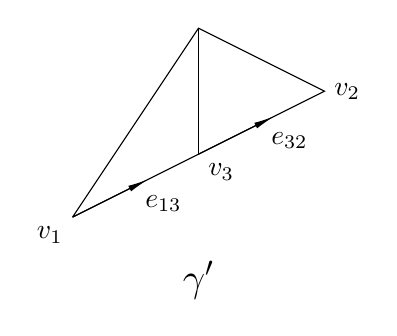
\begin{tikzpicture}[scale=0.8,]
					\node[below left] (v1) at (0,0) {$v_1$};
					\node[right] (v2) at (4,2) {$v_2$};
					\node[below right] (v3) at (2,1) {$v_3$};
					\node[below right] (e13) at (1,0.5) {$e_{13}$};
					\node[below right] (e32) at (3,1.5) {$e_{32}$};
					\draw[\myarrow] (0,0) -- (1.2,0.6);
					\draw[\myarrow] (2,1) -- (3.2,1.6);
					\draw (0,0) -- (4,2) -- (2,3) -- (0,0);
					\draw (2,1) -- (2,3);
					\node (gamma) at (2,-1) {{\Large $\gamma'$}};
				\end{tikzpicture}
				\caption{有偏序关系的图$\gamma$ 和 $\gamma'$}\label{figure-twogragh}
			\end{figure}

			为此,对于每一对图 $\gamma \prec \gamma'$ 引入图限制映射
			\begin{equation}
				p_{\gamma' \gamma} \colon \bar{\configurationspace{A}}_{\gamma'} \rightarrow \bar{\configurationspace{A}}_\gamma \qc h_{\gamma'} \mapsto \left.h_{\gamma'}\right|_{\gamma},
			\end{equation}
			它满足对于 $\gamma \prec \gamma' \prec \gamma''$ 有
			\begin{equation}
				p_{\gamma'' \gamma} = p_{\gamma' \gamma} \circ p_{\gamma'' \gamma'},
			\end{equation}
			则有
			\begin{equation}
				p_{\gamma' \gamma}\left( A_{\gamma'} \right) = A_\gamma,
			\end{equation}
			于是考虑如下定义
			\begin{Definition}
				投影系统(projective system)$\left\{ \bar{\configurationspace{A}}_\gamma, p_{\gamma' \gamma} \right\}$ 的\emph{投影极限}(projective limit)定义为 $\bar{\configurationspace{A}}_\infty$ 的一个子集
				\begin{equation}
					\varprojlim_{\gamma} \bar{\configurationspace{A}}_\gamma \definedby \left\{ {\left( h_\gamma \right)}_{\gamma \in \Gamma} \in \bar{\configurationspace{A}}_{\infty} \,\middle\vert\, p_{\gamma' \gamma}(h_{\gamma'}) = h_\gamma\qc \forall \gamma \prec \gamma' \right\}.
				\end{equation}
			\end{Definition}
			我们不加证明地列出以下结果:
			\begin{Property}
				\begin{enumerate}
					\item $p_{\gamma' \gamma}$ 都是连续满射;
					\item $\varprojlim_{\gamma} \bar{\configurationspace{A}}_\gamma$ 是 $\bar{\configurationspace{A}}_\infty$ 的闭子集,因而在子空间拓扑下也是紧致豪斯多夫空间;
					\item 映射
					\begin{equation}
						\Phi \colon \bar{\configurationspace{A}} \rightarrow \varprojlim_{\gamma} \bar{\configurationspace{A}}_\gamma \qc A \mapsto {\left( h_\gamma \definedby A|_\gamma \right)}_{\gamma \in \Gamma}
					\end{equation}
					是双射。
				\end{enumerate}
			\end{Property}
			至此,用 $\Phi$ 将 $\bar{\configurationspace{A}}$ 与 $\varprojlim_{\gamma} \bar{\configurationspace{A}}_\gamma$ 认同,即在 $\bar{\configurationspace{A}}$ 上定义了一个紧致豪斯多夫拓扑。

		\subsection{\texorpdfstring{$\bar{\configurationspace{A}}$上的测度}{量子位型空间上的测度}}

			上一节中为 $\bar{\configurationspace{A}}$ 定义的紧致豪斯多夫拓扑将对其上测度的定义起到很大帮助。本节定义 $\bar{\configurationspace{A}}$ 上的 Ashtekar-Lewandowski 测度,参见\cite{Ashtekar1994,Thiemann0210094,Thiemann2007}。

			考虑连续函数的集合 $C\left(\bar{\configurationspace{A}}\right)$,根据 Riesz-Markov-Kakutani 表示定理,由于 $\bar{\configurationspace{A}}$ 具有紧致豪斯多夫拓扑,其上的正则 Borel 测度 $\mu$ 与 $C\left(\bar{\configurationspace{A}}\right)$ 上的正定线性泛函 $\Lambda$ 通过下式一一对应
			\begin{equation}
				\Lambda\left(f\right) = \int_{\bar{\configurationspace{A}}} \dd{\mu} f \qc \forall f \in C\left(\bar{\configurationspace{A}}\right).
			\end{equation}
			注意到 $C\left(\bar{\configurationspace{A}}\right)$ 上可定义上确界范数 $\norm{f} \definedby \sup_{A \in \bar{\configurationspace{A}}} \abs{f(A)}$,可以检验 $C\left(\bar{\configurationspace{A}}\right)$ 构成 $C^*$-代数,则一个泛函分析中的标准结果是 $C\left(\bar{\configurationspace{A}}\right)$ 上的线性泛函自动是连续的,因而有界,且 $\norm{\Lambda} = \Lambda(1)$,故我们总可以选择 $\Lambda$ 使 $\Lambda(1)=1$,则 $\mu$ 是一个概率测度。

			为了明确定义一个 $\Lambda$,考察柱函数与 $C\left(\bar{\configurationspace{A}}\right)$ 的关系。这里重新定义一下 $\Cyl^k\left(\bar{\configurationspace{A}}\right)$ 以代替之前在 $\configurationspace{A}$ 上定义的 $\Cyl^k$。
			\begin{Definition}
				取两个 $k$ 阶可微的函数 $f_\gamma \in C^k\left(\bar{\configurationspace{A}}_\gamma\right)$ 与 $f_{\gamma'} \in C^k\left(\bar{\configurationspace{A}}_{\gamma'}\right)$\footnote{这里 $k$ 阶可微的定义是将 $\SU{2}^{\card{E(\gamma)}}$ 的光滑结构也搬到 $\bar{\configurationspace{A}}_\gamma$ 上定义的。},若它们满足任取 $\gamma''$ 使得 $\gamma , \gamma' \prec \gamma''$,有
				\begin{equation}
					p^*_{\gamma'' \gamma} f_\gamma = p^*_{\gamma'' \gamma'} f_{\gamma'},
				\end{equation}
				称 $f_\gamma$ 和 $f_{\gamma'}$ 是等价的,或 cylindrically consist,记为 $f_\gamma \sim f_{\gamma'}$。则定义 $\bar{\configurationspace{A}}$ 上的 $k$ 阶可微柱函数的集合为
				\begin{equation}
					\Cyl^k(\bar{\configurationspace{A}}) \definedby \left. \left( \bigcup_{\gamma \in \Gamma} C^k \left(\bar{\configurationspace{A}}_\gamma \right) \right) \middle/ \sim \right. ,
				\end{equation}
				特别地,有
				\begin{equation}
					\Cyl(\bar{\configurationspace{A}}) = \left. \left( \bigcup_{\gamma \in \Gamma} C\left(\bar{\configurationspace{A}}_\gamma\right) \right) \middle/ \sim \right. .
				\end{equation}
			\end{Definition}
			\begin{Remark}
				按照定义,每一个 $f_\gamma$ 可定义一个 $f= [f_\gamma] \in \Cyl^k\left(\bar{\configurationspace{A}}\right)$;每一个 $f\in \Cyl^k\left(\bar{\configurationspace{A}}\right)$ 都可找到合适的图 $\gamma$ 使 $f$ 有一个代表元 $f_\gamma$,即 $f=[f_\gamma]$;任取 $f,f' \in \Cyl^k\left(\bar{\configurationspace{A}}\right)$,可找到一个图 $\gamma$ 及 $f_\gamma, f^\prime_\gamma \in C^k\left(\bar{\configurationspace{A}}_\gamma\right)$ 使得 $f=[f_\gamma],f'=[f^\prime_\gamma]$。
			\end{Remark}

			容易验证,$C^k\left(\bar{\configurationspace{A}}_\gamma\right)$ 上通常的加法、乘法、数乘和复共轭可良定义到 $\Cyl^k\left(\bar{\configurationspace{A}}\right)$ 上,使其成为含幺阿贝尔 $*$-代数。在 $\Cyl\left(\bar{\configurationspace{A}}\right)$ 上也可定义上确界范数,并完备化得 $\overline{\Cyl\left(\bar{\configurationspace{A}}\right)}$,这是一个 $C^*$-代数,它正是 $C\left(\bar{\configurationspace{A}}\right)$\cite{Thiemann2007}。
			
			于是我们现在知道,$C\left(\bar{\configurationspace{A}}\right)$ 中的函数可视为 $\Cyl\left(\bar{\configurationspace{A}}\right)$ 中的柯西列 $\left\{ [f_\gamma] \right\}$。而 $\Lambda$ 连续,故只需关注 $\Lambda$ 在柱函数上的取值。这里为了绕开关于投影极限上测度的定理,不按照 Ashtekar 和 Lewandowski \cite{Ashtekar1994} 及 \cite{Thiemann2007} 的方式继续推导,而是直接引入 spin-network 的概念:
			\begin{Definition}
				\begin{enumerate}
					\item 给定一个图 $\gamma$,对每条边 $e\in E(\gamma)$ 标记一组数 $\left(j_e,m_e,n_e\right)$,其中 $j_e$ 是取半正整数的自旋量子数,$m_e$,$n_e$ 是在 $\left\{ -j_e, -j_e+1, \cdots , j_e \right\}$ 中取值的磁量子数,则四元组
					\begin{equation}
						s \definedby \left( \gamma, \myvec{j} \definedby (j_e)_{e\in E(\gamma)}, \myvec{m} \definedby (m_e)_{e\in E(\gamma)}, \myvec{n} \definedby (n_e)_{e\in E(\gamma)} \right)
					\end{equation}
					称为一个\emph{自旋网络}(spin-network,简写为 SNW)。
					\item 记 Wigner D-矩阵
					\begin{equation}
						\tensor{D}{^j_m_n}(g) = \mel{jm}{\rho^j(g)}{jn},
					\end{equation}
					其中 $\rho_j$ 是 $\SU{2}$ 的 spin-$j$ 不可约表示,则称
					\begin{equation}
						T_s \colon \bar{\configurationspace{A}} \rightarrow \mathbb{C} \qc A \mapsto \prod_{e\in E(\gamma)} \sqrt{2j_e + 1} \tensor{D}{^{j_e}_{m_e}_{n_e}}(A(e))
					\end{equation}
					为 $s$ 的 spin-network function(SNWF),并额外定义 $T_{(\emptyset, \myvec{0},\myvec{0},\myvec{0})} = 1$。
				\end{enumerate}
			\end{Definition}
			使用 SNWF 的动机之一是它们是互相线性独立的,而不像 Wilson loop 有 Mandelstam 恒等式互相联系。%由 Peter-Weyl 定理,$\tensor{\pi}{^j_m_n} = \sqrt{2j+1} \tensor{D}{^j_m_n}$ 构成 $L^2(\SU{2},\mu_H)$ 的一组正交归一基底,其中 $\mu_H$ 是哈尔测度(Haar measure),则某个图上面的所有 SNWF 构成 $L^2(\bar{\configurationspace{A}}_\gamma, \mu_H^{\card{E(\gamma)}})$ 的正交归一基,$\Span \left\{ T_{s} \right\}_{s=(\gamma,\cdot,\cdot,\cdot)}$ 在 $C(\bar{\configurationspace{A}}_\gamma)$ 中稠密。
			根据 Stone-Weierstrass 定理,$\Span\left\{ T_s \right\}$ 在 $C(\bar{\configurationspace{A}})$ 中稠密,所以只需关心 $\Lambda$ 在 SNWF 上的取值。以下定义 Ashtekar-Lewandowski 测度:
			\begin{Definition}
				Ashtekar-Lewandowski 测度 $\mu_{\text{A-L}}$ 由以下正定线性泛函唯一确定:
				\begin{equation}
					\Lambda_{\text{A-L}}(T_s) \definedby
					\begin{cases}
						1, & s=\left(\emptyset,\myvec{0},\myvec{0},\myvec{0}\right),\\
						0, & \text{otherwise}.
					\end{cases}
				\end{equation}
			\end{Definition}
			于是可定义 $\Hkin \definedby L^2\left(\bar{\configurationspace{A}},\mu_{\text{A-L}}\right)$。

			\nomenclature{$T_s$}{spin-network function}
			\nomenclature{$\mu_{\text{A-L}}$}{Ashtekar-Lewandowski 测度}

			可以通过群表示的计算证明:
			\begin{Property}
				\begin{enumerate}
					\item SNWF 构成 $\Hkin$ 的一组正交归一基底。
					\item 任取 $f=[f_\gamma] \in \Cyl\left(\bar{\configurationspace{A}}\right)$,有
					\begin{equation}
						\int_{\bar{\configurationspace{A}}} \dd{\mu_{\text{A-L}}} f = \Lambda_{\text{A-L}}(f) = \int_{\SU{2}^{\card{E(\gamma)}}} \left( \prod_{e\in E(\gamma)} \dd{\mu_H}(h_e) \right) f_\gamma\left( h_{e_1}, \cdots, h_{e_{\card{E(\gamma)}}} \right),
					\end{equation}
					特别地,任取 $f=[f_\gamma]$,$f'=[f^\prime_\gamma]$,
					\begin{equation}
						\begin{split}
							&\ip{f}{f'}_{\text{kin}} \definedby \int_{\bar{\configurationspace{A}}} \dd{\mu_{\text{A-L}}} \bar{f} f'\\
							={}& \int_{\SU{2}^{\card{E(\gamma)}}} \left( \prod_{e\in E(\gamma)} \dd{\mu_H}(h_e) \right) \overline{f_\gamma\left( h_{e_1}, \cdots, h_{e_{\card{E(\gamma)}}} \right)}f^\prime_\gamma\left(h_{e_1}, \cdots, h_{e_{\card{E(\gamma)}}}\right).
						\end{split}
					\end{equation}
				\end{enumerate}
			\end{Property}
			由于 $\bar{\configurationspace{A}}_\gamma$ 与 $\SU{2}^{\card{E(\gamma)}}$ 认同,不妨记 $\mu_\gamma$ 为测度
			\begin{equation}
				\int_{\bar{\configurationspace{A}}_\gamma} \dd{\mu_\gamma} f_\gamma = \Lambda_\gamma(f_\gamma) \definedby \int_{\SU{2}^{\card{E(\gamma)}}} \left( \prod_{e\in E(\gamma)} \dd{\mu_H}(h_e) \right) f_\gamma\left(h_{e_1}, \cdots, h_{e_{\card{E(\gamma)}}}\right),
			\end{equation}
			并定义
			\begin{equation}
				\Hil_\gamma \definedby L^2\left(\bar{\configurationspace{A}}_\gamma,\mu_\gamma\right) = L^2 \left(\SU{2}^{\card{E(\gamma)}}, \mu_H^{\card{E(\gamma)}} \right) = \otimes^{\card{E(\gamma)}} L^2\left(\SU{2}, \mu_H\right),
			\end{equation}
			将 $e\in E(\gamma)$ 也看作图,又有 $\Hil_e = L^2\left(\bar{\configurationspace{A}}_e,\mu_e\right) = L^2\left(\SU{2}, \mu_H\right)$,则又有 $\Hil_\gamma = \bigotimes_{e\in E(\gamma)} \Hil_e$。还有一个有用的结果是
			\begin{Property}
				\begin{equation}
					\Hkin = \left\langle \Cyl\left( \bar{\configurationspace{A}} \right) \right\rangle = \left\langle \bigcup_{\gamma \in \Gamma} \Hil_\gamma \right\rangle,
				\end{equation}
				其中 $\left\langle \cdot \right\rangle$ 表示对于 $\ip{\cdot}_{\text{kin}}$ 取完备化。
			\end{Property}
			因此,我们常常能把 $\Hkin$ 上的问题转变为 $\Hil_\gamma$ 上的问题,而后者直观得多。

			\nomenclature{$\Hkin$}{kinematical 希尔伯特空间}
			\nomenclature{$\Hil_\gamma$}{图 $\gamma$ 上的kinematical 希尔伯特空间}

		\subsection{\texorpdfstring{$\staralgebra{B}$ 在 $\Hkin$ 上的表示}{B 在希尔伯特空间 H 上的表示}}

			本节定义 $\staralgebra{B}$ 在 $\Hkin$ 上唯一的不可约表示。此表示的严格定义及唯一性的证明参见 \cite{Thiemann2007}。

			按照定义 $\Cyl^k(\bar{\configurationspace{A}})$ 的方式,可在 $\left\{ V^k\left(\bar{\configurationspace{A}}_\gamma\right) \cong V^k\left(\SU{2}^{\card{E(\gamma)}}\right) \right\}_{\gamma\in \Gamma}$ 上定义等价关系 $\sim$,并定义
			\begin{equation}
				V^k\left( \bar{\configurationspace{A}} \right) \definedby \left. \left( \bigcup_{\gamma\in \Gamma} V^k\left( \bar{\configurationspace{A}}_\gamma \right) \right) \middle/ \sim \right. ,
			\end{equation}
			这里只需知道 $v^i_S \in V^\infty\left( \bar{\configurationspace{A}} \right)$。选择 $\Dkin \definedby \Cyl^\infty \left( \bar{\configurationspace{A}} \right)$,定义由下式确定的表示
			\begin{equation}
				\begin{split}
					\left( \pi(f)f' \right)(A) &\definedby (f f')(A),\\
					\left( \pi\left(v^i_S\right) f \right)(A) &\definedby \ii\hbar \left( v^i_S(f) \right)(A),\\
					\pi(a) &\definedby \pi(f) + \pi\left(v^i_S\right),
				\end{split}
			\end{equation}
			其中 $f,f'\in \Cyl^\infty\left(\bar{\configurationspace{A}}\right)$,$v^i_S = \left\{ P_i(S), \cdot \right\} \in V^\infty \left( \bar{\configurationspace{A}} \right)$,$a=\left( f, v^i_S \right) \in \staralgebra{B}$。则容易验证
			\begin{equation}
				\left[ \pi(a), \pi(b) \right] = \pi\left( \left[ a,b \right] \right).
			\end{equation}
			对于 $*$-运算,首先容易验证 $\pi(f)^\dagger = \pi(\bar{f})$;$\bar{v}^i_S = v^i_S$,而由~\eqref{eq-flux_function_algebra} 知
			\begin{equation}
				\pi\left(v^i_S\right) = \frac{\hbar}{2} \sum_{v\in V(\gamma) \cap S} \left( \sum_{e:v\in e} \kappa(S,e) \hat{J}^{(e,v)}_i \right),\label{eq-flux_operator}
			\end{equation}
			其中 $v\in e$ 表示 $v$ 是 $e$ 的端点,而 $\hat{J}^{(e,v)}_i$ 的定义如下,先定义 $\Hil_e = L^2(\SU{2},\mu_H)$ 上的两个角动量算符
			\begin{equation}
				\hat{J}^{(L)}_i \definedby \ii L_i \qc \hat{J}^{(R)}_i \definedby \ii R_i,
			\end{equation}
			其中 $L_i$ 和 $R_i$ 是左不变和右不变矢量场。容易检查它们自伴。对于 $\Hil_\gamma = \bigotimes_{e\in E(\gamma)} \Hil_e$,任取 $v\in V(\gamma)$,$e\in E(\gamma)$,定义
			\begin{equation}
				\hat{J}^{(e,v)}_i \definedby
				\begin{cases}
					\ii L^{(e)}_i, & v=s(e),\\
					\ii R^{(e)}_i, & v=t(e),\\
					0, & \text{else},
				\end{cases}
			\end{equation}
			其中 $L_i^{(e)}$ 和 $R_i^{(e)}$ 是~\eqref{eq-invariance_vector_field} 中定义的左不变和右不变矢量场。$\hat{J}^{(e,v)}_i$ 可以被写为
			\begin{equation}
				\hat{J}^{(e,v)}_i =
				\begin{cases}
					\hat{\II} \otimes \cdots \otimes \hat{J}_i^{(L)} \otimes \cdots \otimes \hat{\II}, & v=s(e),\\
					\hat{\II} \otimes \cdots \otimes \hat{J}_i^{(R)} \otimes \cdots \otimes \hat{\II}, & v=t(e),\\
					0, & \text{else},
				\end{cases}
			\end{equation}
			则它显然是自伴的。于是由~\eqref{eq-flux_operator} 知 $\pi\left(v^i_S\right)$ 自伴。故 $\pi$ 保泊松括号、$*$-运算,它的确是一个表示。
			\begin{Theorem}
				表示 $\pi$ 是 $\staralgebra{B}$(的泛包络代数$\staralgebra{A}$)的不可约表示,且在一定的限制条件下有唯一性。
			\end{Theorem}
			\begin{Proof}
				这里证明 $\pi$ 的不可约。由于 $\bar{\configurationspace{A}}$ 紧致,$f$ 必有界,故 $\pi(f)$ 是有界算子,它实际上定义在整个 $\Hkin = L^2(\bar{\configurationspace{A}},\mu_{\text{A-L}})$。令 $\Omega = 1 \in \Cyl^\infty(\bar{\configurationspace{A}})$,则 $\pi(f) \Omega = f$ 即跑遍 $\Hkin$ 的一个稠密子空间 $\Dkin = \Cyl^\infty(\bar{\configurationspace{A}})$,故 $\Omega$ 是 cyclic vector。故 $\pi$ 不可约。
			\end{Proof}
	
	% !TeX root = ../NotesOnLQG.tex

\chapter{量子约束的求解及动力学}

	本章将在量子理论中求解约束~\eqref{eq-constrains_in_Ashtekar_connection}:
	\begin{equation*}
		\begin{split}
			\tensor{G}{_i} &= \AD{a} \tensor{\tilde{P}}{^a_i} = \Partial{a} \tensor{\tilde{P}}{^a_i} + \tensor{\vol}{_i_j^k} \tensor{A}{^j_a} \tensor{\tilde{P}}{^a_k},\\
			\tensor{V}{_a} &= \tensor{\tilde{P}}{^b_i} \tensor{F}{^i_a_b} - \frac{1+\gamma^2}{\gamma} \tensor{K}{^i_a} \tensor{G}{_i},\\
			C &= \frac{\gkappa \gamma^2}{2\sqrt{\abs{\det h}}} \tensor{\tilde{P}}{^a_i} \tensor{\tilde{P}}{^b_j} \left[ \tensor{\vol}{^i^j_k} \tensor{F}{^k_a_b} - \left( 1+ \gamma^2 \right) \tensor{K}{^i_a} \wedge \tensor{K}{^j_b} \right]\\
			& \qquad + \gkappa \left( 1 +\gamma^2 \right) \tensor{G}{^i} \Partial{a} \left( \frac{\tensor{\tilde{P}}{^a_i}}{\sqrt{\abs{\det h}}} \right).
		\end{split}
	\end{equation*}
	回忆它们的约束代数~\eqref{eq-constrain_algebra},我们曾经提起过高斯约束构成双边理想,可以先独立解出,而且能直接在 $\Hkin$ 上求解得到 $\SU{2}$ 不变空间 $\Hkin^0$,较为简单。之后将以 $\Hkin^0$ 为 kinematical 希尔伯特空间,继续求解其他约束。

	\section{量子高斯约束}

		在~\eqref{eq-smeared_Gauss_constrain} 中定义了经典的 smeared 高斯约束
		\begin{equation}
			G(\Lambda) = \int_{\spc} \dd[3]{x} \tensor{\Lambda}{^i} \AD{a} \tensor{\tilde{P}}{^a_i} = - \int_{\spc} \dd[3]{x} \tensor{\tilde{P}}{^a_i} \AD{a} \tensor{\Lambda}{^i},
		\end{equation}
		这是动量在3维的smear,将 $\int_{\spc} \dd[3]{x} \tensor{\tilde{P}}{^a_i} \AD{a} \tensor{\Lambda}{^i}$ 记为 $P(\ADd \Lambda)$,并定义 $\bar{\configurationspace{A}}$ 上的矢量场
		\begin{equation}
			Y_{\ADd \Lambda}([f_\gamma]) \definedby \left\{ - P(\ADd \Lambda), f_\gamma \right\},
		\end{equation}
		则高斯约束可自然被量子化为
		\begin{equation}
			\begin{split}
				\hat{G}(\Lambda) f &\definedby \ii\hbar Y_{\ADd \Lambda}(f)\\
				&= \hbar \sum_{v\in V(\gamma)} \tensor{\Lambda}{^i}(v) \hat{J}^v_i f_\gamma,
			\end{split}
		\end{equation}
		其中
		\begin{equation}
			\hat{J}^v_i \definedby \sum_{e:v\in e} \hat{J}^{(e,v)}_i,
		\end{equation}
		于是根据群表示的知识,$\hat{G}(\Lambda)$ 具有点谱,是可以直接在 $\Hkin$ 上求解的,量子高斯约束方程是
		\begin{equation}
			\hat{J}^v_i f_\gamma =0\qc \forall v \in V(\gamma),
		\end{equation}
		或等价地
		\begin{equation}
			\left( \hat{J}^v \right)^2 f_\gamma =0\qc \forall v \in V(\gamma),
		\end{equation}
		其中 $\left( \hat{J}^v \right)^2 \definedby \tensor{\delta}{^i^j} \hat{J}^v_i \hat{J}^v_j$。

		为了求解量子高斯约束方程,我们重新观察之前构造的 $\Hkin$ 的一组基底——spin-network function。注意到 $\Hil_\gamma = \bigotimes_{e\in E(\gamma)} \Hil_e$,而 $\Hil_e \cong L^2(\SU{2},\mu_H)$ 上 $\left\{ \hat{J}^2, \hat{J}^{(L)}_3, \hat{J}^{(R)}_3 \right\}$ 构成完备对易算符集,其中
		\begin{equation}
			\hat{J}^2 \definedby \tensor{\delta}{^i^j} \hat{J}^{(L)}_i \hat{J}^{(L)}_j \equiv \tensor{\delta}{^i^j} \hat{J}^{(R)}_i \hat{J}^{(R)}_j
		\end{equation}
		它们的共同本征态就是 $\tensor{\pi}{^j_m_n}$:
		\begin{equation}
			\hat{J}^2 \tensor{\pi}{^j_m_n} = j(j+1) \tensor{\pi}{^j_m_n} \qc \hat{J}^{(L)}_3 \tensor{\pi}{^j_m_n} = m \tensor{\pi}{^j_m_n} \qc \hat{J}^{(R)}_3 \tensor{\pi}{^j_m_n} = n \tensor{\pi}{^j_m_n},
		\end{equation}
		故以 $\tensor{\pi}{^j_m_n}$ 为基底就是在算符集 $\left\{ \hat{J}^2, \hat{J}^{(L)}_3, \hat{J}^{(R)}_3 \right\}$ 下分解 $\Hil_e$。这可以通过 $\tensor{\pi}{^j_m_n}(g) = \mel{jm}{\rho^j(g)}{jn} = \tr(\op{jn}{jm}\rho^j(g))$ 从另一方面理解,映射
		\begin{equation}
			\op{jn}{jm} \mapsto \tensor{\pi}{^j_m_n} = \tr(\op{jn}{jm}\rho^j(\cdot))
		\end{equation}
		是 $\bigoplus_j \left( \Hil_j \otimes \Hil_j^* \right)$ 到 $\Hil_e$ 的同构,其中 $\Hil_j$ 是 $\SU{2}$ 的 spin-$j$ 表示空间。$\hat{J}^{(L)}_i$ 可理解为作用在左矢 $\bra{jm}$,即是 $\Hil_j^*$ 上的角动量算符,而 $\hat{J}^{(R)}_i$ 可理解为作用在右矢 $\ket{jn}$,即是 $\Hil_j$ 上的角动量算符。
		于是 spin-network function 作为 $\tensor{\pi}{^j_m_n}$ 的张量积,是完备对易算符集 $\left\{ \left( \hat{J}^{(e)} \right)^2, \hat{J}^{(e,s(e))}_3, \hat{J}^{(e,t(e))}_3 \right\}_{e\in E(\gamma)}$ 的共同本征函数,对应于分解
		\begin{equation}
			\begin{split}
				\Hil_\gamma &= \bigotimes_{e\in E(\gamma)} \Hil_e = \bigotimes_{e\in E(\gamma)} \left( \bigoplus_{j_e} \left( \Hil^{(e)}_{j_e} \otimes \Hil^{(e)*}_{j_e} \right) \right)\\
				&= \bigoplus_{\myvec{j}} \left( \bigotimes_{e\in E(\gamma)} \left( \Hil^{(e)}_{j_e} \otimes \Hil^{(e)*}_{j_e} \right) \right),\label{eq-spin_network_function_decompose}
			\end{split}
		\end{equation}
		量子高斯约束算符中的 $\hat{J}^v_i = \sum_{e:v\in e} \hat{J}^{(e,v)}_i$ 提示我们在顶点处进行角动量耦合。定义
		\begin{equation}
			\Hil_j^{(e,v)} \definedby
			\begin{cases}
				\Hil_j, & v=t(e),\\
				\Hil_j^*, & v=s(e),\\
				\left\{ 0 \right\}, & \text{otherwise},
			\end{cases}
		\end{equation}
		则可继续改写
		\begin{equation}
			\begin{split}
				\Hil_\gamma &= \bigoplus_{\myvec{j}} \left( \bigotimes_{e\in E(\gamma)} \left( \bigotimes_{\substack{v:v\in e}} \Hil_{j_e}^{(e,v)} \right) \right) = \bigoplus_{\myvec{j}} \left( \bigotimes_{v\in V} \left( \bigotimes_{\substack{e:v\in e}} \Hil_{j_e}^{(e,v)} \right) \right),
			\end{split}
		\end{equation}
		顶点 $v$ 处的张量积表示 $\bigotimes_{\substack{e:v\in e}} \Hil_{j_e}^{(e,v)}$ 就是 $\hat{J}_i^{v}$ 作用的空间,可分解为不可约表示的直和
		\begin{equation}
			\bigotimes_{\substack{e:v\in e}} \Hil_{j_e}^{(e,v)} = \bigoplus_{l} \Hil_{\myvec{j}(v),l_v}^{v},
		\end{equation}
		其中 $l_v$ 是 $\left( \hat{J}^{v} \right)^2$ 的量子数,$\myvec{j}(v) = \left( j_e \right)_{v\in e}$ 是所有以 $v$ 为端点的边上标记的 $j_e$ 的数组。故
		\begin{equation}
			\Hil_\gamma = \bigoplus_{\myvec{j}} \left( \bigoplus_{\myvec{l}} \left( \bigotimes_{v\in V(\gamma)} \Hil_{\myvec{j}(v),l_v}^{v} \right) \right),
		\end{equation}
		则 $\Hil_\gamma$ 中量子高斯约束的解空间即为
		\begin{equation}
			\Hil_\gamma^0 \definedby \bigoplus_{\myvec{j}} \left( \bigotimes_{v\in V(\gamma)} \Hil_{\myvec{j}(v),l_v=0}^{v} \right),\label{eq-H0gamma_decompose}
		\end{equation}
		注意到
		\begin{equation}
			\Hil_{\myvec{j}(v),l_v=0}^{v} = \Inv\left( \bigotimes_{\substack{e:v\in e}} \Hil_{j_e}^{(e,v)} \right)
		\end{equation}
		是数学中所说的 intertwiner space,可依照分解式~\eqref{eq-H0gamma_decompose} 给出 $\Hil_\gamma^0$ 的一组基底:
		\begin{Definition}
			任给定图 $\gamma$,指定 $\myvec{j} = \left( j_e \right)_{e\in E(\gamma)}$,使得每个顶点处 $\bigotimes_{\substack{e:v\in e}} \Hil_{j_e}^{(e,v)}$ 都存在 intertwiner;然后对每个顶点指定一个 intertwiner $i_v \in \Hil_{\myvec{j}(v),l_v=0}^{v}$,记规范不变的spin-network 为 $s=(\gamma,\myvec{j},\myvec{i})$,则定义\emph{spin-network state}为
			\begin{equation}
				\psi_s(A) \definedby \operatorname{C} \left( \bigotimes_{v\in V(\gamma)} i_v \bigotimes_{e\in E(\gamma)} \rho^j(A(e)) \right),
			\end{equation}
			其中 $\operatorname{C}(\cdot)$ 指对每一对 $(e,v)$ 将 intertwiner $i_v$ 与 $\rho^j(A(e))$ 相对应的指标缩并。

			当 $\myvec{j}$ 取遍且 $i_v$ 取遍 intertwiner space 取定的一组基底时,spin-network state 构成 $\Hil_\gamma^0$ 的基底。
		\end{Definition}
		对于整个 $\Hkin$,则需要一些新定义和一个分解定理\cite{Han2005}:
		\begin{Definition}
			对图 $\gamma$,若 $v\in V(\gamma)$ 满足:以 $v$ 为顶点的边有且只有两条,且都不是以 $v$ 为基点的圈(loop),即都只过 $v$ 一次,并且它们相乘($\circ$运算)是解析的,则称 $v$ 为\emph{伪顶点}。换句话说,伪顶点人为地将一条边分为两条。
			
			定义
			\begin{equation}
				\Hil_\gamma^\prime = \bigoplus_{\left( \myvec{j},\myvec{l} \right) \in I_\gamma} \left( \bigotimes_{v\in V(\gamma)} \Hil_{\myvec{j}(v),l_v}^{v} \right),
			\end{equation}
			其中 $I_\gamma$ 对 $\myvec{j}$ 和 $\myvec{l}$ 作如下两条限定:所有 $j_e \neq 0$;对每个伪顶点,$l\neq 0$。
		\end{Definition}
		\begin{Theorem}
			$\Hkin$ 有直和分解
			\begin{equation}
				\Hkin = \left( \bigoplus_{\gamma \in \Gamma} \Hil_\gamma^\prime \right) \oplus \mathbb{C}.
			\end{equation}
		\end{Theorem}
		每个 $\Hil_\gamma^\prime$ 不过是对 $\left( \myvec{j}, \myvec{l} \right)$ 作限制,对量子高斯约束方程没有影响,故在 $\Hil_\gamma^\prime$ 中的规范不变子空间为
		\begin{equation}
			\Hil_\gamma^{0\prime} = \bigoplus_{\left( \myvec{j},\myvec{l}=\myvec{0} \right) \in I} \left( \bigotimes_{v\in V(\gamma)} \Hil_{\myvec{j}(v),l_v=0}^{v} \right),
		\end{equation}
		$\Hil_\gamma^{0\prime}$ 的基底也只需对 spin-network state 的 $\myvec{j}$ 作出限制即可。于是可直接得到
		\begin{Theorem}
			高斯约束的解子空间为
			\begin{equation}
				\Hkin^0 = \left( \bigoplus_{\gamma \in \Gamma} \Hil_\gamma^{0\prime} \right) \oplus \mathbb{C},
			\end{equation}
			其上的一组基底是
			\begin{equation}
				\left\{ \psi_{s=(\gamma,\myvec{j},\myvec{i})} \,\middle|\, (\myvec{j},\myvec{0}) \in I_\gamma, \text{每个 $i_v$ 在取定的一组基底中取值}, \gamma\in \Gamma \right\}.
			\end{equation}
		\end{Theorem}
		定义 $\Cyl\left(\overline{\configurationspace{A}/\configurationspace{G}}\right) = \Span\{\psi_{s}\}$,它在 $\Hkin^0$ 中稠密,将用作求解其他约束的 $\Dkin^0$,并记 $\Cyl_\gamma\left(\overline{\configurationspace{A}/\configurationspace{G}}\right) = \Span\left\{\psi_{s}\,\middle|\,\gamma(s) = \gamma\right\}$ 。

		\nomenclature{$\Hkin^0$}{$\Hkin$中规范不变的态空间}

	\section{量子微分同胚约束}

		与高斯约束不同的是,微分同胚约束 $C_{\text{Diff}}(v)$ 本身没有良好的算符定义,即找不到 $\Dkin$ 算符 $\hat{C}_{\text{Diff}}(v)$。空间微分同胚群在 $\Dkin^0$ 上有自然的酉表示
		\begin{equation}
			\hat{U}_{\varphi} f_\gamma \definedby f_{\varphi \circ \gamma},
		\end{equation}
		它保持 $\mu_{\text{A-L}}$ 不变,且无反常,即
		\begin{equation}
			\hat{U}_{\varphi} \hat{U}_{\varphi'} \hat{U}_{\varphi}^{-1} \hat{U}_{\varphi^{\prime}}^{-1} = \hat{U}_{\varphi \circ \varphi' \circ \varphi^{-1} \circ {\varphi'}^{-1}},
		\end{equation}
		但该表示不是弱连续的,故无法定义其生成元算符。因此,要求解的不是 $\hat{C}_{\text{Diff}} = 0$,而是 $\hat{U}_{\varphi} = \II$。

		按照第\ref{chp-Quantization}章第\ref{sec-Quantization}节中介绍的 RAQ,需要求解 $l\in (\Dkin^0)^*$,使得
		\begin{equation}
			l\left(\hat{U}_\varphi f\right) = l(f) \qc \forall \varphi \in \Diff{\spc}, f\in \Dkin^0,\label{eq-Quantum_Diff_equation}
		\end{equation}
		将 $l$ 展开为
		\begin{equation}
			l(f) = \sum_{s} c_s \ip{\psi_s}{f}_{\text{kin}},
		\end{equation}
		其中 $s=(\gamma,\myvec{j},\myvec{i})$ 取遍规范不变的spin-network,则~\eqref{eq-Quantum_Diff_equation} 等价于
		\begin{equation}
			\hat{U}^*_{\varphi}l = \sum_s c_s \bra{\psi_{\varphi \cdot s}} = \sum_{s'} c_{\varphi^{-1} \cdot s'} \bra{\psi_{s'}} = l,
		\end{equation}
		这要求
		\begin{equation}
			c_{s=(\gamma,\myvec{j},\myvec{i})} = c_{\varphi \cdot s = \varphi(\gamma),\myvec{j},\myvec{i}}\qc \forall \varphi \in \Diff{\spc},
		\end{equation}
		故 $c_s = c_{\gamma,\myvec{j},\myvec{i}}$ 对 $\gamma$ 的依赖实际上是依赖于 $\gamma$ 所在的微分同胚不变等价类 $[\gamma]$,这与扭结不变量是类似的。记 $\mathcal{N}$ 为 spin-network 的微分同胚等价类 $[s]$ 的集合,其中的元素记为 $\nu$,定义
		\begin{equation}
			l_{\nu}(\cdot) \definedby \sum_{s\in \nu} \ip{\psi_s}{\cdot}_{\text{kin}},
		\end{equation}
		则任意~\eqref{eq-Quantum_Diff_equation} 的解具有形式
		\begin{equation}
			l = \sum_{\nu \in \mathcal{N}} c_\nu l_\nu,
		\end{equation}
		这样就得到了 $\DDiff^*$。关于进一步定义 $\ip{\cdot}_{\text{Diff}}$ 及 $\HDiff$ 可参见 \cite{Han2005,Thiemann2007} 等。

		\nomenclature{$\DDiff^*$}{微分同胚约束的解空间}

	\section{量子动力学——哈密顿约束}

		这里我们遇到了正则圈量子引力的困难问题之一。在第\ref{chp-Quantization}章第\ref{sec-pre}节中提到过微分同胚约束与哈密顿约束泊松括号不为零的问题,这里表现为 哈密顿约束算符不能在 $\HDiff$ 上良好定义。Thiemann 通过对经典哈密顿约束进行一定的正规化,在 $\Hkin$ 上定义了哈密顿约束算符\cite{Thiemann1996aw},但它不与 $\hat{U}_{\varphi}$ 对易,使得无法将其定义在 $\HDiff$ 上。另外,哈密顿约束与自己的泊松括号存在结构函数
		\begin{equation}
			\left\{ C_{\text{H}}(f), C_{\text{H}}(f') \right\} = - C_{\text{Diff}}(S(f,f'))
		\end{equation}
		还导致了量子反常,这是应当避免的。

		从以上简要介绍可以看到,困难主要是由约束代数引起的。若可重新改写约束代数,使其构成李代数,并使微分同胚约束构成理想,则困难将得到很大程度地解决。这样的约束代数由 Thiemann 首次引入\cite{Thiemann2003zv},核心想法是引入主约束
		\begin{equation}
			\masterconstraint{M} \definedby \frac{1}{2} \int_{\spc} \dd[3]{x} \frac{\abs{\tilde{C}(x)}^2}{\sqrt{\abs{\det{h}}}}
		\end{equation}
		来代替
		\begin{equation}
			C_{\text{H}}(f) = \int_{\spc} \dd[3]{x} f(x) \tilde{C}(x),
		\end{equation}
		在经典层面,$\masterconstraint{M} = 0$ 等价于 $C_{\text{H}}(f) = 0, \forall f$,但极大地简化了约束代数
		\begin{equation}
			\begin{split}
				\left\{ C_{\mathrm{Diff}}(u), C_{\text{Diff}}(v) \right\} &= C_{\text{Diff}}([u,v]),\\
				\left\{ C_{\text{Diff}}(v), \masterconstraint{M} \right\} &= 0,\\
				\left\{ \masterconstraint{M}, \masterconstraint{M} \right\} &= 0,\label{eq-master_constrain_algebra}
			\end{split}
		\end{equation}
		这种方法已经在很多约束系统中经过了检验\cite{Dittrich:2004bn,Dittrich:2004bp,Dittrich:2004bq,Dittrich:2004br,Dittrich:2004bs}。为定义主约束算符,对主约束进行正规化
		\begin{equation}
			\masterconstraint{M}^\epsilon \definedby \frac{1}{2} \int_{\spc} \dd[3]{x} \int_{\spc} \dd[3]{y} \chi_\epsilon(x,y) \frac{\tilde{C}(x) \tilde{C}(y)}{\sqrt{\abs{\det{h}}}},
		\end{equation}
		其中 $\chi_\epsilon(x,y)$ 满足 $\lim_{\epsilon \rightarrow 0} \chi_\epsilon(x,y) = \delta(x,y)$,并引入三角剖分来逼近难以写成算符的 $\det{h}$。量子化后,最终令 $\epsilon \rightarrow 0$ 来得到主约束算符 $\hat{\masterconstraint{M}}$。主约束算符的细节超出了本文的范围,这里只介绍一些它的性质:$\hat{\masterconstraint{M}}$ 是在 $\HDiff$ 上稠定的,并且是可闭算符,其闭包 $\hat{\bar{\masterconstraint{M}}}$ 是 $\hat{\masterconstraint{M}}$ 唯一的自伴扩张,称为 Friedrichs 扩张。约束代数~\eqref{eq-master_constrain_algebra} 没有量子反常,即
		\begin{equation}
			\left[ \hat{\masterconstraint{M}}, \hat{U}_{\varphi} \right] = 0 \qc \left[ \hat{\masterconstraint{M}}, \hat{\masterconstraint{M}} \right] = 0.
		\end{equation}
		另外,0确实是属于 $\hat{\masterconstraint{M}}$ 的谱的,不需要平移算符 $\hat{\masterconstraint{M}}$\cite{Thiemann:2005zg}。在\cite{Giesel:2006uj,Giesel:2006uk}中,Giesel 和 Thiemann 证明了主约束算符具有正确的经典极限。

		\nomenclature{$\masterconstraint{M}$}{主约束}

		按照第\ref{chp-Quantization}章第\ref{sec-Quantization}节中的量子化程序,还需进一步研究的问题有:
		\begin{enumerate}
			\item 求解
			\begin{equation}
				\Hkin \cong \int_{\sigma(\masterconstraint{M})}^{\oplus} \dd{\mu}(\lambda) \Hkin^\oplus(\lambda)
			\end{equation}
			中的 $\Hkin^\oplus(0)$。由于主约束算符本身的复杂性,该问题尚未完全解决;
			\item 找出狄拉克观测量。在引力理论中寻找狄拉克观测量一直是个难题,但主约束算符提供了一条道路。若记 $\hat{U}(t)$ 是 $\hat{\masterconstraint{M}}$ 生成的单参酉算子群,若 $\hat{O}$ 是 $\HDiff$ 上的算符,且
			\begin{equation}
				\hat{[O]}\definedby \lim_{T\rightarrow \infty} \int_{-T}^T \dd{t} \hat{U}^{-1}(t) \hat{O} \hat{U}(t)\label{eq-group_average}
			\end{equation}
			收敛,则 $\hat{[O]}$ 与 $\hat{\masterconstraint{M}}$ 对易,是强狄拉克观测量。利用~\eqref{eq-group_average} 寻找狄拉克观测量是尚未解决的问题。
		\end{enumerate}

	% !TeX root = ../NotesOnLQG.tex

\chapter{正则圈量子引力的应用及发展}
\label{chp-application}

	正则圈量子引力已定义了希尔伯特空间,关于其上的物理一直处于探索中。这里只简单介绍几何量算符和相干态,并叙述圈量子宇宙学的状况。

	\section{量子几何——面积算符}

		经典理论中,空间几何是黎曼几何,本节将展示在圈量子引力中,长度、面积、体积等几何量将具有分立的谱。在圈量子引力中已定义的几何量有面积算符\cite{Rovelli1994,Ashtekar:1996eg}、体积算符\cite{Ashtekar:1994wa,Rovelli1994,Ashtekar:1997fb}和长度算符\cite{Thiemann:1996at}等,这里简要介绍较为简单的面积算符。

		设 $S$ 是 $\spc$ 中的一张解析、紧致且可定向的2维曲面,且有嵌入映射 $i_S \colon S \rightarrow \spc$,$S$ 上的坐标记为 $(u^1,u^2)$。则 $S$ 的面积是
		\begin{equation}
			A_S = \int_S \dd[2]{u} \sqrt{\det(i^*_S h)},
		\end{equation}
		借助坐标 $(u^1,u^2)$ 可算得
		\begin{equation}
			\det(i^*_S h) = \tensor{\tilde{E}}{^a_i} \tensor{n}{_a} \tensor{\tilde{E}}{^b_j} \tensor{n}{_b} \tensor{\delta}{^i^j},
		\end{equation}
		其中
		\begin{equation}
			\tensor{n}{_a} \definedby \tensor{\nvol}{_a_b_c} \tensor{\left( \pdv{u^1} \right)}{^b} \tensor{\left( \pdv{u^2} \right)}{^c}
		\end{equation}
		是 $S$ 上的法矢。
		注意到在 $S$ 很小时,
		\begin{equation}
			P_i(S) = \int_S \tensor{\nvol}{_a_b_c} \tensor{\tilde{P}}{^a_i} = \frac{1}{\gkappa \beta} \int_S \dd[2]{u} \tensor{n}{_a} \tensor{\tilde{E}}{^a_i} \simeq \frac{1}{\gkappa \beta} \tensor{n}{_a} \tensor{\tilde{E}}{^a_i},
		\end{equation}
		则将 $S$ 剖分,将 $S$ 上的积分写成黎曼和,有
		\begin{equation}
			A_S = \lim_{N\rightarrow \infty} \gkappa \beta \sum_{\alpha=1}^N \sqrt{P_i(S_\alpha) P^i(S_\alpha)},
		\end{equation}
		可定义面积算符 $\hat{A}_S$ 为
		\begin{equation}
			\hat{A}_S f_\gamma \definedby \lim_{N\rightarrow \infty} \gkappa \beta \sum_{\alpha=1}^N \sqrt{\hat{P}_i(S_\alpha) \hat{P}^i(S_\alpha)} f_\gamma \qc \forall f_\gamma \in \Cyl^2(\gamma),
		\end{equation}
		注意到 $\hat{P}_i(S)$ 作用在 $f_\gamma$ 上与 $S$ 的具体形状无关,只与 $S$ 和 $\gamma$ 中的边的相交情况有关。当 $S$ 的剖分达到每个 $S_\alpha$ 至多只过一个顶点,或与一条边相交一次时,再细分已经不影响和式了,故极限被去除,求和改为对交点求和。我们适当对 $\gamma$ 的边分段,使得每条边 $e$ 至多与 $S$ 相交于端点,则
		\begin{equation}
			\hat{A}_S f_\gamma = 4\uppi \beta l_p^2  \sum_{v\in V(\gamma)\cap S} \sqrt{\left( \sum_{\substack{e:v\in e\\e:up}} \hat{J}^{(e,v)}_i - \sum_{\substack{e:v\in e\\e:down}} \hat{J}^{(e,v)}_i \right) \left( \sum_{\substack{e:v\in e\\e:up}} \hat{J}^{(e,v)}_j - \sum_{\substack{e:v\in e\\e:down}} \hat{J}^{(e,v)}_j \right) \tensor{\delta}{^i^j}} f_\gamma,
		\end{equation}
		其中 up,down 指 $e$ 在 $S$ 上方或下方,
		\begin{equation}
			l_p = \sqrt{\frac{\hbar \gkappa}{8\uppi}}
		\end{equation}
		是普朗克长度。根据角动量耦合理论,该算符可被对角化,其本征值为
		\begin{equation}
			a_S = 4\uppi \beta l_p^2 \sum_{i=1}^N \sqrt{2j^{(u)}_i(j^{(u)}_i+1) + 2j^{(d)}_i(j^{(d)}_i+1) - j^{(u+d)}_i(j^{(u+d)}_i+1)},
		\end{equation}
		其中 $N$ 是任意有限正整数,$j^{(u)}_i$,$j^{(d)}_i$ 是任意半整数自旋,而 $j^{(u+d)}_i$ 满足
		\begin{equation}
			j^{(u+d)}_i \in \left\{ \abs{j^{(u)}_i - j^{(d)}_i}, \abs{j^{(u)}_i - j^{(d)}_i} + 1, \cdots , j^{(u)}_i + j^{(d)}_i \right\},
		\end{equation}
		在某些文献中列出的 $a_S = 4\uppi \beta l_p^2 \sum_{i=1}^N \sqrt{j_i(j_i+1)}$ 形式是忽略了~\eqref{eq-flux_function_algebra} 中的因子 $\kappa(e,S)$ ,相当于只有 $j^{(u)}$ 或只有 $j^{(d)}$ 不为零的特殊情况。

	\section{圈量子引力中的相干态}

		\label{sec-coherent_states}
		相干态(coherent states)是半经典态的候选。在圈量子引力中,已经定义并研究了很多组相干态,这里介绍由\cite{Thiemann2002,Ashtekar1994nx,Flori2009,Bahr2007}发展并在\cite{Bianchi2009}中详细讨论的“全纯”相干态(holomorphic coherent states),以及\cite{Livine2007} 中定义的 Livine-Speziale “semi coherent”态(LS 态)
		。

		全纯态是 Thiemann 定义的 complexifier coherent states 的特例,由每个 $e\in E(\gamma)$ 赋予 一个 $H_e \in \SL{2,\mathbb{C}}$ 标记。注意到任取 $H_e\in \SL{2,\mathbb{C}}$,有分解
		\begin{equation}
			H_e = \e{\ii L_l} h_e \qc L_e\in \su{2}, h_e\in \SU{2},
		\end{equation}
		故给出一组 $\{H_e\}\in \SL{2,\mathbb{C}}^{\abs{E(\gamma)}}$ 相当于给出 $\CTB{\SU{2}^{\abs{E(\gamma)}}}$ 中的信息,这可被视为 $\gamma$ 上的“经典相空间” $\CTB{\bar{\configurationspace{A}}_\gamma}$。

		记 $\SU{2}$ 上的热核(heat kernel,热方程的基本解)为
		\begin{equation}
			K_t(h,h_0) = \sum_{j} (2j+1) \e{-j(j+1)t} \tr(\rho^j(h h_0^{-1})) \qc h,h_0\in \SU{2},t>0,
		\end{equation}
		它可唯一地解析延拓到 $K_t(h,H),h\in\SU{2},H\in \SL{2,\mathbb{C}}$。定义全纯态为
		\begin{equation}
			\psi_{\{H_e,t_e\}}(A) \definedby \int_{\SU{2}^{\abs{V(\gamma)}}} \left( \prod_{v\in V(\gamma)} \dd{\mu_H}(g_v) \right) \prod_{e\in E(\gamma)} K_{t_e}\left( A(e), g_{s(e)} H_e g_{t(e)} \right),
		\end{equation}
		其中 $t>0$ 是参数。若作分解 $H_l = \e{2\ii t L_e} h_e$,则可通过计算证明
		\begin{equation}
			\frac{\mel{\psi_{\{H_e,t_e\}}}{f_\gamma}{\psi_{\{H_e,t_e\}}}}{\ip{\psi_{\{H_e,t_e\}}}} = f_\gamma(\{h_e\}) \qc \frac{\mel{\psi_{\{H_e,t_e\}}}{\hat{L}_i^{(e)}}{\psi_{\{H_e,t_e\}}}}{\ip{\psi_{\{H_e,t_e\}}}} = (L_{e})_i,
		\end{equation}
		且方差很小(渐进正比于 $\sqrt{\hbar}$),故可以说全纯相干态是一种半经典态。

		下面介绍 LS 态。为此首先考虑 $\SU{2}$ 的相干态,这里作简要说明,关于李群的相干态有一个较清晰的参考文献\cite{Perelomov1971}。

		李群 $\SU{2}$ 中任意群元具有欧拉角分解:
		\begin{equation}
			h(\phi,\theta,\psi) = \e{\phi \tensor{\tau}{_3}}\e{\theta \tensor{\tau}{_2}} \e{\psi \tensor{\tau}{_3}},
		\end{equation}
		子群 $H=\left\{ \e{\psi \tensor{\tau}{_3}} \right\} = U(1)$ 构成正规子群,商群为
		\begin{equation}
			\SU{2}/H = \left\{ h(\myvec{n}) = \e{\phi \tensor{\tau}{_3}}\e{\theta \tensor{\tau}{_2}} \,\middle|\, \myvec{n}=\left( \sin\theta \cos\phi, \sin\theta \sin\phi, \cos\theta \right) \in S^2 \right\} \cong S^2,
		\end{equation}
		其中 $\cong$ 是流形的同胚。注意到在 $j=1$ 表示下,$h(\myvec{n})$ 恰是将 $\myvec{e}_z$ 旋转到 $\myvec{n}$ 的旋转。对于 spin-$j$ 表示,定义相干态
		\begin{equation}
			\ket{j,\myvec{n}} \definedby h(\myvec{n}) \ket{j,j},
		\end{equation}
		选择 $\ket{j,j}$ 是因为它在 $H$ 的作用下不变(仅差相因子),从而相干态不依赖于 $h(\myvec{n})$ 的具体选择。相干态具有超完备性(over complete),即
		\begin{equation}
			\frac{2j+1}{4\uppi} \int_{S^2} \dd{\myvec{n}} \op{j,\myvec{n}} = \II_{\Hil_j},
		\end{equation}
		利用这组相干态可定义 Livine-Speziale 所引入的 coherent intertwiner,考虑 $\Hil_{j_1} \otimes \Hil_{j_2} \otimes \cdots \otimes \Hil_{j_N}$ 中的 intertwiner,定义 coherent intertwiner 为
		\begin{equation}
			i_{\{j_a\}}(\{\myvec{n}_a\}) \definedby \int_{\SU{2}^N} \left( \prod_{a=1}^N \dd{\mu_H}(h_a) \right) \bigotimes_{a=1}^{N} \rho^{j_a}(h_a) \ket{j_a,\myvec{n}_a},
		\end{equation}
		此定义容易推广到其中部分 $\Hil_j$ 替换为对偶空间 $\Hil_j^*$ 的情况。于是 $\Hil_v = \bigotimes_{\substack{e:v\in e}} \Hil_{j_e}^{(e,v)}$ 中有 LS coherent intertwiner
		\begin{equation}
			i_v(\{\myvec{n}_{(e,v)}\}) = \prod_{e:v\in e} \left( \int_{\SU{2}} \dd{\mu_H}(h_e) \right) \bigotimes_{e:v\in e}
			\begin{cases}
				\rho^{j_e}(h_e) \ket{j_e,\myvec{n}_{(e,v)}} , & v=t(e);\\
				\bra{j_e,\myvec{n}_{(e,v)}} \rho^{j_e}(h_e) , & v=s(e),
			\end{cases}
		\end{equation}
		则可定义 LS 态
		\begin{equation}
			\psi_{\gamma,\myvec{j},\{\myvec{n}_{(e,v)}\}} \definedby \psi_{s=(\gamma,\myvec{j},\{i_v(\{\myvec{n}_{(e,v)}\})\})},
		\end{equation}
		其中等式右端是 spin-network state。

		考察两组相干态的关系。对于 $H_e \in \SL{2,\mathbb{C}}$,还有如下分解
		\begin{equation}
			H_e = h\left(\myvec{n}_{e,s(e)}\right) \e{-(\xi_e+\ii \eta_e)} h\left(\myvec{n}_{e,t(e)}\right)^{-1},
		\end{equation}
		其物理意义留待介绍 spinfoam 和 离散几何时讨论。注意到这给了我们一组 $\myvec{n}_{(e,v)}$,令实数 $j_e^0$ 和 $\sigma_e$ 定义为
		\begin{equation}
			2j_e^0 = \frac{\eta_e}{t_e} \qc \sigma_e = \frac{1}{2t_e},
		\end{equation}
		在\cite{Bianchi2009} 中给出,两组相干态之间有如下展开式
		\begin{equation}
			\psi_{\{H_e,t_e\}}\left(A\right) \approx \sum_{\{j_e\}}\left(\prod_{e}\left(2 j_{e}+1\right) \exp(-\frac{\left(j_{e}-j_{e}^{0}\right)^{2}}{2 \sigma_{e}}) e^{-i \xi_{e} j_{e}}\right) \psi_{\gamma, \myvec{j}, \{\myvec{n}_{(e,v)}\}}\left(A\right),
		\end{equation}
		因此,两组相干态互相是波包的形式。

	\section{圈量子宇宙学}

		如简介中所述,奇异性问题是量子引力理论应当解决的问题。
		由于圈量子引力的完整量子动力学尚未完全解决,因此对奇异性问题,物理学家常常把圈量子引力的思路用在一些对称约化模型中,以检验圈量子引力的奇异性问题。对称约化模型由于对称条件的存在,会冻结部分物理自由度,只余下有限的自由度\cite{Bojowald:1999eh}。这方面的代表是具有空间均匀性和(或)各向同性的模型,即圈量子宇宙学。 经典层面上,宇宙学原理要求的均匀各向同性的对称性使自由度只余下一个尺度因子。
		
		Bojowald在\cite{Bojowald:2001xe}中的工作表明,圈量子宇宙学中不存在大爆炸奇点,后来的研究见\cite{Ashtekar:2003hd}等。此外,圈量子宇宙学给出了 Friedmann方程的量子修正,结果表明可以解决暴涨势的精细调节问题。由于量子几何效应,暴涨可以自然地开始和结束\cite{Bojowald:2002nz,Date:2004yz}。圈形量子宇宙学目前是一个较活跃的研究领域,较完善的综述见\cite{Ashtekar:2011ni}。

	% !TeX root = ../main.tex

\chapter{协变圈量子引力——spinfoam 模型}

	本章介绍 spinfoam 模型(又称协变圈量子引力)。这种模型给出了定义在复形上的振幅,被普遍认为是广义相对论的路径积分量子化及给出圈量子引力中的物理内积的一个候选理论。

	自从 \cite{Misner1957} 以来,物理学家不断地考虑量子引力的路径积分表述的可行性。在 QGD 中考虑路径积分,给定 $D$ 是夹在类空超曲面 $\Sigma,\Sigma'$ 之间的时空区域,$\Sigma$ 上的黎曼度规等价类 $[h]$ 和 $\Sigma'$ 上的黎曼度规 $h'$ 的微分同胚等价类 $[h']$ 之间的跃迁振幅形式地写为
	\begin{equation}
		W([h],[h']) = \ip{[h]}{[h']} = \int_{\superspace{D}} \mathcal{D}[g] \e{\ii S(g)},\label{eq-GR_path_integral}
	\end{equation}
	其中 $\superspace{D}$ 是之前定义过的超空间,即度规微分同胚等价类的集合。$S(g) = S_{\text{EH}}(g) + S_{\text{boundary term}}(g)$。根据量子力学,$W([h],[h'])$ 在固定 $[h]$ 或 $[h']$ 时作为另一个的函数,将是 Wheeler DeWitt 方程的解,即 QGD 的一个物理态。然而,该式的定义十分困难:$\superspace{D}$ 上的积分测度尚未有定义,并且由于曾经提到的 QGD 的希尔伯特空间难以明确定义,边界态 $\ket{[h]}$ 也没有清楚的定义。

	这些困难在用 LQG 代替 QGD 后有了新的可能性。在 LQG 中,已经定义好了代表3维几何的 $\HDiff$,spin-network state 代替了 $[h]$,因而边界态的定义没有问题。相应的 $[g]$ 则由 spinfoam 代替。1961 年 Tullio Regge 基于每一个洛伦兹流形都可单纯剖分的事实提出了 Regge calculus\cite{Regge1961}。
	Regge 将时空流形进行单纯剖分,用单复形逼近时空,将曲率离散化为不足角,则所有边长构成了位型变量,爱因斯坦-希尔伯特作用量被改写为 Regge 作用量。注意到对单复形可定义对偶复形,它与边界交于一些点、线,即诱导一个边界图,于是边界图上恰好可以定义 spin-network state 来表示边界态,于是 spinfoam 的构想是对时空三角剖分,边界图上标记自旋量子数和 intertwiner,在内部的复形上也标记自旋量子数和 intertwiner,称为 spinfoam,并用对 spinfoam 求和来定义对 $[g]$ 求和。最终,该模型被证明在半经典极限下可以给出 Regge 作用量,即广义相对论的离散版本。

	\section{单复形的对偶复形}

		先回顾一下代数拓扑或几何中 \emph{$n$-单形}($n$-simplex)及 \emph{单复形}(simplicial complex)的定义:$n$-单形是几何无关的 $n+1$ 个点的凸包,例如 $1$-单形是线段,$2$-单形是三角形,$3$-单形是四面体,$n$ 称为单形的维数。每个单形上可赋予两个定向。$n$-单形 $s$ 中去掉 $m$ 个顶点后张成的单形称为 $s$ 的 $n-m$ 维面。单复形 $\complex{K} = \left\{ s_1, \cdots, s_N \right\}$ 是一组单形的集合,满足每个单形 $s\in \complex{K}$ 的所有面也都属于 $\complex{K}$,且 $\complex{K}$ 中的每两个单形要么不交,要么交于一个公共面。$\complex{K}$ 中的单形维数最大值称为 $\complex{K}$ 的维数,则 $n$ 维单复形 $\complex{K}$ 对应的 $\abs{\complex{K}} \definedby \bigcup_{s\in \complex{K}} s$ 是一个 $n$ 维多面体。
		% \begin{Definition}
		% 	\begin{enumerate}
		% 		\item 给定欧式空间中几何独立的 $n+1$ 个点 $\left\{ x_i \right\}_{i=0}^{n}$(即 $n$ 个矢量 $\left\{ x_i -x_0 \right\}_{i=1}^n$ 线性独立),则称此点集的凸包
		% 		\begin{equation}
		% 			(x_0,\cdots,x_n) \definedby 
		% 		\end{equation}
		% 	\end{enumerate}
		% \end{Definition}

		定义单复形的\emph{对偶复形}(dual complex):
		\begin{Definition}
			给定一个 $n$ 维单复形 $\complex{K}$,按如下方式定义一个图:
			\begin{enumerate}
				\item 对每个 $n$-单形 $s\in \complex{K}$,标记一个顶点 $v_s$;
				\item 任取两个 $n$-单形 $s,s' \in \complex{K}$,若它们有公共的 $n-1$ 维面,在相应的 $v_s,v_{s'}$ 之间添加边 $e$;
				\item 若 $l$ 个边首尾连接,且它们对应的 $l$ 个 $n-1$ 单形共有一个 $n-2$ 维面 $s''$,在 $l$ 个边之间添加一个与 $s''$ 对应的2维多边形面(对偶面) $f$;
				\item 以此类推,直至添加与 0维复形(点)对应的 $n$ 维多面体。
			\end{enumerate}
			则得到的结构(并不是单复形)称为 $\complex{K}$ 的对偶复形。
		\end{Definition}
		如图~\ref{pic-dual_face},灰色标出了一个 $3$ 维复形中,与一个四面体相交的六个对偶面,每个对应该四面体的一个棱(即1维面)。
		\begin{figure}[htbp]
			\centering
			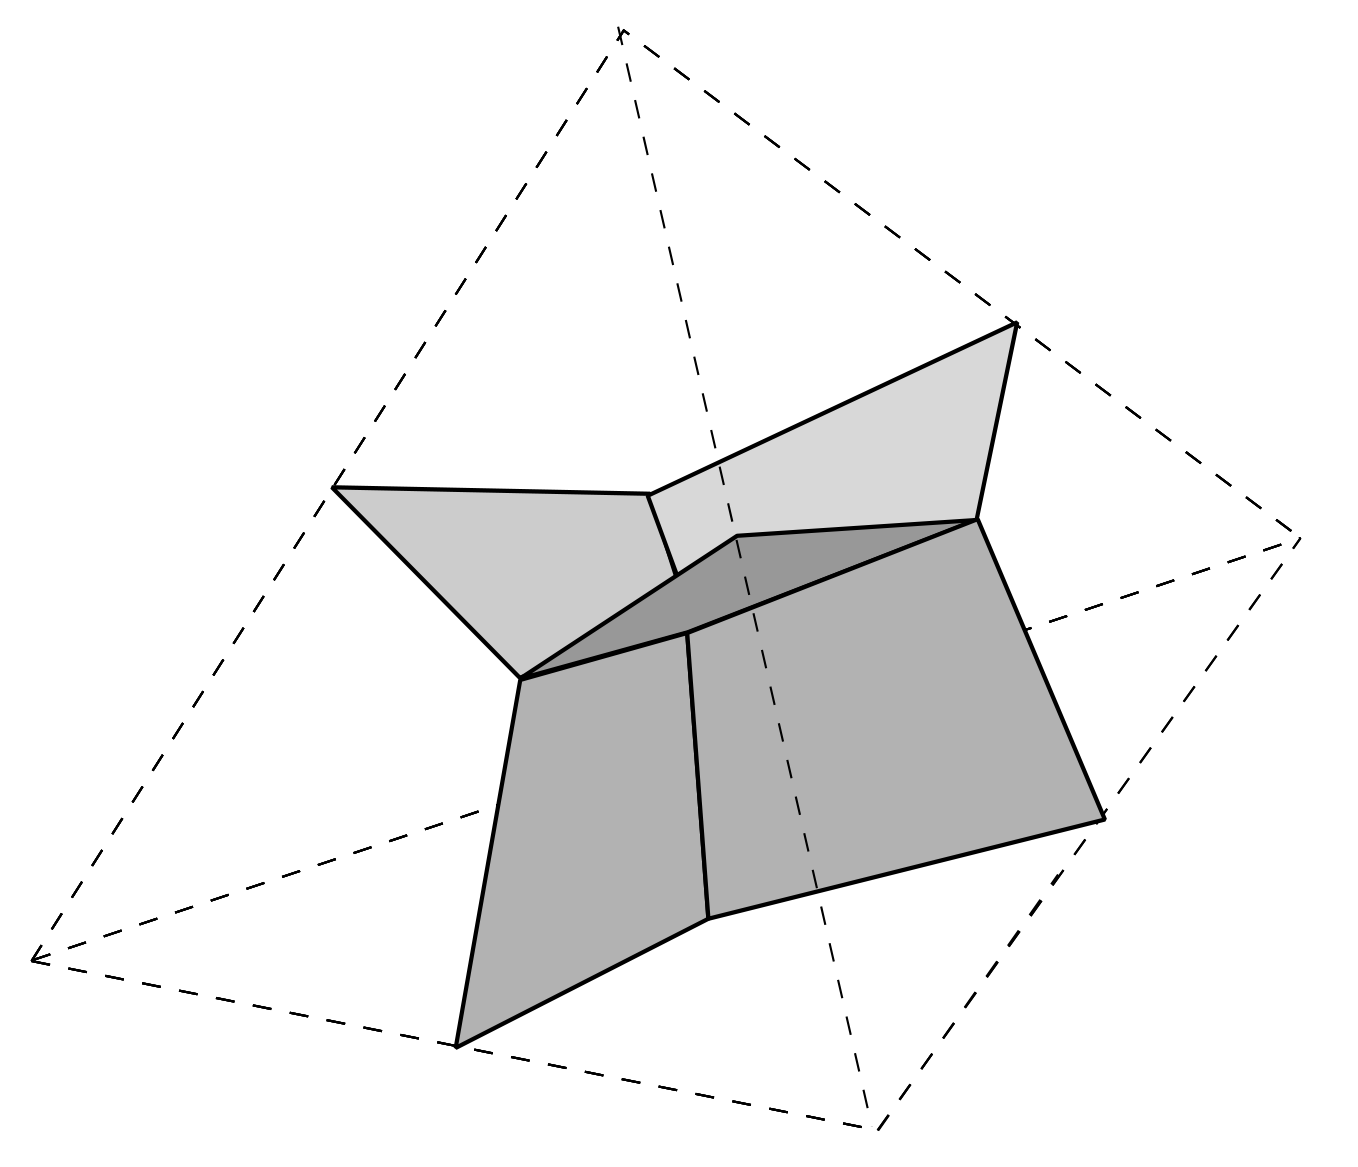
\includegraphics[width=0.5\textwidth]{figures/dual_face.png}
			\caption[单复形和对偶面]{单复形和对偶面,图片来源于\cite{Baez1999} 中的第23页}\label{pic-dual_face}
		\end{figure}

	\section{三维欧式引力:Ponzano-Regge 模型}

		早期的 spinfoam 模型是由 Ponzano 和 Regge 于1968 年提出\cite{Regge1968},并由 Turaev 和 Viro 在 1992 年的工作完善\cite{Turaev1992}。它基于 \cite{Regge1968} 中发现的如下渐进表达式
		\begin{equation}
			\left\{ \mqty{j_1&j_2&j_3\\j_4&j_5&j_6} \right\} \simeq \frac{\gkappa^{3/2}}{\sqrt{-48\uppi \ii V}} \e{\frac{\ii}{\hbar} S} + \text{c.c.} \qc \text{for large $\left\{ j_i\right\}$},
		\end{equation}
		其中左边是 Wigner 6-$j$ 符号,6个 $j$ 被标记在 Regge calculus 中的一个四面体的6条边,每条边的边长和相应的 $j$ 的关系设定为
		\begin{equation}
			l_i = \left( j_i + \frac{1}{2} \right) \gkappa \hbar,
		\end{equation}
		右边 $V$ 是四面体的体积,是 $l_i$ 的函数;$S$ 是3维欧式引力在单个四面体上的 Regge 作用量,也是 $l_i$ 的函数。在 $j_i$ 有限时此式的近似程度也非常好,如图~\ref{pic-PR_approx} 所示。
		\begin{figure}[htbp!]
			\centering
			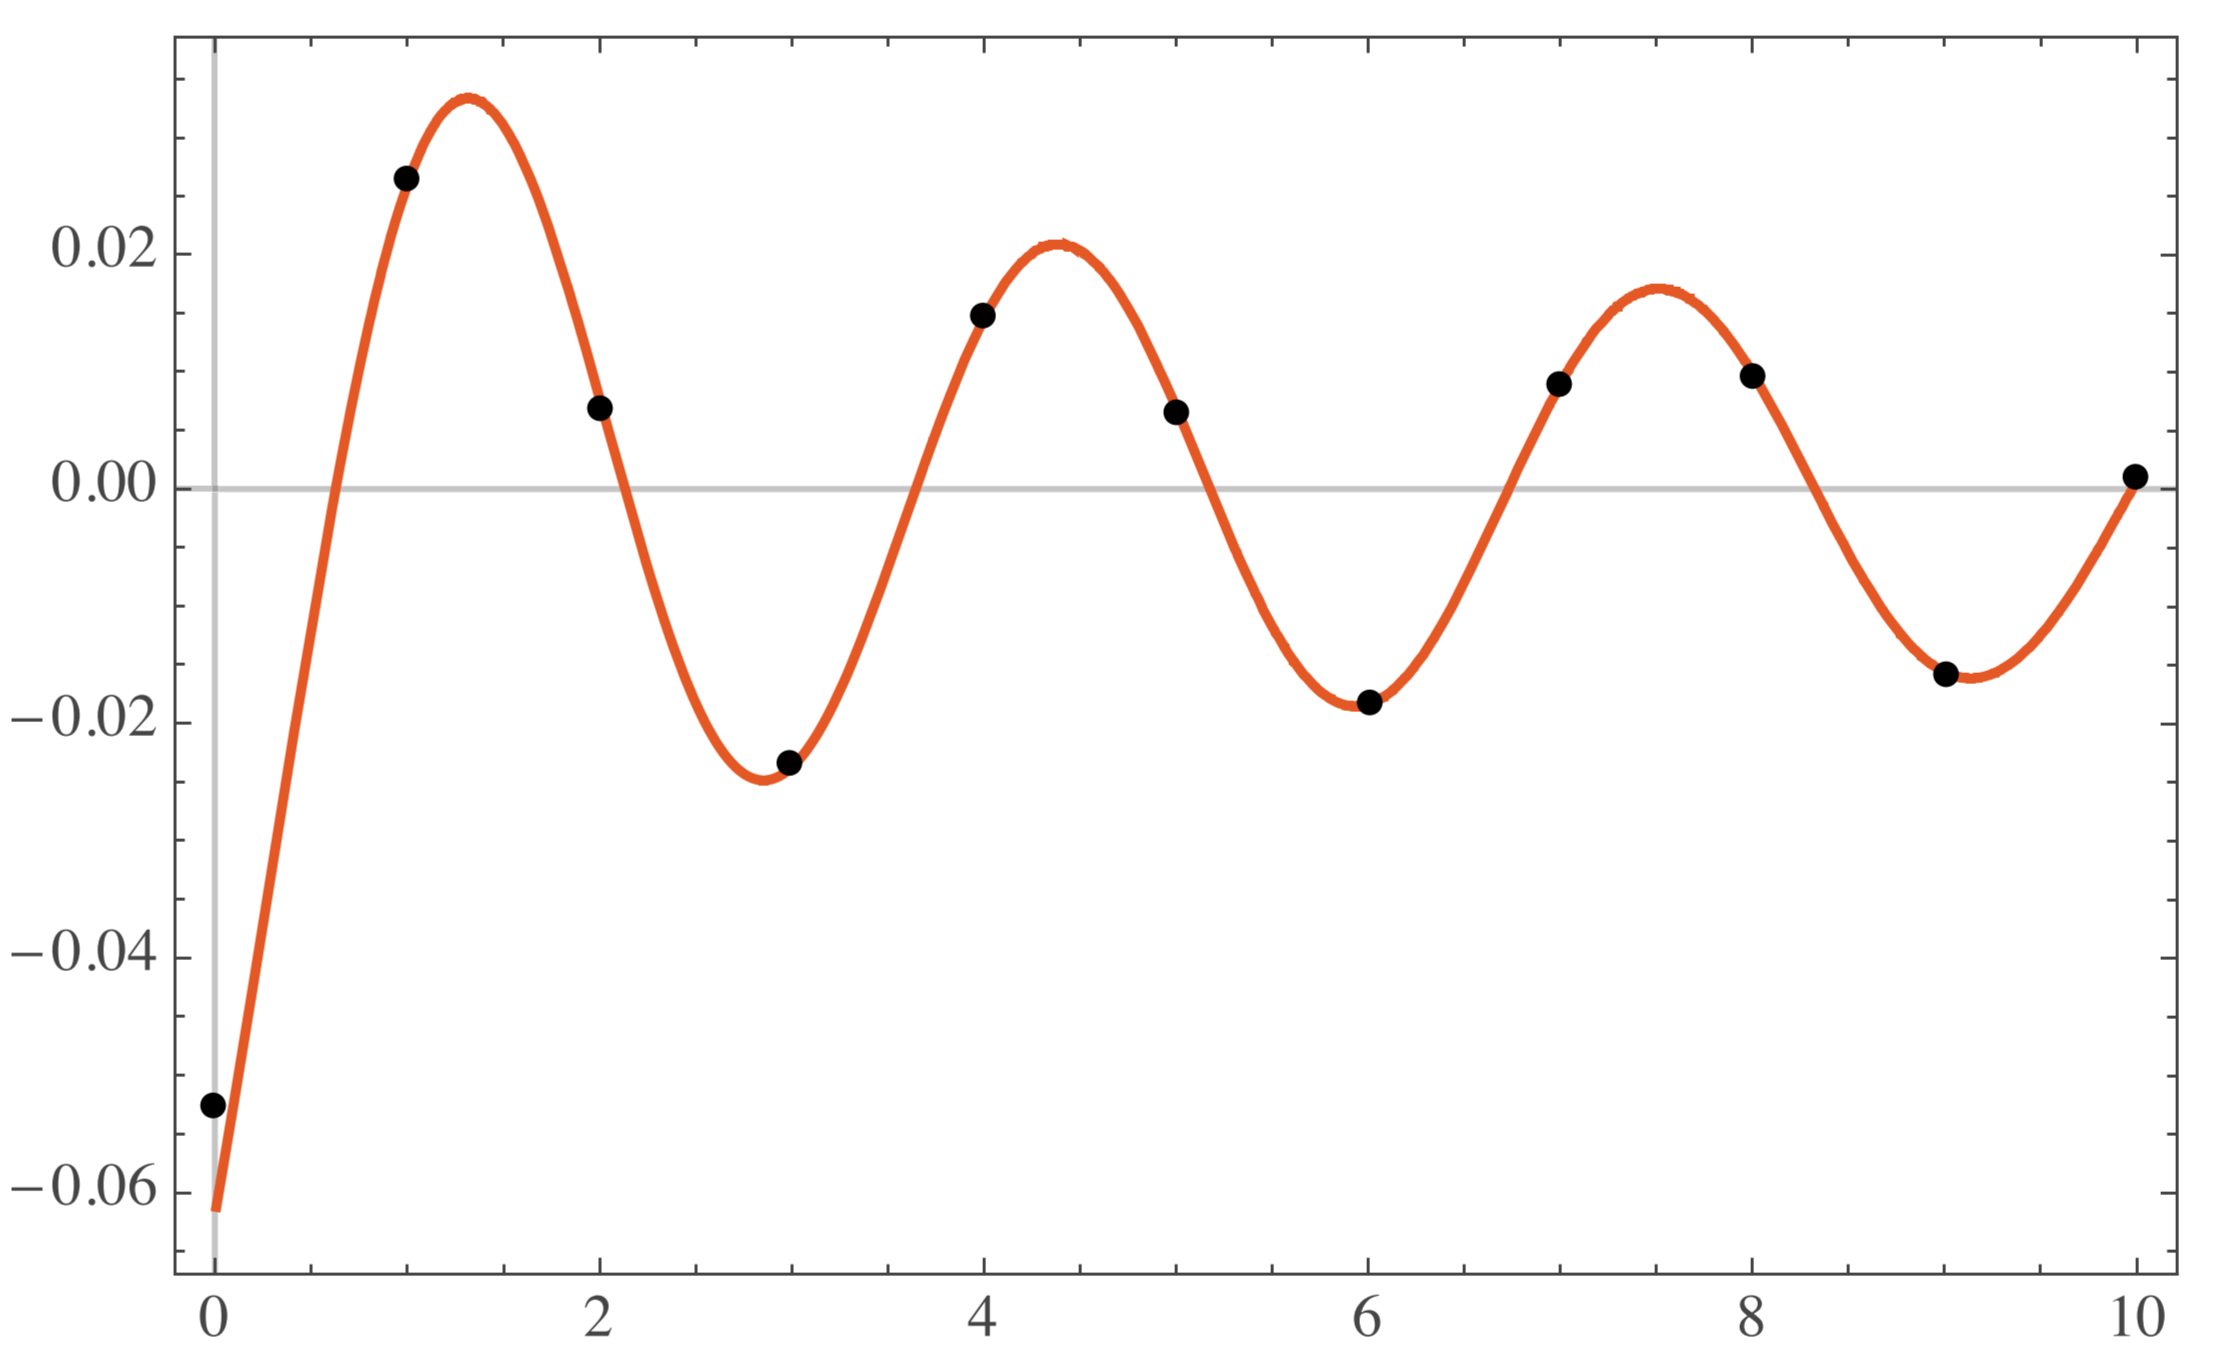
\includegraphics[width=0.5\textwidth]{figures/PRapproximate.png}
			\caption[Ponzano-Regge 近似]{$\left\{ \mqty{9&9&9\\9&9&j} \right\}$ (点)与 Ponzano-Regge 近似(线)的对比,图片引自\cite{Bianchi2017}}\label{pic-PR_approx}
		\end{figure}

		Ponzano 和 Regge 定义了“sum over 3-geometry” ,即 PR model 为:给定3维欧式时空的三角剖分 $\complex{K}$,对每个四面体 $v$ 的每个边 $f$ (记为 $f$ 是因为对应对偶面)都标记一个半整数自旋量子数 $j_f$,则其对偶复形带上这些量子数称为一个 spinfoam,并定义 PR 振幅
		\begin{equation}
			Z_{\text{PR}}(\complex{K}) = \sum_{j_f} \prod_{f} \left( 2j_f + 1 \right) \prod_{v} \left\{ 6j\right\}_v,
		\end{equation}
		可以将此式看作 Regge gravity 的路径积分表述,因而是~\eqref{eq-GR_path_integral} 的离散化版本。

		PR 模型的4维类比在近些年才有了很大的发展,4维引力的 spinfoam amplitude 具有以下的一般形式
		\begin{equation}
			Z = \sum_{j_f,i_e} \left( \prod_f \left( 2j_f + 1 \right) \right) \prod_{v} A_v(j_e,j_v),
		\end{equation}
		其中 $A_v$ 称为顶点振幅。$A_v$ 有不同的表达式,如 Freidel-Krasnov 模型\cite{Freidel1999,Freidel:2007py},Barrett-Crane 模型\cite{Barrett1998},EPRL(Engle-Pereira-Rovelli-Livine四个人的缩写) 模型\cite{EPRL2008} 等,其中 EPRL 模型是近年来普遍认为较为成功的模型。它可以以如下方式理解:将广义相对论视为带约束的 BF 理论。

	\section{BF 理论与引力}

			考虑一个4维整体双曲时空 $M = \mathbb{R} \times \spc$,定义以 $\SO{3,1}$ 为规范群的 BF 理论为
			\begin{equation}
				S_{\mathrm{BF}}[B,\omega] = \int_M \tensor{B}{_a_b^I^J} \wedge \tensor{F}{_c_d_I_J},\label{eq-BF_action}
			\end{equation}
			其中 $\tensor{B}{_a_b^I^J}$ 是在 $\SO{3,1}$ 的伴随表示中取值的二形式,$\tensor{\omega}{_a^I_J}$ 是之前定义的联络一形式,而 $\tensor{F}{_a_b_I^J}$ 是 $\tensor{\omega}{_a^I_J}$ 的曲率二形式。这个理论除了明显具有微分同胚不变性外,还具有局域规范不变性:由于 Bianchi 恒等式,作用量在变换
			\begin{equation}
				\tensor{B}{_a_b^I^J} \mapsto \tensor{B}{_a_b^I^J} + \tensor{D}{_a} \tensor{\Lambda}{_b^I^J}\label{eq-BF_gauge}
			\end{equation}
			下不变,但~\eqref{eq-BF_action} 的运动方程为
			\begin{equation}
				\tensor{F}{_a_b_I^J}=0 \qc \tensor{D}{_a} \tensor{B}{_b_c^I^J} =0,
			\end{equation}
			则所有满足运动方程的 $\tensor{B}{_a_b^I^J}$ 局域具有 $\tensor{D}{_a} \tensor{\Lambda}{_b^I^J}$ 的形式,故均规范等价于 $0$,而 $F=0$ 意味着时空几何微分同胚等价于闵氏时空,于是 BF 理论是一个拓扑场论,没有任何局域的物理自由度。

			回顾引力的 Holst 作用量~\eqref{eq-Holst_action}
			\begin{equation}
				S_{\text{Holst}}[e,\omega] = \frac{1}{2\gkappa} \int_M \frac{1}{2} \tensor{\vol}{_I_J_K_L} \tensor{e}{^I_a} \wedge \tensor{e}{^J_b} \wedge \tensor{F}{_c_d^K^L} - \frac{1}{\beta} \tensor{e}{^I_a} \wedge \tensor{e}{^J_b} \wedge \tensor{F}{_c_d_I_J},
			\end{equation}
			可以发现若记
			\begin{equation}
				\tensor{B}{_a_b^I^J} = \frac{1}{2\gkappa} \left( \frac{1}{2} \tensor{\vol}{_I_J_K_L} \tensor{e}{^I_a} \wedge \tensor{e}{^J_b} - \frac{1}{\beta} \tensor{e}{^I_a} \wedge \tensor{e}{^J_b} \right),\label{eq-B_of_e}
			\end{equation}
			则 Holst 作用量和 BF 作用量具有相同形式,但 $\tensor{B}{_a_b^I^J}$ 不能任意取值,打破了~\eqref{eq-BF_gauge} 的规范不变性,也削弱了对 $B$ 变分所得的 $F$ 的运动方程,故引力具有局域物理自由度。从~\eqref{eq-B_of_e} 反解得
			\begin{equation}
				\tensor{e}{^I_a} \wedge \tensor{e}{^J_b} = \tensor{\Sigma}{_a_b^I^J} \definedby -2\gkappa \frac{\beta^2}{1+\beta^2} \left( \frac{1}{2} \tensor{\vol}{^I^J_K_L} \tensor{B}{_a_b^K^L} + \frac{1}{\beta} \tensor{B}{_a_b^I^J} \right),\label{eq-e_of_B}
			\end{equation}
			则约束:“$\tensor{\Sigma}{_a_b^I^J}$ 必须具有 $\tensor{e}{^I_a} \wedge \tensor{e}{^J_b}$ 的形式(即,是simple 2-form)”被称为 simplicity 约束。总而言之,对 BF 理论的位型空间加上 simplicity 约束,即得到引力理论。

	\section{BF 理论的 spinfoam 量子化}

			\label{sec-BF_spinfoam}
			我们先考虑 BF 理论的离散形式的路径积分量子化。为了避免数学困难,本节考虑的是紧致规范群的 BF 理论。写出配分函数
			\begin{equation}
				Z = \int \mathcal{D}B \,\mathcal{D}\omega \, \e{\ii S_{\text{BF}}} = \int \mathcal{D} \omega \, \delta[F(\omega)],\label{eq-BF_path_integral}
			\end{equation}
			其中已略去 $\hbar$,并利用了运动方程。若用单复形 $\complex{K}$ 将时空三角剖分,并对对偶复形 $\complex{K}^*$ 中的每一对偶面 $f$ 定义
			\begin{equation}
				\tensor*{B}{_f^I^J} \definedby \int_{t_f} \tensor{B}{_a_b^I^J},
			\end{equation}
			其中 $t_f$ 是与 $f$ 对偶的 2 维单形,并对每一对偶边 $e$ 定义 holonomy $g_e$,并记 $U_f = g_{e_1} \cdots g_{e_n}$ 是绕 $f$ 的 holonomy,可以证明~\eqref{eq-BF_path_integral} 被离散化为
			\begin{equation}
				Z(\complex{K}) = \int \prod_{e\in \complex{K}^*} \dd{g_e} \prod_{f\in \complex{K}^*} \dd{B_f} \e{\ii B_f U_f} = \int \prod_{e\in \complex{K}^*} \dd{g_e} \prod_{f\in \complex{K}^*} \delta(g_{e_1} \cdots g_{g_n}),\label{eq-BF_discrete_path_integral}
			\end{equation}
			由 Peter-Weyl 定理可知
			\begin{equation}
				\delta(g) = \sum_{\rho} d_\rho \tr(\rho(g)),
			\end{equation}
			其中 $\rho$ 取遍规范群的不可约表示,$d_\rho$ 表示故~\eqref{eq-BF_discrete_path_integral} 可表示为
			\begin{equation}
				Z(\complex{K}) = \sum_{\left\{ \rho_f \right\}} \int \prod_{e\in \complex{K}^*} \dd{g_e} \prod_{f\in \complex{K}^*} d_{\rho_f} \tr(\rho_f(g_{e_1} \cdots g_{e_n})),
			\end{equation}
			此式称为 BF 理论的 spinfoam 量子化,常见于格点规范场论的教材。每个对偶面标记了 $\rho_f$ 的对偶复形称为 spinfoam,此式即是对同一三角剖分的 spinfoam 求和。

		\section{经典spinfoam引力}

			考虑对时空作三角剖分 $\complex{K}$,并记 $\complex{K}_k$ 是 $\complex{K}$ 中维度不超过 $k$ 的单形组成的子集,则 $\complex{K}_k$ 也是单复形,称为 $\complex{K}$ 的 $k$ 维骨架。

			注意到二维流形上所有二形式自动是 simple form,可考虑在 $\complex{K}_2$ 上施加约束,这和 Regge calculus 相符,即把曲率集中在2维面上,而其他地方平坦。具体来说,考虑如下作用量
			\begin{equation}
				S_{\text{classical}}[B,\omega,\lambda] \definedby \int_{M} \tensor{B}{_a_b^I^J} \wedge \tensor{F}{_c_d_I_J} + \int_{\abs{\complex{K}_2}} \tensor{\lambda}{_I} \tensor{t}{_I} \tensor{\Sigma}{_a_b^I^J},\label{eq-classical_spinfoam_action}
			\end{equation}
			其中 $\tensor{\lambda}{_I}$ 是拉氏乘子,$\tensor{t}{^I}$ 是内部空间中的一个类时矢量。对 $\tensor{\lambda}{_I}$ 的变分得到在 $\abs{\complex{K}_2}$ 上 $\tensor{t}{_I} \tensor{\Sigma}{_a_b^I^J} = 0$,则 $\tensor{\Sigma}{_a_b^I^J} = \tensor{e}{^I_a} \wedge \tensor{e}{^J_b}$ 在 $\complex{K}_2$ 上是类空的面积元。使用 $\tensor{t}{^I}$ 可将 $\tensor{B}{_a_b^I^J}$ 分解为对偶“磁场”部分和对偶“电场”部分:
			\begin{equation}
				\tensor{B}{^I_a_b} \definedby \tensor{B}{_a_b^I^J} \tensor{t}{_J} \qc \tensor{E}{^I_a_b} \definedby \frac{1}{2} \tensor{\vol}{^I^J^K^L} \tensor{B}{_a_b_J_K} \tensor{t}{_L},
			\end{equation}
			则 simplicity 约束 $\tensor{t}{_J} \tensor{\Sigma}{_a_b^I^J} = 0$ 等价于线性约束
			\begin{equation}
				\tensor{B}{^I_a_b} = - \beta \tensor{E}{^I_a_b} \qq{on} \abs{\complex{K}_2},\label{eq-linear_constraint}
			\end{equation}
			这个表达形式将在量子理论的定义中发挥重要作用。

			对~\eqref{eq-classical_spinfoam_action} 变分,在 $M' \definedby M- \abs{\complex{K}_2}$ 上如同BF 理论一样得到平庸解,但 $\abs{\complex{K}_2}$ 上则存在曲率。展示这种曲率的一种好方法是考察 loop,流形 $M'$ 是处处局部平坦的道路连通空间,但不是单连通的,因为挖去了一些二维面,绕这些面的 loop 可具有非平凡的 holonomy,并且由于局部平坦,互相同伦等价的loop 具有相同的 holonomy,于是 holonomy 实际上是定义在基本群 $\pi_1(M')$ 上的\footnote{因此,Rovelli 等提出 spinfoam gravity 可视为一种带有拓扑缺陷的拓扑场论\cite{Rovelli2011,Rovelli2010}。}。这是对偶复形派上用场的地方,每个对偶面 $f\in \complex{K}^*$ 的边缘 $\partial f = (e_1 \cdots e_n)$ 就是这样的回路,且它们生成基本群 $\pi_1(M')$。换言之,所有 $\partial f$ 上的 holonomy 即完全携带了所有曲率的信息,而且是规范不变的。至于 $\tensor{B}{_a_b^I^J}$ 的规范不变信息,可以用flux:
			\begin{equation}
				\tensor*{B}{_f^I^J} \definedby \int_{t_f} \tensor{B}{_a_b^I^J},
			\end{equation}
			其中 $t_f$ 是与 $f$ 对偶的2-单形。标记了 holonomy $g_e$ 和 flux $\tensor*{B}{_f^I^J}$ 的 2维复形 $\complex{K}^*_2$ 称为一个 foam。

		\section{\texorpdfstring{$\SL{2,\mathbb{C}}$}{SL(2,C)} 的不可约酉表示}

			由于第\ref{sec-BF_spinfoam}节的启发,这一节先简要介绍 $\SL{2,\mathbb{C}}$ ,即 $\SO{3,1}$ 的双覆盖群的不可约酉表示。更多的相关数学可参考\cite{Martin-Dussaud2019}。

			首先,在量子力学及之前关于 spin-network state 的讨论中已经遇到 $\SU{2}$ 的所有不可约酉表示,即 spin-$j$ 表示,但这里为了方便及与文献一致而稍稍改变记号,将表示空间 $\Hil_j$ 上的三个角动量算符记为 $L^i$,$i=1,2,3$,有
			\begin{equation}
				\left[ L^i, L^j \right] = \ii \tensor{\vol}{^i^j_k} L^k,
			\end{equation}
			$\Hil_j$ 上的一组基底为 $\ket{j,m}$。

			$\sll{2,\mathbb{C}}$ 等于 $\su{2} \oplus \ii\, \su{2}$,故其表示可由 $\SU{2}$ 的表示构建。记六个洛伦兹生成元为 $\tensor{J}{^I^J}$,则可定义旋转生成元
			\begin{equation}
				\tensor{L}{^I} = \frac{1}{2} \tensor{\vol}{^I_J_K_L} \tensor{J}{^J^K} \tensor{t}{^L},
			\end{equation}
			及 boost 生成元
			\begin{equation}
				\tensor{K}{^I} = \tensor{J}{^I^J} \tensor{t}{_J},
			\end{equation}
			它们都是空间矢量,可投影为 $\tensor{L}{^i}$ 和 $\tensor{K}{^i}$,对易关系为
			\begin{equation}
				\begin{split}
					\left[ \tensor{L}{^i}, \tensor{L}{^j} \right] &= \ii \tensor{\vol}{^i^j_k} \tensor{L}{^k},\\
					\left[ \tensor{L}{^i}, \tensor{K}{^j} \right] &= \ii \tensor{\vol}{^i^j_k} \tensor{K}{^k},\\
					\left[ \tensor{K}{^i}, \tensor{K}{^j} \right] &= - \ii \tensor{\vol}{^i^j_k} \tensor{K}{^k}.
				\end{split}
			\end{equation}

			$\SL{2,\mathbb{C}}$ 的无穷维不可约酉表示的 principal series $\rho^{(p,j)}$ 定义在 $\Hil^{(p,j)} = L^2(\mathbb{C})$ 上,内积为
			\begin{equation}
				\left\langle f, f' \right\rangle = \frac{\ii}{2} \int_{\mathbb{C}} \overline{f(z)} f'(z) \dd{z} \dd{\bar{z}},
			\end{equation}
			而 $a = \mqty(a_{11} & a_{12} \\ a_{21} & a_{22})$ 的作用定义为
			\begin{equation}
				\left( \rho^{(p,j)}(a) f \right)(z) \definedby \left( a_{11} z + a_{22} \right)^{\ii p+j-1} \overline{\left( a_{11} z + a_{22} \right)}^{\ii p-j-1} f\left( \frac{a_{11}z+a_{21}}{a_{12}z +a_{22}} \right),
			\end{equation}
			其中 $p$ 是实数,$j$ 是半整数。$\rho^{(p,j)}$ 和 $\rho^{(-p,-j)}$ 等价,故不妨限制 $p,j \geqslant 0$。这个表示看起来很复杂,但它具有分解
			\begin{equation}
				\Hil^{(p,j)} = \Hil_j \oplus \Hil_{j+1} \oplus \Hil_{j+2} \oplus \cdots,
			\end{equation}
			其中 $\Hil_{j'}$ 是 $L^2$ 的本征子空间,也是熟知的 $\SU{2}$ 的表示空间,故 $\Hil^{(p,j)}$ 有正交归一基底
			\begin{equation}
				\left\{ \ket{(p,j);j',m} \in \Hil^{(p,j)} \,\middle|\, j' \in \left\{ j,j+1,\cdots \right\} , m\in \left\{ -j',-j'+1, \cdots , j' \right\} \right\},
			\end{equation}
			并可定义线性映射 $Y$ map
			\begin{equation}
				Y_\beta \colon \bigoplus_j \Hil_j \rightarrow \bigoplus_j \Hil^{(\beta(j+1),j)} \qc \ket{j,m} \mapsto \ket{(\beta(j+1),j);j,m},
			\end{equation}
			它具有以下重要性质
			\begin{equation}
				\mel{j,m}{Y_\beta^\dagger \left( \tensor{K}{^i} + \beta \tensor{L}{^i} \right) Y_\beta}{j,m'} = 0 \qc \forall m,m',
			\end{equation}
			换句话说,$\tensor{K}{^i} + \beta \tensor{L}{^i}$ 在 $Y_\beta$ 的像 $\Hil_\gamma \definedby \image{Y_\beta}$ 上为零。

		\section{边界态及LQG}

			现在工具已经准备完毕,可以着手考虑跃迁振幅了。首先需要考虑边界,设四维时空区域 $D$ 有三维边界 $\partial D$,则 $D$ 的剖分 $\complex{K}$ 诱导出 $\partial D$ 的分解 $\complex{K}^{(3)}$。考虑线性约束,则辛形式 $\updelta \tensor{B}{_a_b^I^J} \wedge \updelta \tensor{\omega}{_c_I_J}$ 可约化为 $\updelta \tensor{E}{_a_b^I} \wedge \updelta \tensor{A}{_c_I}$,其中 $\tensor{E}{_a_b^I}$ 是之前定义的对偶“电场”,而
			\begin{equation}
				\tensor{A}{_a^I} = \frac{1}{2} \tensor{\vol}{^I^J^K^L} \tensor{\omega}{_a_J_K} \tensor{t}{_L} + \beta \tensor{\omega}{_a^I^J} \tensor{t}{_J}
			\end{equation}
			是实 Ashtekar 变量。并且,固定 $\tensor{t}{^I}$ ,则规范群约化为 $\SO{3}$,于是我们又回到了正则圈量子引力理论的起点。注意到对偶2-复形 $\complex{K}^*_2$ 在 $\partial D$ 上诱导一个一维复形,即图 $\gamma = \left(\complex{K}^{(3)}\right)^*$,其中每个顶点改称为 节点(node)$n$ 对偶于四面体,每个连线(link)$l$ 对偶于一个三角形。每个节点 $n$ 是某条对偶边 $e$ 与 $\partial D$ 的交点,而每条连线 $l$ 是某个对偶面 $f$ 与 $\partial D$ 的交线。记每条连线 $l$ 的 holonomy 为 $h_l$,每个2-单形 $t_l$ 的“电”通量为
			\begin{equation}
				L^i_l = \int_{t_l} \tensor{E}{_a_b^i},
			\end{equation}
			则再次得到了 holonomy-flux 代数。

			在 spinfoam 引力中,除了 $L^i_f$ 外还有另一个通量,即“磁”通量
			\begin{equation}
				K^i_l = \int_{t_l} \tensor{B}{_a_b^i},
			\end{equation}
			线性约束为
			\begin{equation}
				\myvec{K}_l = \beta \myvec{L}_l.
			\end{equation}
			使用 $Y$ 映射,可将正则圈量子引力的 $\Hkin$ 的 spin-network 分解中的每一个 $\Hil_j$ 替换为 $\Hil^{(\beta(j+1),j)}$,例如对于 $L^2(\SU{2},\mu_H)$,$Y_\beta$ 在其上有诱导映射 $L^2(\SU{2},\mu_H) \rightarrow L^2(\SL{2,\mathbb{C}},\mu_H)$:
			\begin{equation}
				\tensor{D}{^j_m_n}=\mel{j,m}{\rho^j(\cdot)}{j,n} \mapsto \tensor{D}{^{(\beta(j+1),j)}_{jm jn}}=\mel{j,m}{Y^\dagger_\beta \rho^{(\beta(j+1),j)}(\cdot)Y_\beta}{j,n},
			\end{equation}
			则每个定义在 $\bar{\configurationspace{A}}_\gamma = \SU{2}^L$ 上的 spin-network state $\psi_{j_l,i_n}$ 可被映射为 $\SL{2,\mathbb{C}}^L$ 上的:
			\begin{equation}
				\psi_{j_l,i_n}(\{g_l\}) \mapsto \operatorname{C} \left( \bigotimes_{n\in N(\gamma)} Y_\beta i_n \bigotimes_{l\in L(\gamma)} \rho^{(\beta(j+1),j)}(g_l) \right),
			\end{equation}
			不过这并不是 $\SL{2,\mathbb{C}}$ 规范不变的,还需作规范群平均
			\begin{equation}
				P_{\SL{2,\mathbb{C}}} \psi(\left\{ g_l\right\}) \definedby \int_{\SL{2,\mathbb{C}}^N} \prod_{n} \dd{g_n} \psi\left( \left\{ g_{s(l)} g_l g_{t(l)}^{-1} \right\} \right),
			\end{equation}
			于是可定义 $f_\beta \definedby P_{\SL{2,\mathbb{C}}} \circ Y_\beta$ ,得到
			\begin{equation}
				\psi^\beta_{j_l,i_n} \definedby f_\beta \psi_{j_l,i_n},
			\end{equation}
			这组基底下 $\tensor*{K}{^i_l} + \beta \tensor*{L}{^i_f}$ 的矩阵元总为零,故线性约束得解。

		\section{spinfoam 配分函数与跃迁振幅}

			回忆之前第\ref{sec-BF_spinfoam}节中 BF 理论的 spinfoam 量子化,
			\begin{equation}
				\begin{split}
					Z(\complex{K}) &= \sum_{\left\{ \rho_f \right\}} \int \prod_{e\in \complex{K}^*} \dd{g_e} \prod_{f\in \complex{K}^*} d_{\rho_f} \tr(\rho_f(g_{e_1} \cdots g_{e_n}))\\
					&= \int \prod_{e\in \complex{K}^*} \dd{g_e} \prod_{f\in \complex{K}^*} \sum_{\rho_f} d_{\rho_f} \tr(\rho_f(g_{e_1} \cdots g_{e_n}))\\
					&= \int \prod_{e\in \complex{K}^*} \dd{g_e} \prod_{f\in \complex{K}^*} \amplitude^{\text{BF}}_f(\{g_e\}),
				\end{split}
			\end{equation}
			在洛伦兹群的情况下,每个对偶面贡献一个面振幅
			\begin{equation}
				\amplitude^{\text{BF}}_f(\{g_e\}) = \delta \left( \prod_{e\in \partial f} g_e \right) = \sum_{k=0,\frac{1}{2},\cdots} \int_0^\infty \dd{p} \left( p^2 + k^2 \right) \tr(\prod_{e\in \partial f} \rho^{(p,k)}(g_e)),
			\end{equation}
			为了得到引力,需要添加线性约束。经过前面的讨论,线性约束相当于把右边的表示 $\Hil^{(p,k)}$ 换为 $\Hil_\beta = \image{Y_\beta}$,单个面振幅修改为
			\begin{equation}
				\amplitude_f(\{g_e\}) = \sum_{j} (2j+1) \tr(\prod_{e\in \partial f} Y^\dagger_\beta \rho^{(\beta(j+1),j)}(g_e) Y_\beta),
			\end{equation}
			其中 $\tr$ 是在 $\Hil_j$ 上取的。于是,加上边界后,考虑到固定边界连线 $l$ 上的 holonomy $g_l$,有跃迁振幅
			\begin{equation}
				W_{\complex{K}^*}(\{g_l\}) = \int \dd{g_e} \prod_{f\in \complex{K}^*} \amplitude_f(\{g_e\}),
			\end{equation}
			如同正则圈量子引力中所做的一样,可以在对偶边$e$上重新耦合 $\Hil_{j_f}$,这里略去过程,结果为\cite{Rovelli2011}
			\begin{equation}
				W_{\complex{K}^*}\left(\left\{ j_l \right\},\left\{ i_n \right\}\right) \definedby \sum_{\left\{ j_f \right\},\left\{ i_e \right\}} \prod_{f\in \complex{K}^*} \left( 2j_f +1 \right) \prod_{v \in \complex{K}^*} \amplitude_v(j_f,i_e),
			\end{equation}
			其中顶点振幅
			\begin{equation}
				\amplitude_v(j_f,i_e) \definedby \tr(\bigotimes_{e\in v} f_\beta i_e),
			\end{equation}
			这里 $\tr$ 要按 $\Hil_{j_f}$ 互相缩并。这个顶点振幅还有一个有趣的表达式,设我们把与 $v$ 对偶的4-单形 $\Delta_v$ 的边界与 $v$ 周围的 $f$ 和 $e$ 相交的 $l$、$n$ 视为一个图,将 $j_f$,$i_e$ 对应标在 $l$ 和 $n$ 上得到一个 spin-network state $\psi_v$,则有
			\begin{equation}
				\amplitude_v(\psi_v) = (f_\beta \psi_v)(\{g_l=\II\}),
			\end{equation}
			其中 $\II$ 是 $\SL{2,\mathbb{C}}$ 的单位元。我们将引力视为了带 simplicity 约束的 局部平直 BF 理论,这里约束体现在 $f_\beta$,而局部平直体现在平凡的 holonomy $\{g_l = \II\}$。

			最后,注意到要使我们推导的出发点~\eqref{eq-classical_spinfoam_action} 真正成为 Holst 作用量,需使剖分 $\complex{K}$ 不断加密,或取遍各种剖分,以使得 simplicity 约束处处成立。于是可定义完整跃迁振幅是剖分加密下的极限
			\begin{equation}
				W = \lim_{\complex{K}} W_{\complex{K}},\label{eq-continuous_limit}
			\end{equation}
			或对各种剖分求和
			\begin{equation}
				W = \sum_{\complex{K}} W^*_{\complex{K}},\label{eq-sum_over_complex}
			\end{equation}
			其中两种方法中右端的 $\complex{K}$ 都要固定其边界诱导的图 $\complex{K}^*_1$,并且~\eqref{eq-sum_over_complex} 中 $W^*$ 表示要将 $j=0$ 从求和中剔除,并为不同的添加适当的权重因子。两式实际上是等价的,参见 \cite{Rovelli:2010qx}。于是,若考虑夹在两片类空超曲面 $\Sigma,\Sigma'$ 间的区域 $D$,如图~\ref{pic-D},则固定边界上的 spin-network 后 $W$ 给出了边界上的 spin-network 态 $\psi_s,\psi_{s'}$ 之间的跃迁振幅,即给出了在正则圈量子引力中较为复杂的物理内积
			\begin{equation}
				\ip{\psi_s}{\psi_{s'}}_{\text{phys}} = W\left(\left\{ j_l \right\},\left\{ i_n \right\};\left\{ j_{l'}\right\},\left\{ i_{n'} \right\}\right).
			\end{equation}
			\begin{figure}[htbp!]
				\centering
				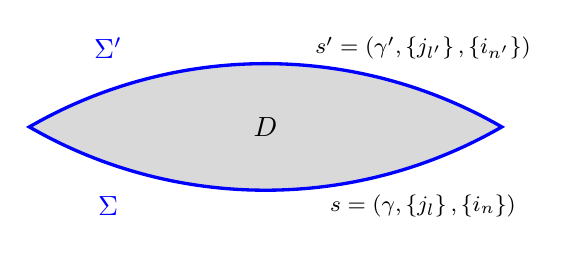
\begin{tikzpicture}
					\draw[very thick,blue,fill=gray,fill opacity=0.3] (3,0) -- (3,0) arc (60:120:6) -- (-3,0) -- (-3,0) arc (240:300:6) -- cycle;
					% \draw[very thick,blue](-3,0) arc (240:300:6);
					\node (Sigma) at (-2,-1) {\color{blue} $\Sigma$};
					\node (Sigma') at (-2,1) {\color{blue} $\Sigma'$};
					\node (D) at (0,0) {$D$};
					\node (s) at (2,-1) {\footnotesize $s=\left(\gamma,\left\{ j_l \right\},\left\{ i_n \right\}\right)$};
					\node (s') at (2,1) {\footnotesize $s'=\left(\gamma',\left\{ j_{l'} \right\},\left\{ i_{n'} \right\}\right)$};
				\end{tikzpicture}
				\caption{夹在两片类空超曲面 $\Sigma,\Sigma'$ 间的区域 $D$}\label{pic-D}
			\end{figure}

		\section{相干态表示}

			上一节中得到的跃迁振幅,其边界态是用量子的 spin-network 表示的,但物理上考虑,边界应赋半经典态,即第\ref{chp-application}章第\ref{sec-coherent_states}节 中定义的 相干态。为此,先注意到当 $i_e$ 取 LS coherent intertwiner $i_e=i_e(\{\myvec{n}_{fe}\})$ 时,在 $\Delta_v$ 的边界上诱导一个 LS 态 $\psi_v$,有
			\begin{equation}
				\begin{split}
					\amplitude_v(j_f,\myvec{n}_{fe}) &= (f_\gamma \psi_v)(\II)\\
					&= \left( \prod_{e\in \partial v} \int_{\SL{2,\mathbb{C}}} \dd{g_{ve}} \right) Y_\beta \psi_v(\{g_{ev} g_{ve'}\})\\
					&= \left( \prod_{e\in \partial v} \int_{\SL{2,\mathbb{C}}} \dd{g_{ve}} \right) \prod_{(e,e')} \mel{j_f,\myvec{n}_{ef}}{Y_\beta^\dagger g_{ev} g_{ve'} Y_\beta}{j_f,\myvec{n}_{e'f}},
				\end{split}
			\end{equation}
			其中约定 $g_{ev} = g_{ve}^{-1}$,则对整个跃迁振幅,有
			\begin{equation}
				\begin{split}
					&W_{\complex{K}^*}\left(\left\{ j_l\right\},\left\{ \myvec{n}_{ln} \right\}\right)\\
					={}& \sum_{\left\{ j_f \right\}} \prod_{f\in \complex{K}^*} \left( 2j_f + 1 \right) \prod_{\substack{(v,e)\\v\in e}} \int_{\SL{2,\mathbb{C}}} \dd{g}_{ve} \prod_{\substack{(e,f)\\e\in f}} \int_{S^2} \dd{\myvec{n}_{ef}} \prod_{v\in f} \mel{j_f,\myvec{n}_{ef}}{Y_\beta^\dagger g_{ev} g_{ve'} Y_\beta}{j_f,\myvec{n}_{e'f}},
				\end{split}
			\end{equation}
			这就是 spinfoam 跃迁振幅的 LS 相干态表示。使用全纯相干态表示更合适,因为全纯相干态是在经典态周围的高斯波包,但稍复杂一些,结果是\cite{Bianchi2010}
			\begin{equation}
				\begin{split}
					&\amplitude_v(\{H_f,t_f\})\\
					={}& \prod_{e\in \partial v} \int_{\SL{2,\mathbb{C}}} \dd{g}_{ve} \prod_{(e,e')} \sum_{j_f} \left( 2 j_f + 1 \right) \e{-j_f(j_f+1) t_f} \tr(D^{j_f}(H_f) Y_\beta^\dagger D^{(\beta (j_f+1),j_f)}(g_{ev}g_{ve'}) Y_\beta),
				\end{split}
			\end{equation}
			其中 $D^{j}$ 是 $\SU{2}$ 上的 Wigner D矩阵在 $\SL{2,\mathbb{C}}$ 上的解析延拓。

			\nomenclature{$D^j,\tensor{D}{^j_m_n}$}{Wigner D矩阵}

		\section{半经典极限与离散几何}

			spinfoam 跃迁振幅可定义两种极限,一是~\eqref{eq-continuous_limit} 中的连续极限,二是半经典极限,如图~\ref{pic-semiclassical_limit} 所示。半经典极限对应 $\hbar\rightarrow 0$,或量子数趋于无穷。故在 spinfoam 引力中,认为半经典极限为 $j_f \rightarrow \infty$。
			\begin{figure}[htbp!]
				\centering\small
				\begin{tikzpicture}
					\node (s) at (0,0) {spinfoam 引力};
					\node (R) at (5,0) {Regge 几何};
					\node (Q) at (0,3) {完整的量子引力};
					\node (c) at (5,3) {广义相对论};
					\draw[\myarrow] (s) -- node[above]{\scriptsize 半经典极限} (R);
					\draw[\myarrow] (s) -- node[left]{\scriptsize 连续极限} (Q);
					\draw[\myarrow] (Q) -- node[above]{\scriptsize 半经典极限} (c);
					\draw[\myarrow] (R) -- node[left]{\scriptsize 连续极限} (c);
				\end{tikzpicture}
				\caption{连续极限与半经典极限}\label{pic-semiclassical_limit}
			\end{figure}

			在 \cite{Barrett2009} 中研究了单个4-单形 $\Delta_v$ 的顶点振幅 $\amplitude_v(j_l,\myvec{n}_{ln})$,结果表明,若令 $j_f \mapsto \lambda j_f$,在 $\lambda\rightarrow \infty$ 极限下,注意到根据面积算符的谱,有 $A_l \simeq \gkappa \beta j_f$,则 $\gkappa \beta j_l \myvec{n}_{ln}$ 可视为 $\Delta_v$ 边界上的四面体各面的法矢,据此计算\emph{不足角}(deficit angle) $\theta_l$,则有渐进表达式
			\begin{equation}
				\amplitude_v \simeq \frac{1}{\mathcal{N}\lambda^{12}} \e{\ii \lambda S} + \text{c.c.},
			\end{equation}
			其中 $\mathcal{N}$ 是一个系数,
			\begin{equation}
				S = \sum_{l\in \gamma_v} \beta j_l \theta_l \simeq \frac{1}{\gkappa} \sum_{l\in\gamma_v} A_l \theta_l
			\end{equation}
			渐进为 Regge 作用量。故单个4-单形的半经典极限是正确的。

			韩慕辛和张鸣一于2011年对欧式号差\cite{Han2011rf}和洛伦兹号差\cite{Han2011re}的情况分别得到了更进一步的结果,对于任意的单复形 $\complex{K}$,令 $j_f \mapsto \lambda j_f$,则 $W_{\complex{K}^*}$ 具有 $\int \dd{x} a(x) \e{\lambda S(x)}$ 的形式,$S$ 称为“spinfoam 作用量”,$x$ 代表 spinfoam 变量。对于 $\lambda \rightarrow \infty$ 极限,它渐进为 $a(x_c) \e{\lambda S(x_c)}$,其中 $x_c$ 是 $S$ 的临界点(critical point),即
			\begin{equation}
				S'(x_c) =0 \qc \text{且} \Re S(x_c) = 0,
			\end{equation}
			对 spinfoam 作用量求解临界点,结果表明,除了用 $\myvec{n}_{ef}$ 可构造各个与 $e$ 对偶的四面体 $t_e$ 的法矢$N_{ef}$外,还有相邻四面体$t_e,t_{e'}$ 的公共面 $t_f$ 处满足 $N_{ef} = N_{e'f}$,故四面体具有正确的粘合。最后,spinfoam 作用量在临界点处也具有 Regge 作用量的形式。故至此可以说 spinfoam 引力的半经典极限是 Regge 作用量,而Regge 作用量取经典极限即为广义相对论的 爱因斯坦希尔伯特作用量。

	% % !TeX root = ../main.tex

\chapter{费米子耦合}

	在之前的章节中分别建立了正则圈量子引力及 spinfoam 模型,但都是纯引力的理论,还未与物质场耦合。我们知道,除引力外,目前标准模型包括了 杨-米尔斯 规范场、费米子、希格斯玻色子。正则圈量子引力与规范群为 $G$ 的规范场耦合时只需将 Ashtekar 联络 $A$ 替换为规范群为 $\SU{2} \times G$ 的联络 $(A , A_{\text{YM}})$\cite{Rovelli2004,Thiemann2007},而 spinfoam 模型与规范场的耦合也有了很多讨论,如\cite{Alexander2011,Mikovic2002,Speziale2007mt}。正则圈量子引力耦合费米子和标量场的方法类似,是将旋量 $\psi$ 或标量 $\phi$ 标记在图的顶点上,定义扩充的柱函数\cite{Rovelli2004,Han2005,Thiemann2007},主要难点在于处理哈密顿算符。spinfoam 模型与费米子和标量场耦合的方式也相似,是将旋量或标量标记在对偶顶点 $v$ 上。本文介绍 spinfoam 模型与费米子的耦合。

	2010年Bianchi、韩慕辛、Rovelli等人首次给出了spinfoam 模型与费米子耦合的定义,但只用于2-旋量\cite{Bianchi2010bn},2011年韩慕辛和 Rovelli 定义了 spinfoam 与 狄拉克 4-旋量的耦合\cite{Han2011},本文采用后者。

	经典的狄拉克作用量为
	\begin{equation}
		S_F \definedby \int_M \frac{\ii}{2} \left( \bar{\psi} \tensor{\gamma}{^a} \tensor{D}{_a} \psi - \overline{\tensor{D}{_a} \psi} \tensor{\gamma}{^a} \psi \right) - m_0 \bar{\psi} \psi,\label{eq-Dirac_action}
	\end{equation}
	其中 $\tensor{\gamma}{^a} \definedby \tensor{\gamma}{^I} \tensor{e}{^a_I}$,而 $\tensor{D}{_\mu}$ 是旋量丛上的协变导数
	\begin{equation}
		\tensor{D}{_a} \psi = \Partial{a} \psi + \frac{1}{2} \tensor{A}{_a^I^J} \tensor{S}{_I_J} \psi,
	\end{equation}
	其中
	\begin{equation}
		\tensor{A}{_a^I^J} \definedby \tensor{\vol}{^I^J^K} \tensor{A}{_a_K}
	\end{equation}
	是对偶的 Ashtekar 联络,$\tensor{S}{^I^J} \definedby \frac{1}{4}\left[ \tensor{\gamma}{^I}, \tensor{\gamma}{^J} \right]$ 是洛伦兹群的生成元。%首先考虑对 $M$ 作三角剖分 $\complex{K}$ 后,将作用量~\eqref{eq-Dirac_action} 离散化。设旋量场离散化为每个对偶顶点 $v$ 处标记一个 $\psi_v$,我们把~\eqref{eq-Dirac_action} 分成三项,\cite{Han2011}中给出第一项的离散化为
	% \begin{equation}
	% 	S_1 = 2 \ii \sum_{e\in E(\complex{K}^*)} V_e \bar{\psi}_{s(e)} \tensor{\gamma}{^I} \tensor{n}{_I}(e) \left( G_e \psi_{t(e)} - \psi_{s(e)} \right),\label{eq-S1}
	% \end{equation}
	% 其中 $V_e$ 是与 $e$ 对偶的四面体的体积,$\tensor{n}{^I}(e) = \tensor{e}{^I_a} \tensor{n}{^a}(e)$ 是 $e$ 在 $s(e)$ 处的单位切矢,而 $G_e$ 是沿 $e^{-1}$ 的 holonomy
	% \begin{equation}
	% 	G_e \definedby \pathorder \exp(\frac{1}{2} \int_e \tensor{A}{_a^I^J} \tensor{S}{_I_J}),
	% \end{equation}
	% 现证明~\eqref{eq-S1} 的连续极限,\cite{Han2011} 原文中的证明是不太精确的,这里本文给出仔细的证明。
	% \begin{Proof}
	% 	选择这样的区域 $\Omega$,它足够小,使得场及场的导数在 $\Omega$ 上变化不大,并设 $\complex{K}$ 细分到使得 $\Omega$ 包含很多个 $\complex{K}$ 中的 4-单形 $\Delta_v$。将 $e$ 参数化为 $e(s)$,使 $\tensor{e}{^I_a} \tensor{{\dot{e}}}{^a}$ 是内部空间的单位矢量,$s\in [0,l(e)]$,则 $l(e)$ 是在连续极限下趋于零的小量,有
	% 	\begin{equation}
	% 		\begin{split}
	% 			G_e \psi_{t(e)} &\simeq \left( \II + \frac{1}{2} l(e) \tensor{n}{^a}(e) \tensor{A}{_a^I^J} \tensor{S}{_I_J} \right) \left( \psi_{s(e)} + l(e) \tensor{n}{^a}(e) \left( \Partial{a} \psi \right)_{s(e)} \right)\\
	% 			&\simeq \psi_{s(e)} + l(e) \tensor{n}{^a}(e) \left( \tensor{D}{_a} \psi \right)_{s(e)},
	% 		\end{split}
	% 	\end{equation}
	% 	故连续极限下
	% 	\begin{equation}
	% 		\begin{split}
	% 			S_1(\Omega) & \simeq 2\ii \sum_{e\in E(\complex{K}^*) \cap\, \Omega} V_e \bar{\psi}_{s(e)} \tensor{\gamma}{^I} \tensor{n}{_I}(e) l(e) \tensor{n}{^a}(e) \left( \tensor{D}{_a} \psi \right)_{s(e)}\\
	% 			& = 2\ii \sum_{e\in E(\complex{K}^*) \cap\, \Omega} V_e \bar{\psi}_{s(e)} \tensor{\gamma}{^I} \tensor{n}{_I}(e) l(e) \tensor{n}{^J}(e) \tensor{e}{^a_J}(s(e)) \left( \tensor{D}{_a} \psi \right)_{s(e)}\\
	% 			& \simeq 2\ii \bar{\psi}_{\Omega} \tensor{\gamma}{^I} \left( \tensor{D}{_a} \psi \right)_{\Omega} \tensor{e}{^a_J}(\Omega) \sum_{e\in E(\complex{K}^*) \cap\, \Omega} V_e \tensor{n}{_I}(e) l(e) \tensor{n}{^J}(e),\label{eq-S1_continuous}
	% 		\end{split}
	% 	\end{equation}
	% 	其中最后一行用到了 $\psi$ ,$\tensor{D}{_a} \psi$和 $\tensor{e}{^a_I}$ 在 $\Omega$ 内变化不大的性质。
	% 	考察
	% 	\begin{equation}
	% 		\sum_{e\in E(\complex{K}^*) \cap\, \Omega} V_e \tensor{n}{_I}(e) l(e) \tensor{n}{^J}(e),
	% 	\end{equation}
	% 	注意到它在4维转动下不变,知它正比于 $\tensor{\delta}{^J_I}$;再对 $I$,$J$ 缩并得到 $\mathrm{Vol}(\Omega)$,故
	% 	\begin{equation}
	% 		\sum_{e\in E(\complex{K}^*) \cap\, \Omega} V_e \tensor{n}{_I}(e) l(e) \tensor{n}{^J}(e) = \frac{1}{4} \mathrm{Vol}(\Omega) \tensor{\delta}{^J_I},
	% 	\end{equation}
	% 	则代入~\eqref{eq-S1_continuous} 得
	% 	\begin{equation}
	% 		S_1(\Omega) \simeq \frac{\ii}{2} \mathrm{Vol}(\Omega) \bar{\psi}_{\Omega} \tensor{\gamma}{^a} \left( \tensor{D}{_a} \psi \right)_{\Omega},
	% 	\end{equation}
	% 	对整个 $\complex{K}$ 则为
	% 	\begin{equation}
	% 		S_1 \simeq \frac{\ii}{2} \sum_{\Omega} \mathrm{Vol}(\Omega) \bar{\psi}_{\Omega} \tensor{\gamma}{^a} \left( \tensor{D}{_a} \psi \right)_{\Omega},
	% 	\end{equation}
	% 	即~\eqref{eq-Dirac_action} 的第一项。
	% \end{Proof}

	% 第二项为复共轭项,容易直接写出
	% \begin{equation}
	% 	S_2 = -2 \ii \sum_{e\in V(\complex{K}^*)} V_e \overline{\left( G_e \psi_{t(e)} - \psi_{s(e)} \right)} \tensor{\gamma}{^I} \tensor{n}{_I}(e) \psi_{s(e)},
	% \end{equation}
	% 而第三项质量项也易写出
	% \begin{equation}
	% 	S_3= - m_0 \sum_{v\in E(\complex{K}^*)} V_v \bar{\psi}_v \psi_v,
	% \end{equation}
	% 其中 $V_v$ 是与 $v$ 对偶的 4-单形的四维体积。则三项加起来,得到离散化的作用量
	% \begin{equation}
	% 	\begin{split}
	% 		&S_F[\psi_v, g_e]\\
	% 		={}& 2\ii \sum_{e\in E(\complex{K}^*)} V_e \left( \bar{\psi}_{s(e)} \tensor{\gamma}{^I} \tensor{n}{_I}(e) G_e \psi_{t(e)} - \bar{\psi}_{t(e)} G_e^{-1} \tensor{\gamma}{^I} \tensor{n}{_I}(e) \psi_{s(e)} \right) - m_0 \sum_{v\in V(\complex{K}^*)} V_v \bar{\psi}_v \psi_v\\
	% 		={}& \sum_{e\in E(\complex{K}^*)} S_e[\psi_{s(e)},\psi_{t(e)},g_e] + \sum_{v\in V(\complex{K}^*)} S_v[\psi_v],
	% 	\end{split}
	% \end{equation}
	% 其中 $g_e \in \SL{2,\mathbb{C}}$,$G_e$ 是 $g_e$ 在狄拉克旋量上的表示。由于有局部洛伦兹协变性,我们可以

	在\cite{Han2011} 中定义了 spinfoam 与费米子的耦合为
	\begin{equation}
		\begin{split}
			Z(\complex{K}) \definedby{}& \sum_{\{j_f\}} \prod_{\substack{(e,f)\\e\in f}} \int_{S^2} \dd{\myvec{n}_{ef}} \prod_{\substack{(v,e)\\v\in e}} \int_{\SL{2,\mathbb{C}}} \dd{g}_{ve} \prod_{v\in V(\complex{K}^*)}\int \left[ \mathcal{D} \psi_v \mathcal{D} \bar{\psi}_v \right] \prod_{f\in F(\complex{K}^*)} \left( 2j_f + 1 \right) \times\\
			&\prod_{e\in E(\complex{K}^*)} \amplitude_e[\psi_{s(e)},\psi_{t(e)},g_{ve},j_f,\myvec{n}_{ef}] \prod_{v\in V(\complex{K}^*)} \amplitude_v[\psi_v,j_f,g_{ve},\myvec{n}_{ef}],\label{eq-spinfoam_fermion}
		\end{split}
	\end{equation}
	其中 $G_e$ 是 $g_{s(e),e}g_{e,t(e)}$ 在狄拉克旋量上的表示,$\left[ \mathcal{D} \psi_v \mathcal{D} \bar{\psi}_v \right]$ 是格拉斯曼积分,
	\begin{equation}
		\begin{gathered}
			\amplitude_e[\psi_{s(e)},\psi_{t(e)},g_{ve},j_f,\myvec{n}_{ef}] \definedby \e{\ii S_e},\\
			\amplitude_v[\psi_v,j_f,g_{ve},\myvec{n}_{ef}] \definedby \mel{j_f,\myvec{n}_{ef}}{Y_\beta^\dagger g_{ev} g_{ve'} Y_\beta}{j_f,\myvec{n}_{e'f}} \e{\ii S_v},
		\end{gathered}
	\end{equation}
	而 $S_e$,$S_v$ 是费米子的 spinfoam 作用量
	\begin{equation}
		\begin{gathered}
			S_e[\psi_{s(e)},\psi_{t(e)},g_{ve},j_f,\myvec{n}_{ef}] \definedby 2 \ii V_e \left( \bar{\psi}_{s(e)} \tensor{\gamma}{^I} \tensor{n}{_I}(e) G_e \psi_{t(e)} - \bar{\psi}_{t(e)} G_e^{-1} \tensor{\gamma}{^I} \tensor{n}{_I}(e) \psi_{s(e)} \right),\\
			S_v[\psi_v,j_f,g_{ve},\myvec{n}_{ef}] \definedby -m_0 V_v \bar{\psi}_v \psi_v,
		\end{gathered}
	\end{equation}
	其中 $V_e$ 的定义为,对连接 $e$ 的四个 $f$ 任取三个,定义
	\begin{equation}
		V_e \definedby \frac{\sqrt{2}}{3} \sqrt{\abs{\myvec{A}_{f_1} \vdot \left( \myvec{A}_{f_2} \cross \myvec{A}_{f_3} \right)}} \qc \myvec{A}_{f} \definedby \beta j_f \myvec{n}_{ef},\label{eq-Ve}
	\end{equation}
	而 $V_v$ 的定义是,固定内部空间的矢量 $\tensor{t}{^I} = \tensor{\xi}{^I_0} = (1,0,0,0)$,则有洛伦兹代数的 $\so{3}$ 或 $\su{2}$ 李子代数,记基底为 $L_i$,则定义二重矢量
	\begin{equation}
		B_{ef} \definedby j_f \tensor*{n}{_{ef}^i} L_i \qc B_{vf} \definedby \mathfrak{g}_{ve} B_{ef} \mathfrak{g}_{ev},
	\end{equation}
	其中 $\mathfrak{g}$ 表示 $g\in \SL{2,\mathbb{C}}$ 的矢量表示,并定义
	\begin{equation}
		V_v \definedby \frac{1}{20} \sum_{(f,f')} V_v(f,f') = \frac{1}{20} \sum_{(f,f')} \tensor{\vol}{_I_J_K_L} \tensor*{B}{^I^J_v_f} \tensor*{B}{^K^L_{vf'}}.\label{eq-Vv}
	\end{equation}
	\cite{Han2011} 中紧接着讨论了该费米子耦合模型的关联函数,PCT 对称性,狄拉克算子等物理性质,但并没有讨论半经典极限,至今为止的其他文献也都没有讨论,但其实由于旋量场的量纲特殊性,它并不带来新的困难。

	在 spinfoam 中,半经典极限为引入参数 $\lambda$,作放缩 $j_f\mapsto \lambda j_f$,并令 $\lambda\rightarrow \infty$,这在物理解释上是将长度尺度扩大 $\sqrt{\lambda}$,则由于狄拉克旋量场具有 $[L]^{-\frac{3}{2}}$ 量纲,应同时令 $\psi \mapsto \lambda^{-\frac{3}{4}} \psi$。我们定义如下半经典极限:
	\begin{equation}
		j_f \mapsto \lambda j_f, \psi \mapsto \lambda^{-\frac{3}{4}} \psi, \lambda \rightarrow \infty,\label{eq-semiclassical_limit}
	\end{equation}
	考察~\eqref{eq-spinfoam_fermion} 在此极限下的行为。容易验证
	\begin{equation}
		S_e \mapsto S_e \qc S_v \mapsto S_v,
	\end{equation}
	即费米子并不参与半经典极限。引力部分的半经典极限可直接引用\cite{Han2011re}的计算,结果为 Regge 几何,且可重建标架 $\tensor{e}{^I_a}(e)$,此时 $V_e$ 在半经典极限下确实是四面体 $t_e$ 的体积,$V_v$ 在半经典极限下是 $\Delta_v$ 的四维体积,而且~\eqref{eq-Vv} 中的 $V_v(f,f')$ 与 $(f,f')$ 的选择无关,取平均可以去掉。

	进一步考察~\eqref{eq-spinfoam_fermion} 是否给出 Regge 几何上的离散费米子。注意到
	\begin{equation}
		\begin{split}
			&\prod_{e\in E(\complex{K}^*)} \amplitude_e[\psi_{s(e)},\psi_{t(e)},g_{ve},j_f,\myvec{n}_{ef}] \prod_{v\in V(\complex{K}^*)} \amplitude_v[\psi_v,j_f,g_{ve},\myvec{n}_{ef}]\\
			={}& \prod_{v\in V(\complex{K}^*)} \mel{j_f,\myvec{n}_{ef}}{Y_\beta^\dagger g_{ev} g_{ve'} Y_\beta}{j_f,\myvec{n}_{e'f}} \e{\ii \left( \sum_e S_e + \sum_v S_v \right)}\\
			\simeq{}& \e{\ii S_{\text{Regge}}} \e{\ii \left( \sum_e S_e + \sum_v S_v \right)},
		\end{split}
	\end{equation}
	我们需要考察
	\begin{equation}
		S[\psi_v] = \sum_{e} S_e + \sum_v S_v
	\end{equation}
	是否在连续极限下是~\eqref{eq-Dirac_action}。首先,
	\begin{equation}
		\sum_{v\in V(\complex{K}^*)} S_v = -m_0 \sum_{v\in V(\complex{K}^*)} V_v \bar{\psi}_v \psi_v
	\end{equation}
	在连续极限下回到
	\begin{equation}
		-m_0 \int_M \bar{\psi}\psi
	\end{equation}
	是没有问题的,关键是检查 $\sum_{e} S_e$,我们证明连续极限下
	\begin{equation}
		\sum_{e \in E(\complex{K}^*)} S_e \rightarrow \int_M \frac{\ii}{2} \left( \bar{\psi} \tensor{\gamma}{^a} \tensor{D}{_a} \psi - \overline{\tensor{D}{_a} \psi} \tensor{\gamma}{^a} \psi \right).
	\end{equation}
	\begin{Proof}
		\begin{equation}
			\begin{split}
				&\sum_{e \in E(\complex{K}^*)} S_e\\
				={}& 2 \ii \sum_{e \in E(\complex{K}^*)} V_e \left( \bar{\psi}_{s(e)} \tensor{\gamma}{^I} \tensor{n}{_I}(e) G_e \psi_{t(e)} - \bar{\psi}_{t(e)} G_e^{-1} \tensor{\gamma}{^I} \tensor{n}{_I}(e) \psi_{s(e)} \right)\\
				={}& 2 \ii \sum_{e \in E(\complex{K}^*)} V_e \left[ \bar{\psi}_{s(e)} \tensor{\gamma}{^I} \tensor{n}{_I}(e) \left( G_e \psi_{t(e)} - \psi_{s(e)} \right) - \left( \bar{\psi}_{t(e)} G_e^{-1} - \bar{\psi}_{s(e)} \right) \tensor{\gamma}{^I} \tensor{n}{_I}(e) \psi_{s(e)} \right],
			\end{split}
		\end{equation}
		注意到
		\begin{equation}
			G_e = \pathorder \exp(\int_e \tensor{A}{_a^I^J}\frac{1}{2} \tensor{S}{_I_J}) \simeq \II + \frac{1}{2} l(e) \tensor{n}{^a}(e) \tensor{A}{_a^I^J} \tensor{S}{_I_J},
		\end{equation}
		其中 $l(e)$ 是 $e$ 边长,$\tensor{n}{^a}(e)$ 是 $e$ 在 $s(e)$ 处的单位切矢,有
		\begin{equation}
			\begin{split}
				G_e \psi_{t(e)} - \psi_{s(e)} &\simeq \left( \II + \frac{1}{2} l(e) \tensor{n}{^a}(e) \tensor{A}{_a^I^J} \tensor{S}{_I_J} \right) \left( \psi_{s(e)} + l(e) \tensor{n}{^a}(e) \left( \Partial{a} \psi \right)_{s(e)} \right) - \psi_{s(e)}\\
				&\simeq l(e) \tensor{n}{^a}(e) \left( \tensor{D}{_a} \psi \right)_{s(e)},
			\end{split}
		\end{equation}
		同理
		\begin{equation}
			\bar{\psi}_{t(e)} G_e^{-1} - \bar{\psi}_{s(e)} \simeq l(e) \tensor{n}{^a}(e) \overline{\tensor{D}{_a} \psi}_{s(e)},
		\end{equation}
		故
		\begin{equation}
			\sum_{e\in E(\complex{K}^*)} S_e \simeq 2\ii \sum_{e\in E(\complex{K}^*)} V_e l(e) \tensor{n}{^a}(e) \tensor{\gamma}{^I} \tensor{n}{_I}(e) \left( \bar{\psi} \tensor{\gamma}{^I} \tensor{D}{_a} \psi - \overline{\tensor{D}{_a} \psi} \tensor{\gamma}{^I} \psi \right)_{s(e)},
		\end{equation}
		假设 $\complex{K}$ 已经细分到可以将 $M$ 划分为许多区域 $\Omega_i$,其中每一个 $\Omega_i$ 足够小,旋量场引力场及它们的导数都可视为恒定,但每一个 $\Omega_i$ 仍包含了大量的4-单形 $\Delta_v$。则
		\begin{equation}
			\sum_{e\in E(\complex{K}^*)} S_e \simeq 2\ii \sum_i \left( \bar{\psi} \tensor{\gamma}{^I} \tensor{D}{_a} \psi - \overline{\tensor{D}{_a} \psi} \tensor{\gamma}{^I} \psi \right)_{\Omega_i} \tensor{e}{^b_I}(\Omega_i) \sum_{e\in E(\complex{K}^*) \cap \Omega_i} V_e l(e) \tensor{n}{^a}(e) \tensor{n}{_b}(e),
		\end{equation}
		考察
		\begin{equation}
			\sum_{e\in E(\complex{K}^*) \cap \Omega_i} V_e l(e) \tensor{n}{^a}(e) \tensor{n}{_b}(e),
		\end{equation}
		由于 $\Omega_i$ 包含大量 $\Delta_v$ ,该式可以视为具有4维转动不变性,故正比于 $\tensor{\delta}{^a_b}$;再缩并 $a$ 和 $b$,得到 $\mathrm{Vol}(\Omega_i)$,故
		\begin{equation}
			\sum_{e\in E(\complex{K}^*) \cap \Omega_i} V_e l(e) \tensor{n}{^a}(e) \tensor{n}{_b}(e) = \frac{1}{4} \mathrm{Vol}(\Omega_i) \tensor{\delta}{^a_b},
		\end{equation}
		\begin{equation}
			\begin{split}
				\sum_{e\in E(\complex{K}^*)} S_e &\simeq \frac{\ii}{2} \sum_i \left( \bar{\psi} \tensor{\gamma}{^a} \tensor{D}{_a} \psi - \overline{\tensor{D}{_a} \psi} \tensor{\gamma}{^a} \psi \right)_{\Omega_i} \mathrm{Vol}(\Omega_i)\\
				&\rightarrow \frac{\ii}{2} \int_M \bar{\psi} \tensor{\gamma}{^a} \tensor{D}{_a} \psi - \overline{\tensor{D}{_a} \psi} \tensor{\gamma}{^a} \psi,
			\end{split}
		\end{equation}
		这正是要证的结果。
	\end{Proof}
	以上论证可总结为
	\begin{Theorem}
		\eqref{eq-spinfoam_fermion} 在 \eqref{eq-semiclassical_limit} 极限下,旋量部分不参与半经典极限,引力部分给出 Regge 几何,而 $S_F$ 在连续极限下拥有正确的形式,故确实是定义在 Regge 几何上的离散化狄拉克费米子。综上所述,\eqref{eq-spinfoam_fermion} 具有正确的半经典极限。
	\end{Theorem}

	本文作者计划将继续结合\cite{Schroeren:2012eu},考察spinfoam 费米子的退相干理论,并同时尝试掌握主约束算符方法,将其应用于正则圈量子引力与费米子的耦合。


	\appendix

	% !TeX root = ../NotesOnLQG.tex

\chapter{第\ref{chp-canonical_gravity}章中的计算}

	\section{ADM formulation}

		\begin{Property}
			\label{pro_EEq}
			易证明,Einstein-Hilbert 作用量
			\begin{equation}
				S_{\text{EH}}[g] = \frac{1}{2\gkappa} \int_M \curR[g] 
			\end{equation}
			的运动方程为真空 Einstein 方程
			\begin{equation}
				Ric - \frac{1}{2} \curR g = 0,
			\end{equation}
			或采取抽象指标形式,写作
			\begin{equation}
				\tensor{\Ric}{_a_b} - \frac{1}{2} \curR \tensor{g}{_a_b} = 0.
			\end{equation}
		\end{Property}

		\begin{Proof}
			\label{prf_EEq}
			考虑时空 $(M,\tensor{g}{_a_b})$ 及 $M$ 上的一族度规 $\tensor{g}{_a_b}(\lambda)$,满足 $\tensor{g}{_a_b}(0)=\tensor{g}{_a_b}$,则任何依赖度规的量 $T$ 的变分为
			\begin{equation}
				\var T\left( \tensor{g}{_a_b} \right) \definedby \left. \dv{T\left( \tensor{g}{_a_b}(\lambda) \right)}{\lambda}  \right|_{\lambda=0}.
			\end{equation}

			注意到
			\begin{equation}
				\var{\Lad} = \underbrace{\sqrt{-g} \tensor{g}{^a^b} \var{\tensor{R}{_a_b}}}_{\RomanNumeralCaps{1}} + \underbrace{\sqrt{-g} \tensor{R}{_a_b} \var{\tensor{g}{^a^b}}}_{\RomanNumeralCaps{2}} + \underbrace{R \var{\sqrt{-g}}}_{\RomanNumeralCaps{3}},\label{eq-varL_EH}
			\end{equation}
			首先考虑与 $\tensor{g}{_a_b}(\lambda)$ 适配的导数算符 $\tensor{\myvaried{\nabla}}{_a}$,假定与 $\Nabla{a}$ 相差 $\tensor{C}{^c_a_b}(\lambda)$,即
			\begin{equation}
				\left( \Nabla{a} - \tensor{\myvaried{\nabla}}{_a} \right) \tensor{\omega}{_b} = \tensor{C}{^c_a_b}(\lambda) \tensor{\omega}{_c},
			\end{equation}
			通过 $\tensor{\myvaried{\nabla}}{_a} \tensor{g}{_b_c}(\lambda) = 0$ ,与计算克氏符类似,可算得
			\begin{equation}
				\tensor{C}{^c_a_b}(\lambda) = \frac{1}{2} \tensor{g}{^c^d}(\lambda) \left( \Nabla{a} \tensor{g}{_b_d}(\lambda) + \Nabla{b} \tensor{g}{_a_d}(\lambda) - \Nabla{d} \tensor{g}{_a_b}(\lambda) \right),\label{eq-Clambda}
			\end{equation}
			进而考虑 $\tensor{\myvaried{\nabla}}{_a}$ 相应的黎曼张量 $\tensor{R}{_a_b_c^d}(\lambda)$,按照定义,有
			\begin{equation}
				\begin{split}
					\tensor{R}{_a_b_c^d}(\lambda) \tensor{\omega}{_d} ={}& 2 \tensor{\myvaried{\nabla}}{_{[a}} \tensor{\myvaried{\nabla}}{_{b]}} \tensor{\omega}{_c}\\
					={}& \tensor{\myvaried{\nabla}}{_a} \left( \Nabla{b} \tensor{\omega}{_c} - \tensor{C}{^d_b_c}(\lambda) \tensor{\omega}{_d} \right) - \tensor{\myvaried{\nabla}}{_b} \left( \Nabla{a} \tensor{\omega}{_c} - \tensor{C}{^d_a_c}(\lambda) \tensor{\omega}{_d} \right)\\
					={}& \left( {\color{red}\Nabla{a} \Nabla{b}\tensor{\omega}{_c}} - {\color{blue}\tensor{C}{^d_a_b}(\lambda) \Nabla{d} \tensor{\omega}{_c}} - \tensor{C}{^d_a_c}(\lambda) \Nabla{b} \tensor{\omega}{_d} \right)\\
					& {}- \left[ \Nabla{a} \left( \tensor{C}{^d_b_c}(\lambda) \tensor{\omega}{_d} \right) - {\color{green}\tensor{C}{^e_a_b}(\lambda) \tensor{C}{^d_e_c}(\lambda) \tensor{\omega}{_d}} - \tensor{C}{^e_a_c}(\lambda) \tensor{C}{^d_b_e}(\lambda) \tensor{\omega}{_d} \right]\\
					& {}- \left( {\color{red}\Nabla{b} \Nabla{a}\tensor{\omega}{_c}} - {\color{blue}\tensor{C}{^d_b_a}(\lambda) \Nabla{d} \tensor{\omega}{_c}} - \tensor{C}{^d_b_c}(\lambda) \Nabla{a} \tensor{\omega}{_d} \right)\\
					& {} + \left[ \Nabla{b} \left( \tensor{C}{^d_a_c}(\lambda) \tensor{\omega}{_d} \right) - {\color{green}\tensor{C}{^e_b_a}(\lambda) \tensor{C}{^d_e_c}(\lambda) \tensor{\omega}{_d}} - \tensor{C}{^e_b_c}(\lambda) \tensor{C}{^d_a_e}(\lambda) \tensor{\omega}{_d} \right]\\
					={} & {\color{red} \tensor{R}{_a_b_c^d} \tensor{\omega}{_d}} - 2 \left( \Nabla{{[a|}} \tensor{C}{^d_{b]}_c}(\lambda) \right) \tensor{\omega}{_d} + 2 \tensor{C}{^e_{[a}_{|c|}}(\lambda) \tensor{C}{^d_{b]}_e}(\lambda) \tensor{\omega}{_d},
				\end{split}
			\end{equation}
			即
			\begin{gather}
				\tensor{R}{_a_b_c^d}(\lambda) = \tensor{R}{_a_b_c^d} - 2 \Nabla{{[a}} \tensor{C}{^d_{b]}_c}(\lambda) + 2 \tensor{C}{^e_c_{[a}}(\lambda) \tensor{C}{^d_{b]}_e}(\lambda),\\
				\tensor{R}{_a_b}(\lambda) = \tensor{R}{_a_c_b^c}(\lambda) = \tensor{R}{_a_b} - 2 \Nabla{{[a}} \tensor{C}{^c_{c]}_b}(\lambda) + 2 \tensor{C}{^e_b_{[a}}(\lambda) \tensor{C}{^c_{c]}_e}(\lambda),
			\end{gather}
			由于 $\tensor{C}{^c_a_b}(0)=0$,求导得
			\begin{equation}
				\var{\tensor{R}{_a_b}} = - 2 \Nabla{{[a}} \var \tensor{C}{^c_{c]}_b} = \Nabla{c} \var \tensor{C}{^c_a_b} - \Nabla{a} \var \tensor{C}{^c_c_b},\label{eq-varR_varC}
			\end{equation}
			而由~\eqref{eq-Clambda}得
			\begin{equation}
				\begin{split}
					\var{\tensor{C}{^c_a_b}} &= \frac{1}{2} \var\tensor{g}{^c^d} \left( \Nabla{a} \tensor{g}{_b_d} + \Nabla{b} \tensor{g}{_a_d} - \Nabla{d} \tensor{g}{_a_b} \right) + \frac{1}{2} \tensor{g}{^c^d} \left( \Nabla{a} \var \tensor{g}{_b_d} + \Nabla{b} \var \tensor{g}{_a_d} - \Nabla{d} \var \tensor{g}{_a_b} \right)\\
					&= \frac{1}{2} \tensor{g}{^c^d} \left( \Nabla{a} \var \tensor{g}{_b_d} + \Nabla{b} \var \tensor{g}{_a_d} - \Nabla{d} \var \tensor{g}{_a_b} \right),\\
					\var{\tensor{C}{^c_c_b}} &= \frac{1}{2} \tensor{g}{^c^d} \left( \Nabla{c} \var \tensor{g}{_b_d} + \Nabla{b} \var \tensor{g}{_c_d} - \Nabla{d} \var \tensor{g}{_c_b} \right)\\
					&= \frac{1}{2} \tensor{g}{^c^d} \Nabla{b} \var \tensor{g}{_c_d},
				\end{split}
			\end{equation}
			代入~\eqref{eq-varR_varC} 得
			\begin{equation}
				\begin{split}
					\var{\tensor{R}{_a_b}} &= \frac{1}{2} \tensor{g}{^c^d} \Nabla{c} \left( \Nabla{a} \var \tensor{g}{_b_d} + \Nabla{b} \var \tensor{g}{_a_d} - \Nabla{d} \var \tensor{g}{_a_b} \right) - \frac{1}{2} \tensor{g}{^c^d} \Nabla{a} \Nabla{b} \var \tensor{g}{_c_d}\\
					&= \frac{1}{2} \tensor{g}{^c^d} \left( \Nabla{c} \Nabla{a} \var \tensor{g}{_b_d} + \Nabla{c} \Nabla{b} \var \tensor{g}{_a_d} - \Nabla{c} \Nabla{d} \var \tensor{g}{_a_b} - \Nabla{a} \Nabla{b} \var \tensor{g}{_c_d} \right),
				\end{split}
			\end{equation}
			则~\eqref{eq-varL_EH} 中的 \RomanNumeralCaps{1} 为
			\begin{equation}
				\begin{split}
					\RomanNumeralCaps{1} &= \sqrt{-g} \tensor{g}{^a^b} \var{\tensor{R}{_a_b}}\\
					&= \frac{1}{2} \sqrt{-g} \left( \tensor{\nabla}{^d} \tensor{\nabla}{^b} \var \tensor{g}{_b_d} + \tensor{\nabla}{^d} \tensor{\nabla}{^a} \var \tensor{g}{_a_d} - \tensor{g}{^a^b} \tensor{\nabla}{^d} \Nabla{d} \var \tensor{g}{_a_b} - \tensor{g}{^c^d} \tensor{\nabla}{^a} \Nabla{a} \var \tensor{g}{_c_d} \right)\\
					&= \sqrt{-g} \left( \tensor{\nabla}{^a} \tensor{\nabla}{^b} \var{\tensor{g}{_a_b}} - \tensor{g}{^b^c} \tensor{\nabla}{^a} \Nabla{a} \var{\tensor{g}{_b_c}} \right)\\
					&= \sqrt{-g} \Nabla{a} \tensor{v}{^a},
				\end{split}
			\end{equation}
			其中
			\begin{equation}
				\tensor{v}{^a} \definedby \tensor{\nabla}{^b} \var{\tensor{g}{_a_b}} - \tensor{g}{^b^c} \Nabla{a} \var{\tensor{g}{_b_c}},
			\end{equation}
			故这一项仅为边界项。

			对 $\tensor{\delta}{^a_b} = \tensor{g}{^a^c} \tensor{g}{_c_b}$ 两边变分得关系
			\begin{equation}
				\begin{split}
					\var{\tensor{g}{_a_b}} = - \tensor{g}{_a_c} \tensor{g}{_b_d} \var{\tensor{g}{^c^d}} \qc \var{\tensor{g}{^a^b}} = - \tensor{g}{^a^c} \tensor{g}{^b^d} \var{\tensor{g}{_c_d}},
				\end{split}
			\end{equation}
			故得~\eqref{eq-varL_EH} 中的 \RomanNumeralCaps{2} 为
			\begin{equation}
				\begin{split}
					\RomanNumeralCaps{2} &= \sqrt{-g} \tensor{R}{_a_b} \var{\tensor{g}{^a^b}}\\
					&= - \sqrt{-g} \tensor{R}{_a_b} \tensor{g}{^a^c} \tensor{g}{^b^d} \var{\tensor{g}{_c_d}}\\
					&= - \sqrt{g} \tensor{R}{^a^b} \var{\tensor{g}{_a_b}},
				\end{split}
			\end{equation}
			最后考虑 \RomanNumeralCaps{3},注意到若记 $\tensor{\nvol}{_a_b_c_d}$ 为坐标体元,有行列式表达式
			\begin{equation}
				g = \frac{1}{4!} \tensor{\nvol}{^a^b^c^d} \tensor{\nvol}{^e^f^g^h} \tensor{g}{_a_e} \tensor{g}{_b_f} \tensor{g}{_c_g} \tensor{g}{_d_h},
			\end{equation}
			则
			\begin{equation}
				\begin{split}
					\var g &= \frac{1}{3!} \tensor{\nvol}{^a^b^c^d} \tensor{\nvol}{^e^f^g^h} \tensor{g}{_a_e} \tensor{g}{_b_f} \tensor{g}{_c_g} \var \tensor{g}{_d_h},
				\end{split}
			\end{equation}
			记
			\begin{equation}
				\tensor{T}{^d^h} \definedby \frac{1}{3!} \tensor{\nvol}{^a^b^c^d} \tensor{\nvol}{^e^f^g^h} \tensor{g}{_a_e} \tensor{g}{_b_f} \tensor{g}{_c_g},
			\end{equation}
			则显然它对称,迹为 $4g$,有
			\begin{equation}
				\tensor{T}{^d^h} = g \tensor{g}{^d^h} + \tensor{S}{^d^h},
			\end{equation}
			其中 $\tensor{S}{^d^h}$ 无迹。另一方面,
			\begin{equation}
				\begin{split}
					\tensor{T}{^d^h} \tensor{g}{_h_l} &= \frac{1}{3!} \tensor{\nvol}{^a^b^c^d} \tensor{\nvol}{^e^f^g^h} \tensor{g}{_a_e} \tensor{g}{_b_f} \tensor{g}{_c_g} \tensor{g}{_h_l}\\
					&= \frac{1}{3!} \tensor{\nvol}{^\mu^\nu^\sigma^\rho} \tensor{\nvol}{^\alpha^\beta^\gamma^\delta} \tensor{g}{_\mu_\alpha} \tensor{g}{_\nu_\beta} \tensor{g}{_\sigma_\gamma} \tensor{g}{_\delta_\eta} \tensor{\left( \pdv{x^\rho} \right)}{^d} \tensor{\left( \dd{x^\eta} \right)}{_l}\\
					&= \tensor{\nvol}{^0^1^2^\rho} \tensor{\nvol}{^\alpha^\beta^\gamma^\delta} \tensor{g}{_0_\alpha} \tensor{g}{_1_\beta} \tensor{g}{_2_\gamma} \tensor{g}{_\delta_\eta} \tensor{\left( \pdv{x^\rho} \right)}{^d} \tensor{\left( \dd{x^\eta} \right)}{_l}\\
					&= \tensor{\nvol}{^\alpha^\beta^\gamma^\delta} \tensor{g}{_0_\alpha} \tensor{g}{_1_\beta} \tensor{g}{_2_\gamma} \tensor{g}{_\delta_3} \tensor{\left( \pdv{x^3} \right)}{^d} \tensor{\left( \dd{x^3} \right)}{_l}\\
					&= g\tensor{\delta}{^d_l},
				\end{split}
			\end{equation}
			其中倒数第二行中 $\eta$ 必取 $3$ 是因为,否则,不妨设 $\eta$ 取 $0$,则 $\alpha$ 与 $\delta$ 对称,与 $\tensor{\nvol}{^\alpha^\beta^\gamma^\delta}$ 缩并为 $0$。则可知 $\tensor{S}{^d^h}=0$,
			\begin{equation}
				\tensor{T}{^d^h} = \frac{1}{3!} \tensor{\nvol}{^a^b^c^d} \tensor{\nvol}{^e^f^g^h} \tensor{g}{_a_e} \tensor{g}{_b_f} \tensor{g}{_c_g} = g \tensor{g}{^d^h},
			\end{equation}
			故
			\begin{equation}
				\var{g} = g \tensor{g}{^a^b} \var{\tensor{g}{_a_b}},
			\end{equation}
			于是
			\begin{equation}
				\begin{split}
					\RomanNumeralCaps{3} &= R \var{\sqrt{-g}}\\
					&= - \frac{R}{2\sqrt{-g}} \var{g}\\
					&= \frac{1}{2} \sqrt{-g} R \tensor{g}{^a^b} \var{\tensor{g}{_a_b}},
				\end{split}
			\end{equation}
			故
			\begin{equation}
				\var{\Lad} = \RomanNumeralCaps{1} + \RomanNumeralCaps{2} + \RomanNumeralCaps{3} = \sqrt{-g} \Nabla{a} \tensor{v}{^a} - \sqrt{-g} \left( \tensor{R}{^a^b} - \frac{1}{2} R \tensor{g}{^a^b} \right) \var{\tensor{g}{_a_b}},
			\end{equation}
			可得真空场方程。
		\end{Proof}


	% \bibliography{bib/ustc}
	\printbibliography[heading=bibintoc]

\end{document}
